% Template file for a standard thesis
\documentclass[11pt]{isuthesis}
\usepackage[pdftex]{graphicx}
% Standard, old-style thesis
\usepackage{isutraditional}   \chaptertitle
% Old-style, thesis numbering down to subsubsection
\alternate
\usepackage{rotating}
% Bibliography without numbers or labels
\usepackage{natbib}
\usepackage{graphicx}
\usepackage{color}
\usepackage{subfigure}
\usepackage{amsmath, amssymb, fullpage, amsthm, array, algorithm2e,graphicx}
\bibliographystyle{apa}
%\includeonly{titletoc,chapter1}
%Optional Package to add PDF bookmarks and hypertext links
\usepackage[pdftex,hypertexnames=false,linktocpage=true]{hyperref}
\hypersetup{colorlinks=true,linkcolor=blue,anchorcolor=blue,citecolor=blue,filecolor=blue,urlcolor=blue,bookmarksnumbered=true,pdfview=FitB}

\usepackage{lmodern}
\usepackage{amssymb,amsmath}
\usepackage{ifxetex,ifluatex}
\usepackage{fixltx2e} % provides \textsubscript
\ifnum 0\ifxetex 1\fi\ifluatex 1\fi=0 % if pdftex
  \usepackage[T1]{fontenc}
  \usepackage[utf8]{inputenc}
\else % if luatex or xelatex
  \ifxetex
    \usepackage{mathspec}
    \usepackage{xltxtra,xunicode}
  \else
    \usepackage{fontspec}
  \fi
  \defaultfontfeatures{Mapping=tex-text,Scale=MatchLowercase}
  \newcommand{\euro}{€}
\fi
% use upquote if available, for straight quotes in verbatim environments
\IfFileExists{upquote.sty}{\usepackage{upquote}}{}
% use microtype if available
\IfFileExists{microtype.sty}{\usepackage{microtype}}{}
\usepackage{color}
\usepackage{fancyvrb}
\usepackage{pdflscape}
\newcommand{\VerbBar}{|}
\newcommand{\VERB}{\Verb[commandchars=\\\{\}]}
\DefineVerbatimEnvironment{Highlighting}{Verbatim}{commandchars=\\\{\}}
% Add ',fontsize=\small' for more characters per line
\newenvironment{Shaded}{}{}
\newcommand{\KeywordTok}[1]{\textcolor[rgb]{0.00,0.44,0.13}{\textbf{{#1}}}}
\newcommand{\DataTypeTok}[1]{\textcolor[rgb]{0.56,0.13,0.00}{{#1}}}
\newcommand{\DecValTok}[1]{\textcolor[rgb]{0.25,0.63,0.44}{{#1}}}
\newcommand{\BaseNTok}[1]{\textcolor[rgb]{0.25,0.63,0.44}{{#1}}}
\newcommand{\FloatTok}[1]{\textcolor[rgb]{0.25,0.63,0.44}{{#1}}}
\newcommand{\CharTok}[1]{\textcolor[rgb]{0.25,0.44,0.63}{{#1}}}
\newcommand{\StringTok}[1]{\textcolor[rgb]{0.25,0.44,0.63}{{#1}}}
\newcommand{\CommentTok}[1]{\textcolor[rgb]{0.38,0.63,0.69}{\textit{{#1}}}}
\newcommand{\OtherTok}[1]{\textcolor[rgb]{0.00,0.44,0.13}{{#1}}}
\newcommand{\AlertTok}[1]{\textcolor[rgb]{1.00,0.00,0.00}{\textbf{{#1}}}}
\newcommand{\FunctionTok}[1]{\textcolor[rgb]{0.02,0.16,0.49}{{#1}}}
\newcommand{\RegionMarkerTok}[1]{{#1}}
\newcommand{\ErrorTok}[1]{\textcolor[rgb]{1.00,0.00,0.00}{\textbf{{#1}}}}
\newcommand{\NormalTok}[1]{{#1}}

\graphicspath{{Images/}{Body/}}

\newcommand{\blue}{\color{blue}}
\newcommand{\red}{\color{red}}
\newcommand{\blX}{\mbox{\boldmath {\bf X}}}
\newcommand{\blS}{\mbox{\boldmath {\bf S}}}
\newcommand{\blB}{\mbox{\boldmath {\bf B}}}
\newcommand{\blW}{\mbox{\boldmath {\bf W}}}
\newcommand{\blU}{\mbox{\boldmath {\bf U}}}
\newcommand{\blY}{\mbox{\boldmath {\bf Y}}}
\newcommand{\blA}{\mbox{\boldmath {\bf A}}}
\newcommand{\blI}{\mbox{\boldmath {\bf I}}}
\newcommand{\blZ}{\mbox{\boldmath {\bf Z}}}


\begin{document}
\DeclareGraphicsExtensions{.jpg,.pdf,.mps,.png}
% Template Titlepage File
\title{Explorations of the lineup protocol for visual inference: application to high dimension, low sample size problems and metrics to assess the quality.}
\author{Niladri Roy Chowdhury}
\degree{DOCTOR OF PHILOSOPHY}
\major{Statistics}
\level{phd}
\mprof{Dianne Cook}
\members{Heike Hofmann \\ Arka Ghosh \\ Peng Liu \\ Eric Cooper}
\notice
% Add these additional lines for a Doctoral Dissertation
%\degree{DOCTOR OF PHILOSOPHY}
%\level{doctoral}
%\format{dissertation}
%\committee{4}
%\members{Mary Jones \\ Bjork Petersen \\ Sam Anders \\ Harold Jones}
% Add these additional lines for a Creative Component
% - also comment out the \maketitle command
%\format{Creative Component}
%\submit{the graduate faculty}
\maketitle

% Optional thesis dedication
\chapter*{DEDICATION}

I would like to dedicate this dissertation to my parents, who always inspired me to pursue higher studies.

% Table of Contents, List of Tables and List of Figures
\pdfbookmark[1]{TABLE OF CONTENTS}{table}
\tableofcontents
\addtocontents{toc}{\def\protect\@chapapp{}} \cleardoublepage \phantomsection
\addcontentsline{toc}{chapter}{LIST OF TABLES}
\listoftables
\cleardoublepage \phantomsection \addcontentsline{toc}{chapter}{LIST OF FIGURES}
\listoffigures
% Comment out the next line if NOT using chaptertitle
\addtocontents{toc}{\def\protect\@chapapp{CHAPTER\ }}
%Optional Acknowledgements
\cleardoublepage \phantomsection
\specialchapt{ACKNOWLEDGEMENTS}

I would like to take this opportunity to express my thanks to those
who helped me with various aspects of conducting research and the writing
of this thesis.
First and foremost, Dr. Susan D. Ross for her guidance, patience and support
throughout this research and the writing of this thesis.
Her insights and words of encouragement have often inspired me and renewed
my hopes for completing my graduate education.
I would also like to thank my committee members for their efforts
and contributions to this work: Dr. August Tanner and
Dr. Lewis Hargrave.
I would additionally like to thank
Dr. Tanner for his guidance throughout the initial stages of my
graduate career and Dr. Hargrave for his inspirational teaching style.

%Optional thesis abstract
\cleardoublepage \phantomsection
\specialchapt{ABSTRACT}

This is the text of my abstract that is part of the thesis itself.
The abstract describes the work in general and the heading and style
match the rest of the document.

\newpage
\pagenumbering{arabic}
\chapter{INTRODUCTION}\label{ch:introduction}


\section{Background}

Plotting data has its origins long before the development of the classical inference procedures, and then developed alongside these methods. The first recorded instance of statistical graphics based on the data was known to be in the year 1644 (variations in determination of longitude between Toledo and Rome as illustrated by \cite{friendly:2001}). The development of inferential procedures started with Bernoulli (1700s) and gathered speed with Fisher (early 1900s) and has continued strongly through to present times \citep{hald:2004}. 

The importance of statistical plots in statistical data analysis is widely understood. Model diagnosis and exploratory data analysis is predominantly dependent on statistical plots. \cite{cleveland:1984} began to formalize development of graphical methods with experiments in visual perception. \cite{hadley:2009}, building on ideas originating in \cite{wilkinson:1999}, developed and implemented a grammar of graphics which presents a structured way to generate specific graphics from data and helps to define connections between disparate types of plot. Statistical graphs has been widely used for going beyond the standard paradigms of estimation and testing, to look for patterns in data beyond the expected. As pointed out by \cite{gelman:2004}, improvements in technology has helped in the development of statistical graphics. Higher resolution graphics, more sophisticated user interfaces and accessible software such as R \citep{r} has made graphical methods to be more widely available.  The problem is, although we can explore and represent our findings using statistical graphics, it has been difficult to say that what we see is ``real''. This thesis research helps to fill this void.

% to look presentation of findings. The question is whether we can use this powerful tool, the statistical plots, to make statistical inference. This has been a open question until recently when \citet{buja:2009} presented formal structure of the visual inference procedure to detect the significant pattern in the data.

%
%I intend to write down a little history of the statistical graphics in this section. The goal is to identify why the graphics were not used as a tool for statistical inference even though we see its presence way before the development of classical inference techniques. One factor could be the absence of modern computing facilities. But to what extent does the lack of computing facility prevent statistical graphics from being used as the tool for statistical inference?

%\newpage

\section{Review of Hypothesis Testing}

Classical statistical inference can be broadly classified into two categories, namely estimation and testing of hypothesis. In testing of hypothesis we start out with a claim or belief about the population parameter. We need to verify the claim or belief based on whether our sample data matches the belief. In any test, there are two competing hypotheses. The null hypothesis denoted by $H_0$ is a statement of what we assume to be true which reflects the current condition about the population parameter. On the other hand, the alternative hypothesis, denoted by $H_a$ which is a statement against the null hypothesis $H_0$ is what we want to show. 

The philosophy behind a statistical hypothesis is the same as in a jury trial. There are only two possibilities:

\begin{itemize} \itemsep 0in
\item ``not guilty'' corresponding to $H_0$
\item ``guilty'' corresponding to $H_a$ 
\end{itemize}

Like in a jury trial the philosophy is ``innocent until proven guilty'', we assume $H_0$ is true until we have sufficient evidence in the data in favor of $H_a$. 
We may have three different types of alternative hypotheses against the null hypothesis. Let us assume we want to test for a population mean $\mu$. So against the null hypothesis $H_0: \mu = \mu_0$, we may have three choices of alternatives:

\begin{itemize} \itemsep 0in
\item $H_a: \mu > \mu_0$
\item $H_a: \mu < \mu_0$ 
\item $H_a: \mu \ne \mu_0$
\end{itemize}

\noindent where $\mu_0$ is some pre-specified value that we assume holds true under $H_0$. The first two alternative hypotheses are known as one-sided alternatives and the third one is known as two-sided alternative. Also $H_0$ and $H_a$ should always contradict each other, and jointly cover the population parameter space.

Let us assume that we want to test $$H_0: \mu = \mu_0 \qquad \hbox{vs} \qquad H_a: \mu > \mu_0$$
Now based on the sample we have in hand, we calculate the appropriate sample statistic. So in this case we calculate the sample mean $\bar{x}$ and standard deviation $s$ from sample of size $n$. If $H_a$ is indeed true, we should expect $\bar{x}$ to be greater than $\mu_0$. Then the question of interest is how much greater than $\mu_0$ should $\bar{x}$ be before we start doubting the null hypothesis. In other words, is the value of $\bar{x}$ unusually large if it is really true that $H_0: \mu = \mu_0$. If the answer is yes, then that would be evidence against $H_0$ in favor of $H_a$. To assess how unusual or unlikely our value of $\bar{x}$ is we need to know something about how the statistic, $\bar{X}$, might vary from one sample to another if $H_0$ were really true.  (\cite{kutner:2005} provides extensive explanations of these ideas.)

Assuming that the sample comes from a normal population or the sample size is large enough so that the sampling distribution of $\bar{X}$ is approximately normal, the standardized score or the test statistic under $H_0$, also known as the $t$-score is given by
$$t = \frac{\bar{X} - \mu_0}{S/\sqrt{n}}$$
Under $H_0$, $t$ follows a $t_{n-1}$ distribution. From this model we can determine the probability of observing that particular value of $t$ or something bigger, which is called the $p$-value. (See, for example, \cite{moore:2009}.) If it is small then it is pretty unlikely, which is evidence against $H_0$, which would lead us to believe that the sample comes from a distribution where $\mu>\mu_0$, that is, $H_a$. This is considered to be rejecting the null hypothesis.

More generally we can write the test statistic for any population parameter as 
$$\frac{\hbox{sample estimate of parameter} - \hbox{hypothesized parameter value under }H_0 }{\hbox{standard error of the estimator}}$$ 
Under different situations, we would hope to be able to determine the distribution of this test statistic in order to compute the $p$-value. 

The next step is the definition of how small is small. This is determined by the level of significance, $\alpha$, also called the Type I error. It is the controlled error, the probability that we are wrong in rejecting $H_0$ when $H_0$ is really true. The value of $\alpha$ is set to a level that we are willing to risk being wrong, typically 0.05, but sometimes 0.1 or 0.01, or even lower. Deciding whether the $p$-value is small corresponds comparing it with $\alpha$:
 
\begin{itemize} \itemsep 0in
\item Reject $H_0$ if $p$-value $<$ $\alpha$
\item Fail to reject $H_0$ if $p$-value $>$ $\alpha$
\end{itemize}

Equivalently we can also decide to reject or fail to reject $H_0$ by first determining the 100(1 - $\alpha$) percentile value of $t_{n-1}$ distribution, called the critical value, $t_{n-1}(\alpha)$. This is compared to the observed value of the test statistic, $t$, leading to the decision criteria (Figure \ref{classical}) being:

\begin{itemize} \itemsep 0in
\item Reject $H_0$ if $t > t_{n-1}(\alpha)$
\item Fail to reject $H_0$ if $t < t_{n-1}(\alpha)$
\end{itemize}

Different alternative hypothesis require slightly different comparisons. The two-sided alternative, $H_a: \mu \ne \mu_0$, requires using: 

\begin{itemize}\itemsep 0in
\item Reject $H_0$ if $|t| > t_{n-1}(\alpha)$
\item Fail to reject $H_0$ if $|t| < t_{n-1}(\alpha)$
\end{itemize}

\begin{figure}[htp]
\centerline{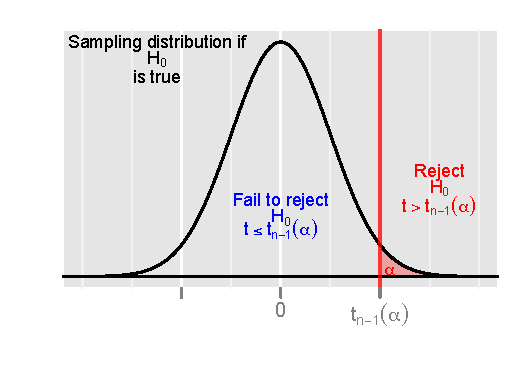
\includegraphics[width=0.5\textwidth]{diagram.pdf}}
\caption{Decision regions  for classical inference for $H_0: \mu=\mu_0$ vs $H_a:\mu>\mu_0$.}
\label{classical}
\end{figure}

Type I error, is the probability of rejecting the null hypothesis $H_0$ when $H_0$ is true. Type II error, denoted by $\beta$ is the probability of failing to reject the null hypothesis $H_0$ when $H_0$ is false. Type I error is committed in a jury trial when it is decided that a not guilty person is  ``guilty''. This is a serious mistake as an innocent person is punished. Type II error is committed when there is a guilty person is not convicted, not considered to be so serious. The power of a statistical test is defined as the probability that the test will reject $H_0$ when $H_0$ is false i.e the power of the test is the probability of correctly rejecting a false null hypothesis. So the power is the probability of not committing a Type II error and hence is denoted by 1 - $\beta$. (\cite{casella:2002} and \cite{lehman:1997} give more thorough treatments of hypothesis testing.)
 
%More generally, let $\theta$ be a population parameter of interest, with $\theta$ $\in$ $\Theta$, the parameter space. Any null hypothesis $H_0$ then partitions the parameter space into $\Theta_0$ and $\Theta_0^c$ with $H_0: \theta \in \Theta_0$ versus $H_a: \theta  \in \Theta_0^c$ as defined in \cite{casella:2002}. \\

%Let $\chi$ be the set of all possible values of $\mathbf{X} = (X_1, \dots, X_n)$. Then a test function or a test rule $\phi(X_1, \dots, X_n)$ is a function from $\chi$ into [0, 1] with the interpretation that if $\mathbf{X} = (X_1, \dots, X_n)$ is observed then $H_0$ is rejected with probability $\phi( \mathbf{X})$. Hence the following definitions:
%\begin{itemize}
%\item Probability of Type I error at $\theta \in \Theta_0$ is $E_{\theta} \phi(\mathbf{X})$. 
%\item Probability of Type II error at $\theta \in \Theta_0^c$ is $1 - E_{\theta} \phi(\mathbf{X})$. \item Size or the level of the test function $\phi(\mathbf{X})$ is given by $\max_{\theta \in \Theta_0} E_{\theta} \phi(\mathbf{X}) $.
%\item Power function of $ \phi(\mathbf{X})$ is given by $\Pi_{\phi}(\theta) = E_{\theta} \phi(\mathbf{X})$.
%\end{itemize}


\section{Introduction to Visual Inference} 

\citet{buja:2009} proposes visual statistical methods with an inferential framework. In visual inference the plots take on the role of test statistics, the test statistic is a visual representation of the data, not a numerical value. Comparison data is generated under the assumption that the null hypothesis is true, and plots of this data are generated. These plots, known as the null plots gives the ``null distribution of plots'' analogous to the null distribution of test statistics. The plot of the data is compared with the null plots. Variations of these ideas have historically been utilized for data analysis, albeit sparingly, which is commented in the introduction of \cite{buja:2009}. \cite{gelman:2004} puts these ideas in the context of model building. The key feature of \cite{buja:2009} is that it makes the connection to the process of hypothesis testing, and quantifying significance. There are two protocols defined in this paper.

\subsection{Protocols of Visual Inference} \label{sec:protocol} \citet{buja:2009} introduces two protocols for graphical inference: one is the  ``Rorschach'' and the other is the ``lineup''. The purpose of the Rorschach protocol is to measure a data analyst's tendency to over interpret plots in which there is no or spurious structure. On the other hand the lineup provides a simple inferential process to produce a valid p-value for the observed plot. Here we describe the protocols briefly and refer the reader to \citet{buja:2009} and \cite{hadley:2010} for more details. 

\begin{itemize}
\item {\bf Rorschach:} It is possible that the randomness of the data inherits some pattern in the plot. The Rorschach protocol is designed to expose the data analyst's tendency of over-interpretation of patterns when there is actually no or spurious structure. The results are specific to a particular data analyst and a particular data analysis procedure. The protocol estimates the effective family-wise Type I error rate. A data administrator may generate the null plots and decides about the prior information that the data analyst is provided. The administrator may program the series of null plots in such a way that the plot of the real data is inserted in a random location. A toned-down version may also be used for self training. This self training may improve the family-wise error rate of the data analyst and develop an awareness of the features they are most likely to spuriously detect. 
%The human eye can see pattern while there is no pattern in deed. This protocol helps understand the extent of this pattern in the null plots. The process includes asking readers to report what they see in null plots. This helps reader getting acquainted with the natural patterns due to completely randomness. 
The Rorschach protocol is named after the (pop-)psychology Rorschach test, in which subjects interpret abstract ink blots. 

\item {\bf Lineup:} The lineup protocol gets its name after the police lineup of criminal investigation. In a police lineup, the accused is placed among a set of innocent people who may be prisoners, actors or volunteers having no connection with the case. The witness is asked to pick from this lineup. Likewise in a lineup protocol, the accused which is the observed plot is placed randomly among a set of null plots, say $m$, and the witness (in this case the viewer) is asked to identify the plot as most different from the others. If the viewer  can correctly identify the observed plot from the lineup, we have reasons to believe that the observed plot has a specific pattern which is missing in the null plots. This protocol leads to the development of the technique of visual inference by defining the test statistic as a plot that mostly show a specific pattern in the data when alternative hypothesis is true. Figure \ref{lineup} shows a typical lineup. 
\end{itemize}

Let us consider the following example. The data represents the concentration of a metal in mg/kg for two sites A and B.
%Model : $Y_i$ = $\beta_0$ + $\beta_1 X_i$ + $\epsilon_i$, \qquad $\epsilon_i \stackrel{iid}{\sim} N(0, \sigma^2)$ \\
%\vspace{0.1cm}
We want to test whether there exists a significant difference between the concentration levels in the two sites A and B. Let $\mu_1$ denote the mean concentration level in Site A and $\mu_2$ denote the mean concentration level in Site B. To test that, we have the following null and alternative hypothesis:
\[
H_0: \mu_1 = \mu_2 \qquad \hbox{versus} \qquad H_a: \mu_1 \ne \mu_2
\]
%\vspace{0.4cm}
(Technically the problem this data addressed was more interested in testing a one-sided alternative, whether site B has higher concentration than site A, but it is more interesting for this example to consider the two-sided alternative hypothesis.) The test statistic is the plot of the real data. The 19 null plots are generated by assuming that null hypothesis $H_0: \mu_1 =  \mu_2$ is true. So we permute the class variable site to obtain the null plots keeping the other variables fixed. The observed plot is placed randomly among these 19 plots in a lineup given in Figure \ref{lineup}. The viewer is asked to identify the plot which is most different. If the viewer can identify the plot of the real data, we will have reasons to believe that the observed plot has a pattern which is absent in the null plots. So we would reject the null hypothesis. If the viewer cannot identify the observed plot, we fail to reject the null hypothesis. 
%\newpage

\begin{figure}[hbtp]
%\begin{figurehere}
   \centering
       \scalebox{1}{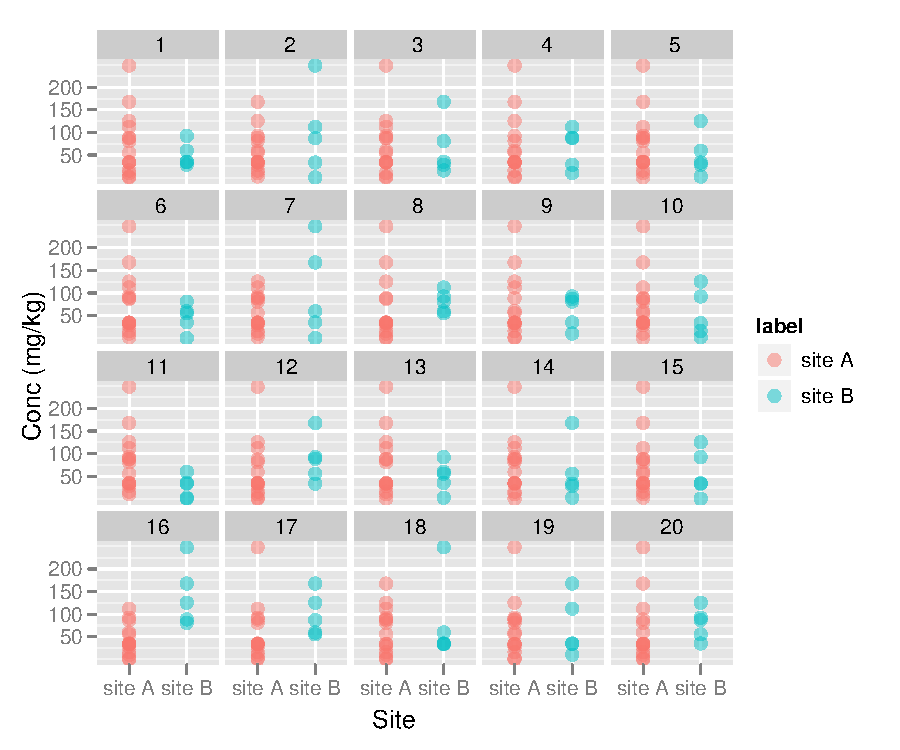
\includegraphics{lineup-dot.pdf}}
      \caption{A typical lineup plot ($m = 20$) for testing $H_0: \mu_1 =  \mu_2$. 
      % \qquad vs \qquad H_a: \beta_1 \ne 0$
      When the alternative hypothesis is true the observed plot should have the largest vertical difference between the centers. Can you identify the observed plot?}
      \label{lineup}
%	\vspace{-.1in}
\end{figure}

%\newpage

Plot 16 is the plot of the real data. If the viewer could identify the plot then we have reasons to believe that there exists a statistically significant difference between the mean concentration levels in site A and site B. So the lineup protocol is the basis of the visual inference while the Rorschach protocol helps viewer understand the extent of randomness. 

\cite{majumder:2013} describes a comparative study between the visual inference method and the classical inference methods, focusing on plots that might be used in linear modeling. In his work the expected power of the visual test is compared with the power of the uniformly most powerful (UMP) test. The power of the visual test is computed by responses from several large samples of lineup evaluators recruited through Amazon Turk \citep{turk}. The results suggest that the expected power of a visual test is almost as good as the power of UMP test, that visual inference compares favorably with classical testing, in the traditional setting where the classical test performs well. They established properties and efficacy of visual testing procedures in order to use them in situations where traditional test cannot be used. In addition \cite{majumder:2013} provide a nice way of making the leap traditional hypothesis testing to visual inference. We have adapted that table for the $H_0: \mu_1 =  \mu_2$ vs $H_a: \mu_1 \ne \mu_2$ example described and plotted in Figure \ref{lineup}, which can be seen in Table \ref{tbl:compare}.

%\newpage

\begin{table*}[hbtp]
\caption{Comparison of visual inference with traditional hypothesis testing.}
\centering 
\begin{tabular}{llll} 
\hline
  & Mathematical Inference &  Visual Inference \\ %[0.5ex] % inserts table %heading 
\hline
  Hypothesis & $H_0: \mu_1= \mu_2$ vs $H_a: \mu_1 \ne \mu_2$& $H_0: \mu_1 = \mu_2$ vs $H_a: \mu_1 \ne \mu_2$\\
%  \vspace{0.5cm}	
 & \begin{minipage}[h]{1.5cm} \begin{center} \scalebox{0.35}{
\includegraphics{down_arrow.pdf}} \end{center} \end{minipage} & \begin{minipage}[h]{1.5cm} \begin{center} \scalebox{0.35}{
\includegraphics{down_arrow.pdf}} \end{center} \end{minipage} \\
%\vspace{0.5cm}				  
 Test Statistic & $T(y)=\frac{\bar{y}_1 - \bar{y}_2}{s\sqrt{\frac{1}{n_1} + \frac{1}{n_2}}}$ & $T(y)=$ \begin{minipage}[h]{1cm} \begin{center} \scalebox{0.35}{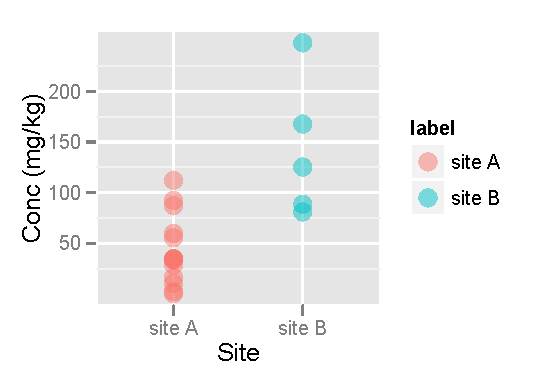
\includegraphics{data-dot.pdf}} \end{center} \end{minipage} \\
				 
 & \begin{minipage}[h]{1.5cm} \begin{center} \scalebox{0.35}{
\includegraphics{down_arrow.pdf}} \end{center} \end{minipage} & \begin{minipage}[h]{1.5cm} \begin{center} \scalebox{0.35}{
\includegraphics{down_arrow.pdf}} \end{center} \end{minipage} \\
				 
 Sampling Distribution & $f_{T(y)}(t); $\begin{minipage}[h]{1.5cm} \begin{center} \scalebox{0.5}{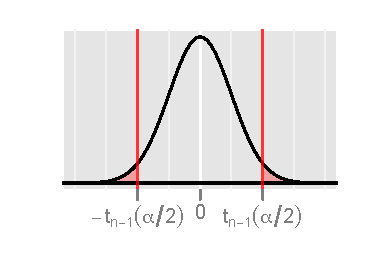
\includegraphics{two-sided-rejection.pdf}} \end{center} \end{minipage} & $f_{T(y)}(t); $ \begin{minipage}[h]{1.5cm} \begin{center} \scalebox{0.29}{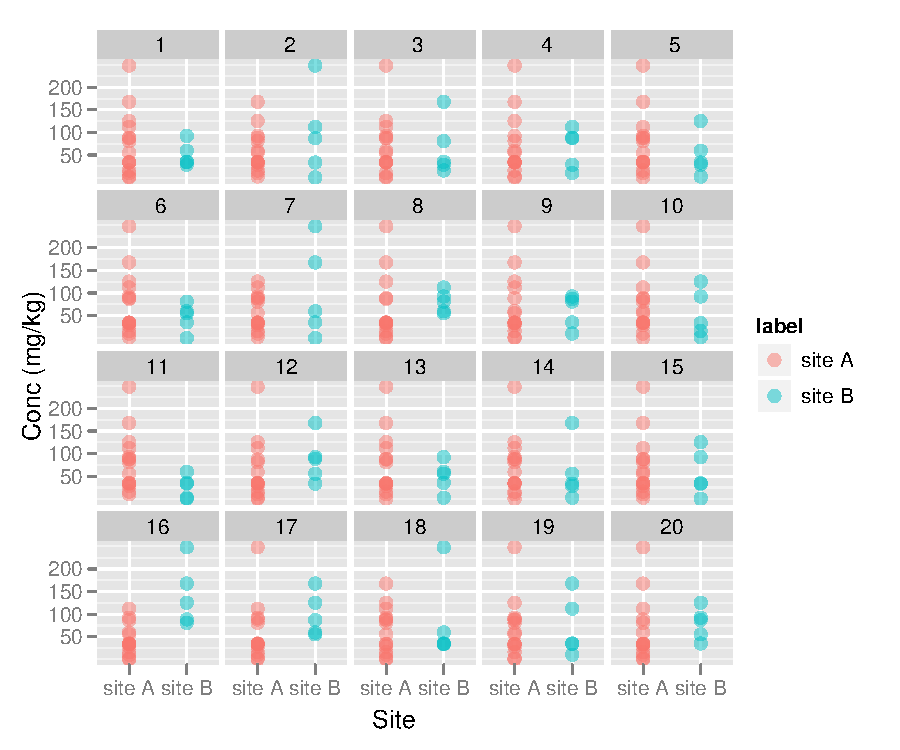
\includegraphics{lineup-dot.pdf}} \end{center} \end{minipage} \\
 & \begin{minipage}[h]{1.5cm} \begin{center} \scalebox{0.35}{
\includegraphics{down_arrow.pdf}} \end{center} \end{minipage} & \begin{minipage}[h]{1.5cm} \begin{center} \scalebox{0.35}{
\includegraphics{down_arrow.pdf}} \end{center} \end{minipage} \\
 Reject $H_0$ if & observed $T$ is extreme & observed plot is identifiable \\
\hline 
\end{tabular}
\label{tbl:compare}
\end{table*}	

\begin{figure}[hbtp]
%\begin{figurehere}
   \centering
       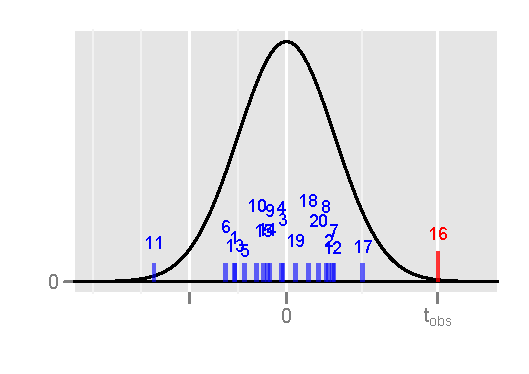
\includegraphics[width=0.5\textwidth]{visual-inference-plot-1.pdf}
      \caption{Sampling distribution of the test statistic with the observed value and the values for the null plots corresponding to the lineup in Figure \ref{lineup}.}
      \label{visual-plot}
%	\vspace{-.1in}
\end{figure}

In traditional hypothesis testing the sampling distribution of the test statistics is continuous, which allows evaluation of probability on an infinite spectrum. With the lineup, although conceptually we may have an infinite collection of plots from the null distribution, in practice, we sample a finite number of null datasets to generate the lineup. A human judge has a physical limit on the number of null plots they can peruse. This poses one of the issues with using the lineup protocol.  Figure \ref{visual-plot} gives the sampling distribution (black curve) for the $t$-distribution, along with the $t$-statistics of the samples that were drawn from the null distribution (blue bars) and that of the observed data (red bar) for the plots in the lineup shown in Figure \ref{lineup}. Effectively,  in visual inference the red line is compared only to these finite number of blue lines visually to make a decision, unlike classical inference where we look at the rejection region (Figure \ref{classical}) to make decisions. So as Tukey suggested, there may be a ``bad'' random sample of null plots which may affect our decision. This is a major component of this thesis research to we develop techniques to determine the quality of a lineup. In practice, though, it needs to be noted, that visual inference will not typically be used in applications where there is an existing classical test. The purpose of visual inference is not to compete with classical statistics -- its purpose is to provide formalism and quantification in problems where there are none, currently. For the purposes of research and assessment we use the classical setting because it provides benchmarks for how visual inference will likely perform.

%\begin{figure}[hbtp]
%%\begin{figurehere}
%   \centering
%       \scalebox{0.5}{\includegraphics{visual-inference-plot.pdf}}
%      \caption{Null Distribution of the test statistic with the observed value and the values for the null plots.}
%      \label{visual-plot-0}
%%	\vspace{-.1in}
%\end{figure}
 


%\begin{table*}[hbtp]
%\caption{Comparison of visual inference with existing inference technique}
%\centering 
%\begin{tabular}{llll} 
%\hline
%  & Mathematical Inference &  Visual Inference \\ %[0.5ex] % inserts table %heading 
%\hline
%  Hypothesis & $H_0: \beta=0$ vs $H_a: \beta \ne 0$& $H_0: \beta=0$ vs $H_a: \beta \ne 0$\\
%%  \vspace{0.5cm}	
% & \begin{minipage}[h]{1.5cm} \begin{center} \scalebox{0.25}{
\includegraphics{down_arrow.pdf}} \end{center} \end{minipage} & \begin{minipage}[h]{1.5cm} \begin{center} \scalebox{0.25}{
\includegraphics{down_arrow.pdf}} \end{center} \end{minipage} \\
%%\vspace{0.5cm}				  
% Test statistic & $T(y)=\frac{\hat{\beta}}{se(\hat{\beta})}$ & $T(y)=$ \begin{minipage}[h]{1cm} \begin{center} \scalebox{0.12}{\includegraphics{test-plot.pdf}} \end{center} \end{minipage} \\
%				 
% & \begin{minipage}[h]{1.5cm} \begin{center} \scalebox{0.25}{
\includegraphics{down_arrow.pdf}} \end{center} \end{minipage} & \begin{minipage}[h]{1.5cm} \begin{center} \scalebox{0.25}{
\includegraphics{down_arrow.pdf}} \end{center} \end{minipage} \\
%				 
% Null Distribution & $f_{T(y)}(t); $\begin{minipage}[h]{1.5cm} \begin{center} \scalebox{0.12}{\includegraphics{stat_mathematical_test.pdf}} \end{center} \end{minipage} & $f_{T(y)}(t); $ \begin{minipage}[h]{1.5cm} \begin{center} \scalebox{0.19}{\includegraphics{stat-lineup.pdf}} \end{center} \end{minipage} \\
% & \begin{minipage}[h]{1.5cm} \begin{center} \scalebox{0.25}{
\includegraphics{down_arrow.pdf}} \end{center} \end{minipage} & \begin{minipage}[h]{1.5cm} \begin{center} \scalebox{0.25}{
\includegraphics{down_arrow.pdf}} \end{center} \end{minipage} \\
% Reject $H_0$ if & observed $T$ is extreme & observed plot is identifiable \\
%\hline 
%\end{tabular}
%\label{tbl:compare}
%\end{table*}	


%In their paper \citet{buja:2009} presented some of the issues related to visual inference. For example the wording of the instruction for viewers while evaluating lineup plots, information related to the viewers responses, effect of colors or gaps in the plot on the responses. These issues need to be examined before more general implementation of visual inference. In my thesis work I intend to address these issues elaborately.

%\subsection{Evaluation of the Lineup Plots} Single or multiple observer can evaluate a lineup plot. If a individual observer evaluates a lineup of $m$ plots, the p-value is reported as $\le \frac1m$ when the null hypothesis is rejected and $\ge 1-\frac1m$ when the null hypothesis could not be rejected. For for a pool of $K$ observers we have $$ U \sim Binom(K,\frac1m)$$ where $U$ is the number of successful evaluations. Thus we have the p-value as $$Pr(U \ge u)= \sum_{k \ge u}^K {{K \choose k} (\frac1m)^k(1-\frac1m)^{(K-k)}}$$ where $u$ be the observed number of successful evaluations. Due to the discrete nature of binomial distribution this p-value is conservative.
%
%The type-I error probability is fixed to be $\frac1m$ as per the design of the lineup plot.

\section{Overview}

My research extends the visual inference methodology in two ways -- by producing metrics to quantify lineups and examine how people read statistical plots, and examining how it applies to assessing dimension reduction in high dimension low sample size (HDLSS) problems. 

Chapter \ref{ch:largepsmalln} explores the performance of dimension reduction methods such as  projection pursuit for high dimension, low sample size (HDLSS) data. The key points of interest were producing a way to evaluate an algorithm when its results are primarily visual, and to examine how well people can distinguish between real separation and noise in HDLSS data.  Several human subjects experiment were conducted using simulated data to provide controlled conditions. Results suggest that people can detect real separation from pure noise up to a reasonably high dimension. The broader community still has difficulty in understanding HDLSS data, which can be seen by published papers where the authors get excited about structure in low-dimensional projections, when it is really present simply because of the sparseness of high-dimensions. This chapter suggests that the lineup protocol can potentially explain HDLSS issues effectively. This paper is accepted for publication by Computational Statistics. \\

Chapter \ref{ch:metrics} focusses on developing metrics to describe the quality of a lineup. In conventional inference, the test statistic is compared to all possible values of the sampling distribution, but in visual inference only a finite number of plots are drawn randomly from the sampling distribution. Understanding the effect of these finite comparisons is important. This chapter develops a variety of distance metrics that can be used to measure the ``closeness'' of observed data plot with the null plots. These metrics are compared to the results from human subjects experiments. These metrics may be useful to learn how people detect the observed data plot from the null plots. For example, with the HDLSS simulations, traditional class separation metrics like WBratio do not match the results from people as well as a metric measuring the gap between clusters. \\

Chapter \ref{ch:nullabor} describes the R package \textbf{nullabor} which generates the lineup plots automatically if the observed data and the null generating mechanism are provided. Routines to calculate the distance metrics on the lineup were added. Some common distance metrics are included in the package and users have the freedom of using their own distance metrics. The package also provides diagnostic plots for comparing a lineup with other possible lineups that may have been generated. \\

%Chapter \ref{ch:teaching} develops teaching materials to improve statistical thinking among undergraduate students and among people who are familiar with statistical methods. \\ 
%
%Chapter \ref{ch:application} would most likely use the lineup protocol to make inference in a large $n$ setting. The goal is to examine how the visual inference procedure works in a real life situation. This chapter also looks at the ``sufficient'' statistic. \\

Finally, chapter \ref{ch:conclusion} provides a summary of the dissertation and discussion of possible future research work. 

\section{Scope of my Research}

This dissertation provides the ground work for the application of visual inference. It applies visual inference methods in a high dimension, low sample size (HDLSS) framework, including using it to show that a gene expression data set does not have the separate clusters as claimed. The research has initiated ideas on metrics that could be used to evaluate the effect of the finite set of null plots in a lineup, cross-validate observer data, and help understand observer responses.  Finally, an open source package has been extended to include this new metric methods to improve the use of the lineup protocol for visual inference. 


%\section{Validation of the Protocols}
%
%\citet{buja:2009} suggested evaluating the performance of the protocols using \cite{turk} Mechanical Turk web site. The goal is to estimate the family-wise Type I error rates for each data situation. This web site also allows us to keep record of time taken to complete a task, the reason why the individuals pick in a lineup, together with a confidence rating. Turk worker do not necessarily make-up of a representative population sample. Thus to make a correction of this selection bias we can collect some demographic information such as age, gender, education level or location of the worker. The Mechanical Turk has also been used to collect data for the Fleshmap project by \cite{viegas:2008}.
%
%We have done couple of turk studies and some results are displayed in chapter \ref{ch:regression}. More results are to be presented in chapter \ref{ch:turk} and \ref{ch:turk_analysis}.
%
%\section{Background}Statistical graph or plot of data has its presence way before the development of the classical inference procedures. The first recorded instance of statistical graphics based on the data was known to be in the year 1644 (variations in determination of longitude between Toledo and Rome as illustrated by \cite{friendly:2001}). The development of fundamental classical inferential procedures took around two hundred years from Bernoulli through Fisher (1713 to 1935 as per \cite{hald:2004}). 
%
%I intend to write down a little history of the statistical graphics in this section. The goal is to identify why the graphics were not used as a tool for statistical inference even though we see its presence way before the development of classical inference techniques. One factor could be the absence of modern computing facilities. But to what extent does the lack of computing facility prevent statistical graphics from being used as the tool for statistical inference?
%
%
%\section{Explanation of chapters and scope} I described some materials that I intend to include in chapter \ref{ch:introduction}. While one of our goals is to analyze the performance of the lineup protocol in finding the pattern of the data when it is actually present we have specific focuses in the different chapters. These are described below;
%
%Chapter \ref{ch:regression} develops the visual inference procedure for a simple linear regression setting with normally distributed error structure. The purpose is to show how the visual inference technique perform in the very fundamental inferential procedure. This chapter also provides the various methods of obtaining power of the proposed visual test. The results obtained from the human subject experiment is stunning and the paper based on these findings won the ASA student paper competition 2011. 
%
%Chapter \ref{ch:turk} describes the procedure of designing an Amazon Mechanical Turk experiment to evaluate the performance of visual inference technique. This explains the detailed factors to be considered while running the experiment. 
%
%Chapter \ref{ch:turk_analysis} is designed to present analysis of the data obtained from various turk experiments. The focus is to identify whether demographical factors are influential in visual evaluation of plots. The time taken for each evaluation may depend on the difficulty level of the plot. This will allow us to come up with some measure for the difficulty level of each lineup plot. 
%
%Chapter \ref{ch:application} focuses on the real data study. The goal is to examine how the visual inferential procedure perform in the case of real data. We intend to study the performance of line up protocols with the real data and compare them with what we obtained from simulated data.
%
%Finally chapter \ref{ch:conclusion} displays my completed tasks so far as well as the plans and timelines of my work for the next year. Some of the future directions of research are also described even though they may not be under the scope of this dissertation work. 
 

%\pagenumbering{arabic}
%% ================ chapter 2 starts here  ==========================

\chapter{USING VISUAL STATISTICAL INFERENCE TO BETTER UNDERSTAND RANDOM CLASS SEPARATIONS IN HIGH DIMENSION, LOW SAMPLE SIZE DATA}\label{ch:largepsmalln}
\vspace{0.8cm}
%Niladri Roy Chowdhury, 
%Dianne Cook,
%Heike Hofmann, 
%Mahbubul Majumder,\\
%Eun-Kyung Lee,
%Amy L. Toth\\
\begin{center}
\large{A paper accepted by \it{Computational Statistics}.}

\large{Niladri Roy Chowdhury, Dianne Cook, Heike Hofmann, Mahbubul Majumder}\\
\large{Eun-Kyung Lee, Amy L. Toth}
\end{center}

%
%\institute{Niladri Roy Chowdhury, Dianne Cook, Heike Hofmann, Mahbubul Majumder \at
%              Department of Statistics, Iowa State University, Ames, IA, USA \\
%              \email{niladrir@iastate.edu, dicook@iastate.edu, hofmann@iastate.edu, mahbub@iastate.edu}        
%           \and
%           Eun-Kyung Lee \at
%           Department of Statistics, EWHA Womans University, Seoul, Korea\\
%           \email{lee.eunk@gmail.com}
%           \and 
%           Amy L. Toth \at
%           Departments of Ecology, Evolution, and Organismal Biology and Entomology, Iowa State University, Ames, IA, USA \\
%           \email{amytoth@iastate.edu}
%}
%
%\date{Received: date / Accepted: date}

%\maketitle

\section*{Abstract}
Statistical graphics play an important role in exploratory data analysis, model checking and diagnosis. With high dimensional data, this often means plotting low-dimensional projections, for example, in classification tasks projection pursuit is used to find low-dimensional projections that reveal differences between labelled groups. In many contemporary data sets the number of observations is relatively small compared to the number of variables, which is known as a high dimension low sample size (HDLSS) problem. This paper explores the use of visual inference on understanding low-dimensional pictures of HDLSS data. Visual inference helps to quantify the significance of findings made from graphics.  This approach may be helpful to broaden the understanding of issues related to HDLSS data in the data analysis community. Methods are illustrated using data from a published paper, which erroneously found real separation in microarray data, and with a simulation study conducted using Amazon's Mechanical Turk.

\textbf{keywords} : statistical graphics , lineup, visualization , projection pursuit, data mining





\section{Introduction} 

Many problems needing solutions today require the analysis of data where more variables are measured than there are samples taken. This is commonly referred to as high dimensional, low sample size (HDLSS) data (see for e.g. \cite{hall:2005}).   
HDLSS data occur in many application areas like face recognition, spectroscopy  and gene expression analysis. Classical statistical methods often fail in this context, because of insufficient data to support for parameter estimation. 

Reducing the dimension, using principal component analysis (PCA), would be a classical first step in the analysis of HDLSS data. PCA requires estimating the eigenvalues (maximum variance) and eigenvectors (direction of maximum variance) of the population variance-covariance based on the sample. With insufficient data this is a Sisyphean task. Just imagine, estimating a line on the foundation of a single point - there are infinitely many possibilities for lines. For classification tasks, finding a low-dimensional space where the classes are separated is a common first step. Linear discriminant analysis (LDA) is the classical approach. LDA solves an eigenvalue decomposition problem comparing distances between group means with variance around each mean. Estimating the variance-covariance is problematic when there are few points. In addition, when there are few sample points in high dimensions, differences between groups can be found in many different low-dimensional spaces, simply because of the sparseness of space.

\cite{marron:2007} describes the estimation issues associated with HDLSS.  
%One of the problems with HDLSS data is that not all the measured variables are ``important'' for understanding the underlying phenomenon of interest. 
Advancements in PCA to handle HDLSS data have been done by \cite{marron:2011} and \cite{yata:2010}. \cite{donoho:2009} and \cite{donoho:2008} study optimal variable selection and introduce a principle of model selection for problems where only a small fraction of the variables are useful and unknown. Penalization is another common approach to handle HDLSS, and has been applied to classification problems e.g. \citep{witten:2011, lee:2009}. Estimates of the variance-covariance are obtained by an interpolation with the identity matrix, effectively reducing the importance of some variables. 

So, although substantial research has produced many new approaches to creating better models and estimation for HDLSS data, the major issues are still not clear to many data analysts. For example, \cite{toth:2010} make a common mistake of seeing structure where none exists. Figure \ref{oligo} reproduces the result in this paper.  They use LDA to examine gene expression data of wasps containing 447 variables and 50 cases. There are 50 different paper wasps divided into 4 types: Foundress (F), Gyne (G), Queen (Q) and Worker (W), 14  wasps of type Foundress and 12 each of the other 3 types. The authors, knowing that LDA requires that the dimension ($p$) should be smaller than the number of observations ($n$), first reduced the dimension from 447 to 40 by randomly selecting a subset of significantly different oligonucleotides. LDA produced a 2D projection ($d=2$) of best separation. This is almost the same approach as used in \cite{dudoit:2002}, one of the first studies of classification of gene expression data. What results is a picture of the four groups that suggests big differences in the types of wasps. There exists no conventional inferential method that enables us to conclude whether this apparently clear separation is statistically significant or not. For prediction, typically data is broken into training and test sets, or cross-validation is conducted to assess the significance of difference, using test set error. This approach does not work well for visualization.

\begin{figure*}[hbtp]
   \centering
       \scalebox{.45}{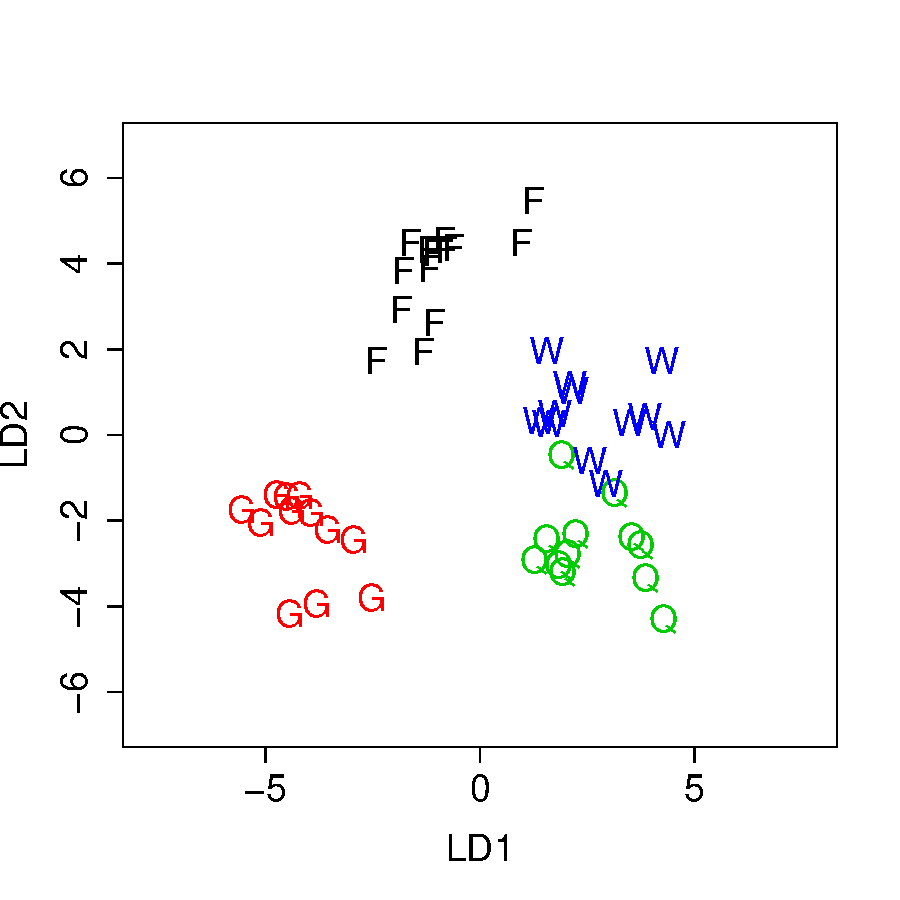
\includegraphics{Images/toth_lda.pdf}}
       \caption{LD1 versus LD2 from an LDA on a randomly selected subset of 40 significantly different oligos : F, Foundress; G, gyne; Q, queen and W, worker. It can be noticed that the groups F and G are separated. This plot is generated to match Figure 2 in \cite{toth:2010}. }
     \label{oligo}
\end{figure*}  

We propose that new methods for inference on graphics might be helpful for building understanding very generally. Visual statistical inference was first conceptually introduced by \cite{buja:2009}, formalized and validated by \cite{majumder:2013}. Using visual inference, it can be shown that there is no real difference between the wasp groups - what you see is a mirage. 

Visual inference may also be useful in related applications, such as checking algorithms that produce visual results. We used the approach described in this paper to check the optimization algorithm of projection pursuit in the \texttt{tourr} package \citep{tourr:2011} in \texttt{R} \citep{r}. The optimization procedure was new, and we suspected that it was being sensitive to the order of data values, and returning projections of purely noise data that we thought were surprisingly distinct from noise. Visual inference was able to temper our concerns.   

This paper describes visual statistical inference as applied to dimension reduction for HDLSS. In particular we focus on dimension reduction using projection pursuit, and the effect that having high dimension has on the robustness of the separation between groups.  Small simulation experiments are used to examine the problem in a controlled setting. The next section explains visual inference methods. Section \ref{sec:dimred} discusses the dimension reduction methods. Section \ref{sec:turk} describes Amazon's Mechanical Turk  \citep{turk}  which was used to conduct the experiment. The application of visual inference methods on the wasp data (\cite{toth:2010}) is described in Section \ref{sec:wasp}. Section \ref{sec:experiment} discusses the experiment designed to examine people's perception of separation in the presence of real separation and ``purely noise'' for simulated HDLSS data. Section \ref{sec:results} discusses the collected data and results. 


\section{Visual inference methods} \label{sec:inference}

\cite{buja:2009} proposed two protocols, the Rorschach and the lineup. While the Rorschach protocol helps to understand the extent of randomness, the lineup protocol is  used for testing significance of findings. These methods together are called visual statistical inference. \cite{majumder:2013} made a head-to-head comparison between visual statistical inference tests and classical tests which showed that the lineup protocol performs similarly to the classical tests. Unlike classical hypothesis testing, the test statistic in visual inference is not numeric, but a plot that is appropriately chosen to display a  distinctive pattern in case that the null hypothesis is false. The lineup protocol of size $m$ embeds the observed data plot amongst ($m$ - 1) null plots. Null plots are created by a mechanism consistent with the null hypothesis. Human subjects are asked to identify the plot in the lineup with the most distinct feature(s). When the alternative hypothesis is true, it is expected that the plot of the observed data, the test statistic, will have visible feature(s) inconsistent with the null hypothesis. If the subjects choose the plot of the observed data, this is evidence against the null hypothesis and with enough support, the null hypothesis is rejected. 

An illustration of the lineup protocol in contrast to the conventional test is shown in Table \ref{tbl:compare}. Both start with the same hypothesis but the test statistic in a conventional setting is the parameter estimate divided by its standard error. In visual inference the test statistic is a plot of the observed data. In this case, a dot plot is used since the variable of interest is continuous with two groups. In a conventional test the value of the test statistic is compared with all possible values of the sampling distribution, the distribution of the test statistic if the null hypothesis is true. If it is extreme, then the null hypothesis is rejected. In visual inference, the plot of the data is compared with a finite number of samples drawn from the sampling distribution. If the actual data plot is selected as the most different, then the null hypothesis is rejected. 

\begin{table*}[hbtp]
\centering 
\caption{Comparison of visual inference with traditional hypothesis testing. Starting with the same hypothesis, the test statistic in a conventional setting is a real number while in visual inference it is a plot of the observed data. In conventional testing the value of the test statistic is compared with all possible values of the sampling distribution. $H_o$ is rejected if it is extreme. In visual inference, the plot of the data is compared with a finite number of samples drawn from the null distribution. If the actual data plot is identifiable, then the null hypothesis is rejected. 
}
\begin{tabular}{llll} 
\hline
  & Mathematical Inference &  Visual Inference \\ 
\hline
  Hypothesis & $H_o: \mu_1= \mu_2$ vs $H_a: \mu_1 \ne \mu_2$& $H_o: \mu_1 = \mu_2$ vs $H_a: \mu_1 \ne \mu_2$\\
%  \vspace{0.5cm}	
 & \begin{minipage}[h]{1.5cm} \begin{center} \scalebox{0.25}{
\includegraphics{down_arrow.pdf}} \end{center} \end{minipage} & \begin{minipage}[h]{1.5cm} \begin{center} \scalebox{0.25}{
\includegraphics{down_arrow.pdf}} \end{center} \end{minipage} \\
%\vspace{0.5cm}				  
 Test Statistic & $T(y)=\frac{\overline{y}_1 - \overline{y}_2}{s\sqrt{\frac{1}{n_1} + \frac{1}{n_2}}}$ & $V(y)=$ \begin{minipage}[h]{1cm} \begin{center} \scalebox{0.35}{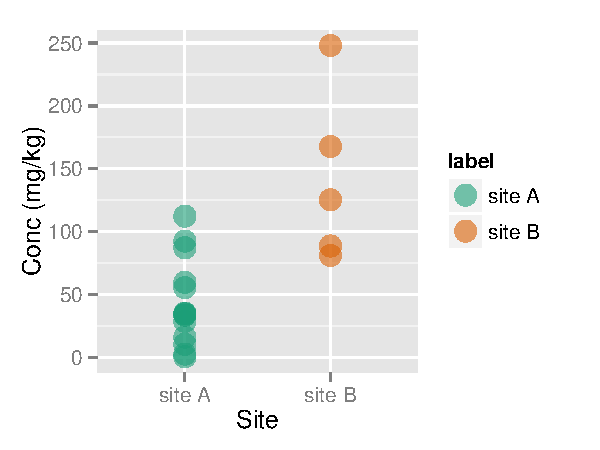
\includegraphics{data-dot-rev.pdf}} \end{center} \end{minipage} \\
				 
 & \begin{minipage}[h]{1.5cm} \begin{center} \scalebox{0.25}{
\includegraphics{down_arrow.pdf}} \end{center} \end{minipage} & \begin{minipage}[h]{1.5cm} \begin{center} \scalebox{0.25}{
\includegraphics{down_arrow.pdf}} \end{center} \end{minipage} \\
				 
 Sampling Distribution & $f_{T(y)}(t); $\begin{minipage}[h]{1.5cm} \begin{center} \scalebox{0.5}{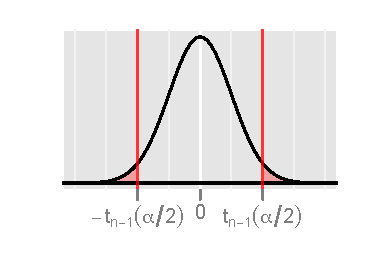
\includegraphics{two-sided-rejection.pdf}} \end{center} \end{minipage} & $f_{V(y)}(t); $ \begin{minipage}[h]{1.5cm} \begin{center} \scalebox{0.29}{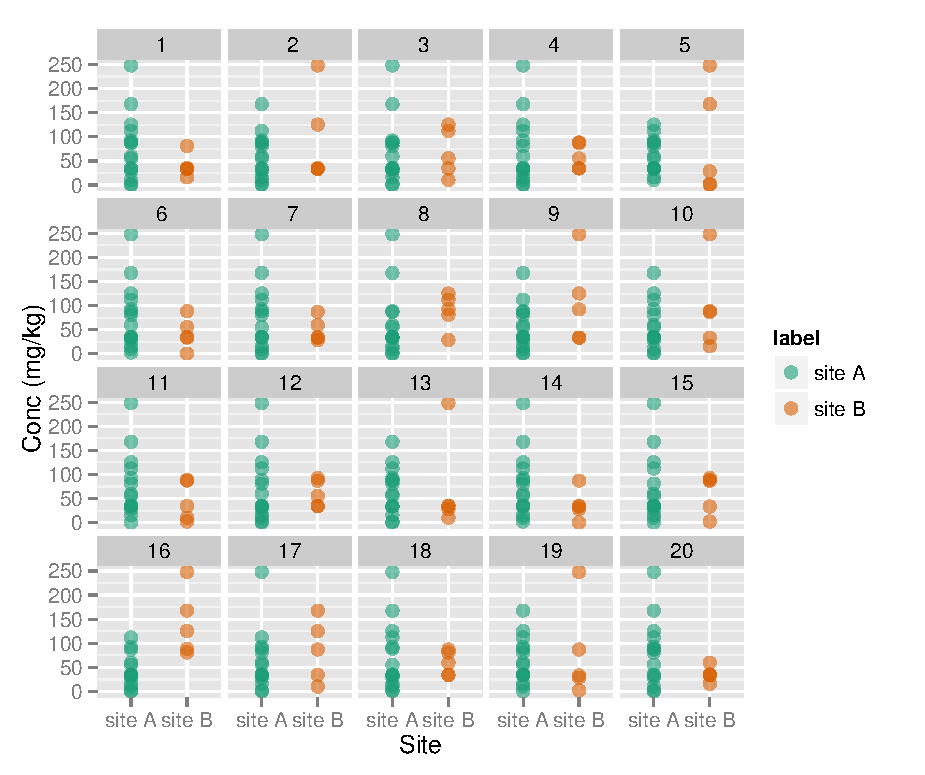
\includegraphics{lineup-dot-rev.pdf}} \end{center} \end{minipage} \\
 & \begin{minipage}[h]{1.5cm} \begin{center} \scalebox{0.25}{
\includegraphics{down_arrow.pdf}} \end{center} \end{minipage} & \begin{minipage}[h]{1.5cm} \begin{center} \scalebox{0.25}{
\includegraphics{down_arrow.pdf}} \end{center} \end{minipage} \\
 Reject $H_o$ if & observed $T$ is extreme & observed data plot is identifiable \\
\hline 
\end{tabular}
\label{tbl:compare}
\end{table*}


For example, suppose we have two sample data on the concentration of a metal in $mg/kg$ for sites A and B of sizes $n_1$ and $n_2$ respectively. We want to test whether there exists a difference between the concentration levels in the two sites A and B. To test for statistically significant difference between the two populations from which the data was sampled, let $\mu_1$ denote the mean concentration level in Site A and $\mu_2$ denote the mean concentration level in Site B. Thus the null and alternative hypothesis would be
\[
H_o: \mu_1 = \mu_2 \qquad \hbox{versus} \qquad H_a: \mu_1 \ne \mu_2
\]
The conventional test would be a two-sample t-test with test statistic $T(y)$ described in Table \ref{tbl:compare}. One way to plot this data is a side-by-side dotplot. Let this be the visual test statistic $V(y)$. Null plots are generated assuming that $H_o$ is true. Here, this is achieved by randomly permuting the site label. The observed data plot is placed randomly among the null plots to obtain a lineup. In this example, $m = 20$ is the size of the lineup - there are 19 null plots. If $H_o$ is not true, the dots of one group should be vertically shifted relative to the other group. If the human observer can identify the plot of the real data, there will be reason to believe that the observed data plot has a pattern which is absent in the null plots leading to a rejection of the null hypothesis. If the viewer cannot identify the observed data plot, we fail to reject the null hypothesis. Under the null hypothesis, each observer has a $1/m$ chance of picking the observed plot from a lineup of size $m$. Hence $1/m$ is the minimal value at which we can set the Type I error, $\alpha$, consistent with $\alpha = 0.05$ if $m = 20$.  \cite{majumder:2013} provides more detailed discussion about this. For this problem, visual inference enables the handling of the small sample size and non-normality of the population. However, in general the setting for visual inference would be problems where no conventional test exists.
\begin{figure}[hbtp]
   \centering
       \scalebox{1}{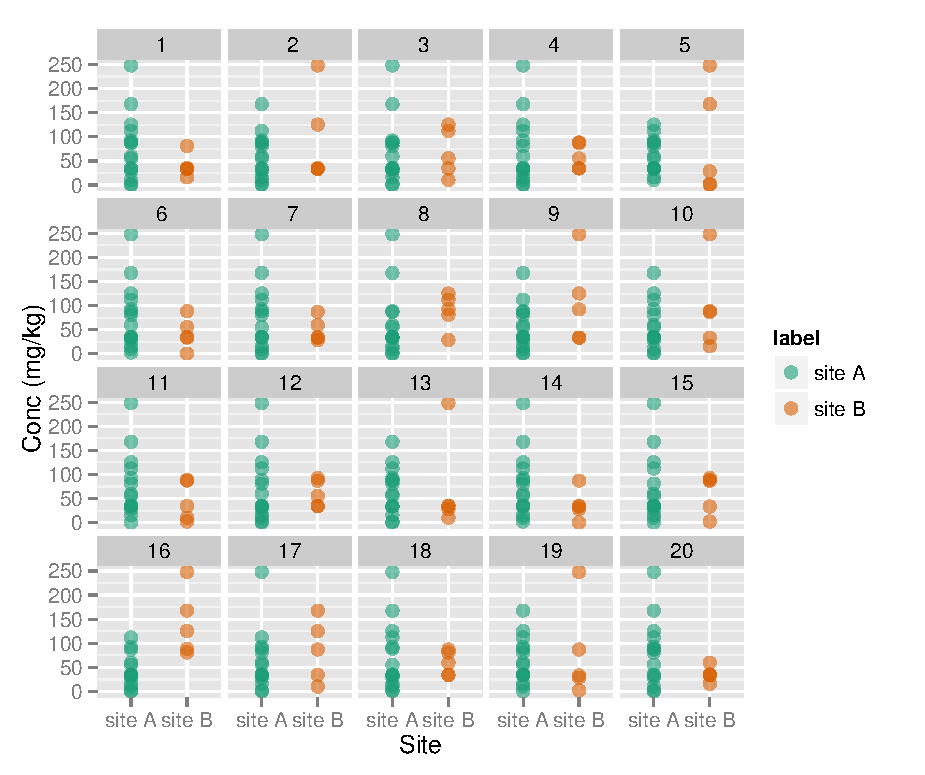
\includegraphics{lineup-dot-rev.pdf}}
      \caption{A typical lineup  ($m = 20$) for testing $H_o: \mu_1 =  \mu_2$. 
      When the alternative hypothesis is true, the observed data plot should have the largest vertical difference between the centers. Can you identify the observed data plot? The solution to the lineup is provided in the Appendix.}
      \label{lineup}
\end{figure}

\cite{majumder:2013} describes the methods of obtaining the power of the visual test, by combining results from multiple users. For their simulation experiments human observers were recruited through Amazon's Mechanical Turk \citep{turk}. Power of the visual test used in their simulation was also calculated theoretically. Their results suggest that the power of visual statistical inference is comparable to conventional tests in a setting of testing the parameters of linear regression models. The subject specific power of the visual test can also be estimated from the multiple responses data from each human observer, which might help quantify individual visual skills.

 
\section{Dimension reduction}  \label{sec:dimred}

Projection pursuit [e.g. \citep{friedman:1974}]  is used for dimension reduction in our studies. Projection pursuit (PP) finds the most interesting low dimensional projection of high dimensional data by maximizing some criterion of interest, e.g. variance or clustering or group separation. As pointed out in \cite{huber:1985} the most exciting feature of projection pursuit is that it can bypass the curse of dimensionality. 

In classification problems, linear discriminant analysis (LDA) can be used to find a low-dimensional space where the groups are most separated. This corresponds to using the LDA index \citep{lee:2009} in projection pursuit. Let $\bf{X_{ij}}$ be the $p$-dimensional vector of the $j$th observation in the $i$th class, $i = 1, \dots, g, j = 1, \dots, n_i$, $g$ is the number of classes, $n_i$ is the number of observations in class $i$, and $n = \sum_{i = 1}^g n_i$. Let $\overline{\blX}_{i.} = \frac{1}{n_i} \sum_{j=1}^{n_i} \blX_{ij}$
be the $i$th class mean and $\overline{\blX}_{..} =
\frac{1}{n}\sum_{i=1}^g \sum_{j=1}^{n_i} \blX_{ij}$ be the total
mean. The LDA PP index is
\begin{equation}
I_{LDA} ({\blA}) = \left \{ \begin{array}{cc}
                       1-\frac{\big|{\blA}^T\blW{\blA}\big|}{\big|{\blA}^T\big
                                  (\blW + \blB\big){\blA}\big|} &
                       \mbox{ for $\big|{\blA}^T\big(\blW + \blB\big) {\blA}\big| \ne 0$}\\
                       0 & \mbox{for  $\big|{\blA}^T\big(\blW + \blB\big) {\blA}\big| = 0$}
                       \end{array}
               \right.
\end{equation}
where $\blA$ is an orthogonal projection onto a $k$-dimensional space and

\begin{eqnarray}
 \blB&=&\sum_{i=1}^g n_i (\overline{\blX}_{i.} - \overline{\blX}_{..})(\overline{\blX}_{i.}
  - \overline{\blX}_{..})^T
:  \mbox{between-class sums of squares}, \nonumber\\
\blW&=&\sum_{i=1}^g \sum_{j=1}^{n_i} (\blX_{ij} -
\overline{\blX}_{i.})(\blX_{ij} - \overline{\blX}_{i.})^T :
\mbox{within-class sums of squares}.\nonumber
\end{eqnarray}

For HDLSS data, the penalized discriminant analysis (PDA) index \citep{lee:2009} is more robust. Let ${\blX}_{ij}^*$ be the standardized vector of ${\blX}_{ij}$. Then 

\begin{eqnarray}
 \blB^s&=&\sum_{i=1}^g n_i (\overline{\blX}^*_{i.} - \overline{\blX}^*_{..})(\overline{\blX}^*_{i.}
  - \overline{\blX}^*_{..})^T: \hbox{between-class sums of squares of the standardized data}\nonumber\\
\blW^s&=&\sum_{i=1}^g \sum_{j=1}^{n_i} (\blX^*_{ij} -
\overline{\blX}^*_{i.})(\blX^*_{ij} - \overline{\blX}^*_{i.})^T: \hbox{within-class sums of squares of the standardized data }\nonumber
\end{eqnarray}
where $\overline{\blX}^*_{i.}$ is the $i$th class mean of the standardized data and $\overline{\blX}^*_{..}$ is the
total mean of the standardized data, which is 0. The PDA index is defined as

\begin{eqnarray}
I_{PDA}(\blA,\lambda) =
1-\frac{\Big|\blA^T\big\{(1-\lambda)\blW^s+n\lambda\blI_p\big\}
\blA\Big|}
              {\Big|\blA^T\big\{(1-\lambda)(\blB^s +\blW^s)+n\lambda\blI_p\big\} \blA\Big|}\label{PDA3}
\end{eqnarray}
where $\blA$ is an orthonormal projection onto a $k$-dimensional space
and $\lambda \in [0,1)$ is a predetermined parameter. Penalized LDA \citep{witten:2011} is a similar approach.

These indices are available for projection pursuit using the \texttt{tourr} package \citep{tourr:2011} in \texttt{R} \citep{r}. The \texttt{tourr} package produces tours of multivariate data. The package also includes functions for creating different types of tours like grand, guided and little tours, which project multivariate data with $p$ dimensions to 1, 2, 3 or $d$ dimensions where $d \le p$. The guided tour function is used here. The guided tour will converge to a maximally interesting projection. Here, that is a projection where groups show the biggest separation. For this paper we used $d = 1$ or 2.  

\section{Amazon Turk experiments} \label{sec:turk}

Amazon's Mechanical Turk \citep{turk} is a service that enables researchers to employ people to do tasks which computers perform poorly. In exchange for their efforts, the subjects are paid, not substantially, but on the scale of the minimum wage of the USA. For visual inference studies, subjects are typically given a block of ten lineups to evaluate during a job. From this block, one lineup is typically used as a filter, and the remaining lineups produce data for the studies. Because a subject evaluates more than one lineup, and a lineup is evaluated by more than one subject, we obtain some replication in the results upon which to estimate variation. The one filter lineup, in which the observed data plot is markedly different from the nulls, is necessary because Turkers are not manually monitored, and a few attempt to maximize financial gain without taking the exercise seriously. 

For this paper, two Turk studies were run, one for the wasps data, and the other for the simulation study. Turkers are redirected from Amazon to a website which describes the study in detail, provides some practice trials, collects demographic details, and responses. The website of the simulation study is \url{http:/mahbub.stat.iastate.edu/feedback_turk7/homepage.html}.

\section{Wasps application} \label{sec:wasp}

We return to the motivating example. Figure \ref{oligo} suggested that the expression patterns of the wasp groups are different.  The question of interest is ``Is this separation real?'' This can be investigated by testing the hypothesis: 

\begin{quote}
$H_o$: There is NO difference in the expression levels between the types of wasp.\\
$H_a$: At least one of the types of wasps has different expression levels.
\end{quote}
A lineup is made of the wasp data obtained from \cite{toth:2010} to test $H_o$ where the null plots are made by permuting the wasp type label, and re-doing the LDA. If there is a real difference between the expression levels for the types of wasps then the observed data plot should be detectable in the lineup. Figure \ref{toth_lineup} shows a lineup.  Three different lineups were created using this procedure. 

\begin{figure*}[hbtp]
%\begin{figurehere}
   \centering
       \scalebox{1.00}{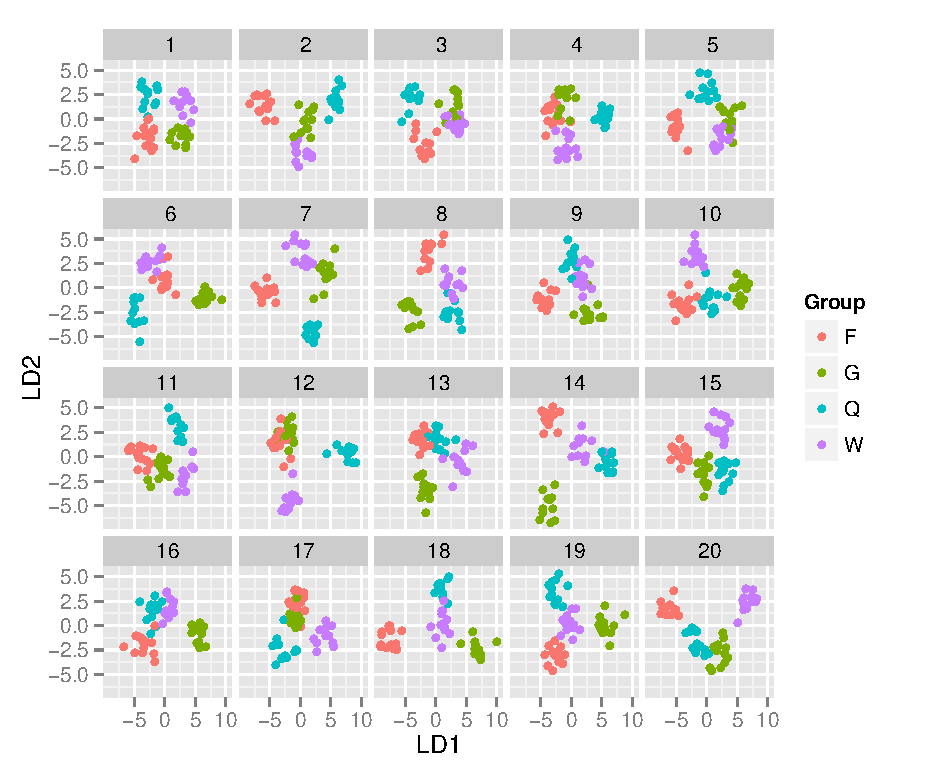
\includegraphics{lineup-wasp-8.pdf}}
       \caption{Lineup of the wasps data. One plot shows the observed data and the remaining 19 show null data where the wasp type labels were randomly assigned. Each plot was produced by conducting LDA on the 40D data to produce the 2D projection with best separation. Which plot shows the most separation between the 4 groups? The solution is provided in the Appendix.}
       \label{toth_lineup}
\end{figure*} 

In addition, three more lineups are made containing only null plots, with one plot randomly chosen to act as an observed data plot. These lineups were shown to the subjects recruited from Amazon Turk.  A total of 116 subjects evaluated the 6 lineups. Table \ref{wasp} shows the results. The detection rate for the plot of the wasp data is 0! This is worse than that of purely noise data. You will notice that for one of the purely noise lineups, subjects very often detected the (random) observed data plot. This happened because the randomly generated observed data plot actually had more separation than any other plot in that lineup. This is the nature of randomness, but makes for interesting results here. The $p$-value is calculated according to the procedure given by \cite{majumder:2013}. The large $p$-values indicate that there is no statistically significant evidence upon which we reject the null hypothesis. Thus we have to conclude that the separation in the wasp data (\cite{toth:2010}) is not real. It is purely the effect of high dimensionality. 

\begin{table}[ht]
\begin{center}
\caption{Results of the Turk study on the wasps data. Detection rate for each lineup is shown, with the number of subjects, and $p$-value associated. The detection rate is highest for one of the purely noise lineups, which occurred because the plot with the most difference between groups happened to be the one that is randomly generated as the ``real'' data. Averaging the $p$-values for each set of lineups, for the wasps is 1.0, and for the pure noise, is 0.67 suggesting that the apparent separation in the wasp data (\cite{toth:2010}) is consistent with pure noise induced by the high dimensions.}
\vspace{0.15cm}
\begin{tabular}{r|r|r|rr}
\hline
  \hline
 Data & Replicate & Num Subjects & Detection rate & $p$-value\\ 
  \hline
  & 1 & 25 & 0.0000 &  1.0000\\
Wasps & 2 & 13 & 0.0000 &  1.0000\\ 
 & 3 & 27 & 0.0000 &  1.0000\\
 \hline
 & 1 & 19 & 0.2632 &  0.0002\\
Purely noise & 2 & 18 & 0.0000 &  1.0000 \\ 
 & 3 & 14 & 0.0000 &  1.0000\\
   \hline
\end{tabular}
\label{wasp}
\end{center}
\end{table}

The probability of separation by chance between two groups in purely noise data, given a fixed sample size and dimension,  was quantified by \cite{ripley:1996} (Proposition 3.1). Figure \ref{dist_1d} illustrates this result for 1D projections, for different $p$, where sample size is fixed at $n = 30$. When $p = 2$, $\hbox{P(separation}|n = 30, p = 2) = 0$ and it reaches 1 when $p = 25$. For data of the size of the wasps, $n = 50$ and $p = 38$, the probability of obtaining separation with only two groups is 1, so we would expect that there would certainly be separation between four groups in 2D.

\begin{figure}[htbp]
\centering
\mbox{\subfigure[P(sep$|n,2$) = 0.00]{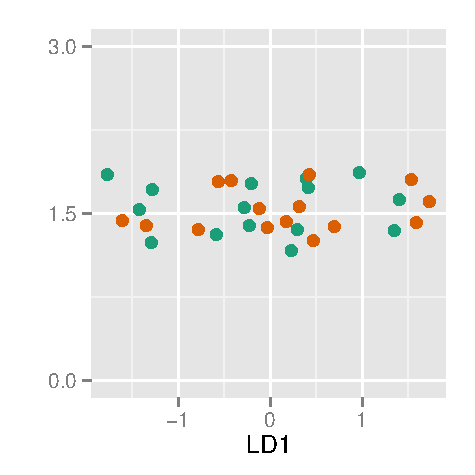
\includegraphics[width=1.1in]{noise-2-rev.pdf}}\quad
\subfigure[P(sep$|n,8$) = 0.01]{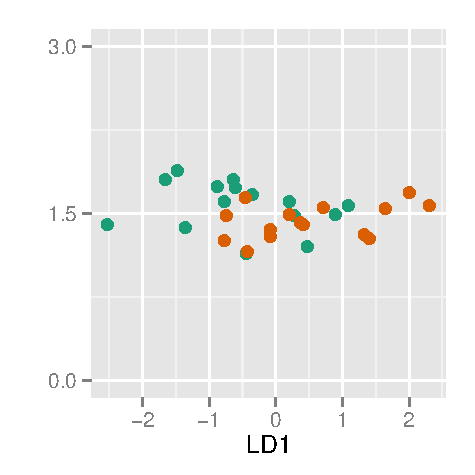
\includegraphics[width=1.1in]{noise-8-rev.pdf} }\quad
\subfigure[P(sep$|n,15$) = 0.64]{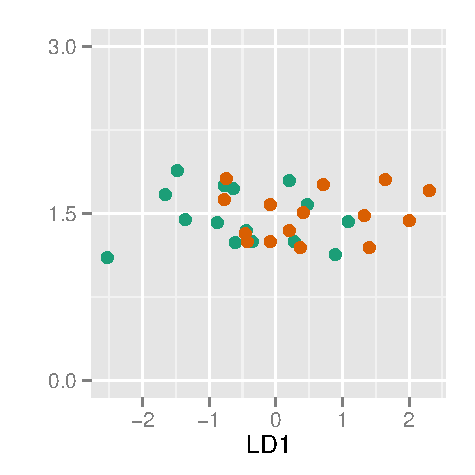
\includegraphics[width=1.1in]{noise-15-rev.pdf} }\quad
\subfigure[P(sep$|n,22$) = 0.99]{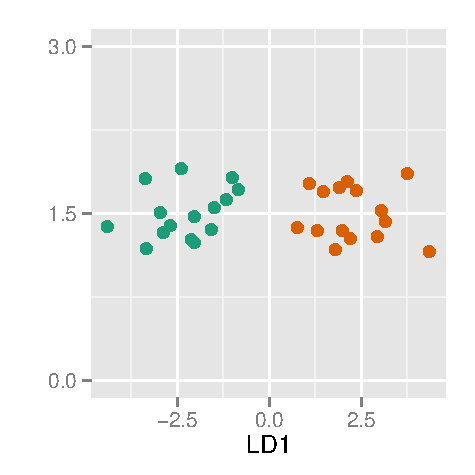
\includegraphics[width=1.1in]{noise-22-rev.pdf} }\quad
\subfigure[P(sep$|n,28$) = 1.00]{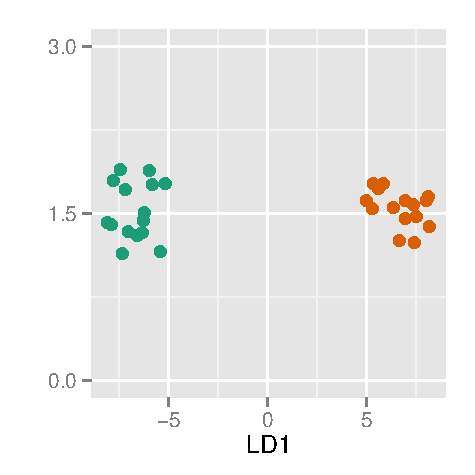
\includegraphics[width=1.1in]{noise-28-rev.pdf} }}
\caption{Plots showing example 1D projections for $p=2, 8, 15, 22, 28$ and $n = 30$ for purely noise data. The probability of obtaining a projection where groups are separated is calculated and displayed below the plots. Of course, once a projection is computed the groups are either separated or not - the event occurred or didn't - and we can see that the last two plots display separated groups. The difference between the groups increases as $p$ increases, and the likelihood of obtaining a projection with separation increases.} 
\label{dist_1d}
\end{figure}

In the original paper \citep{toth:2010}, the dimensionality was reduced from 389 by choosing the genes that showed the greatest separation. So the problem of high dimensionality is actually even worse for these data. In general, reducing the data dimensions so that the sample size is bigger than dimension is not, on its own, sufficient. It is important, even, with so few cases to do cross-validation, or break the sample into training and test sets before conducting analysis. LDA is known also to be a problem for HDLSS data, because it requires estimating more parameters than the available data allows. A better prospect for dimension reduction is the penalized discriminant analysis (PDA) index \citep{lee:2009}, which helps adjust for the over-estimation. Other results and the overall conclusions in \cite{toth:2010} are not affected by the inadequacy revealed by this visual inference analysis. A similar LDA performed on wasp gene expression data with a much higher sample size in \cite{toth:2007} did not suffer from the HDLSS problem. We determined that there were robust separations between the groups based on those data (results not shown).


\section{Follow-up simulation experiment} \label{sec:experiment}

\subsection{Experimental design}

The goal is to determine how well people can detect the presence of real separation as distinguishable from random noise. To achieve this, the experiment is set up with several factors: real separation or pure noise, data dimension and projection dimension. Real separation is achieved by setting 1 or 2 variables with real separation among a number of noise variables.  Sample size is fixed to keep the experiment manageable. Also mean difference is kept fixed. The levels of the factors used in the experiment are given in Table \ref{freq}. Three replicates at each level are generated. These produced 60 different ``observed data sets'', and thus, 60 different lineups. 

\begin{table}[htbp]
\begin{center}
\caption{Levels of the factors used for the simulation experiment.}
\begin{tabular}{cccp{2.2cm}|c}
  \hline
  \hline
  $n$ & projection($d$) & separation & dimension ($p$) & replicates\\
  \hline
  30 & 1 & Yes & 20, 40, 60, 80, 100 & 3 \\
      & & No & 20, 40, 60, 80, 100 & 3\\
   30 & 2 & Yes & 20, 40, 60, 80, 100 & 3 \\
     & & No & 20, 40, 60, 80, 100 & 3\\   
      \hline
\end{tabular}
\label{freq}
\end{center}
\end{table} 

\subsection{Simulation process}

Two groups of $p$ dimensions of data with 15 observations in each group are generated from $N(0, 1)$.  The data from the first group is labeled as group 1 and the data from the second group as group 2, yielding a $30 \times (p + 1)$ matrix, ${\blX}$, where the first 15 observations are from group 1 and the last 15 observations are from group 2. The data for both the groups is purely noise, having no dependence on the groups. So ${\blX}$ can be written as
$${\blX}^{n \times (p + 1)} = ({\blX}_1, {\blX}_2, \dots, {\blX}_p, \hbox{Group})$$ where each ${\blX}_i$ is a vector of dimension 30 for $i = 1, \dots, p$. This matrix ${\blX}$ excluding the Group variable gives the $p$-dimensional pure noise data or data with no separation.

To introduce real separation in the data, values for $p$-th variable ${\blX}_p$ are shifted apart by 6 units between the two groups: 
$$
{\blX}_p = \left\{ \begin{array}{rl}
 {\blX}_p - 3 &\mbox{ if $ {\blX}_p \in$ group 1} \\
 {\blX}_p + 3 &\mbox{ if $ {\blX}_p \in$ group 2}
       \end{array} \right.
$$
and then standardized to have unit variance again. %Hence two sets of data are obtained, each with $p$ dimensions with $n = 30$ observations in each dimension divided into two groups. One of the datasets is pure noise and the other has some real separation in the $p$-th dimension. 
On each dataset of $p$ dimension, a projection pursuit optimization with the PDA index is performed to obtain the 1D projection of best separation, yielding $\blY = \blX \blA$.  

The above procedure is effectively the same for 2D projections with few key differences. The first 10 observations are labelled group 1, the second 10 observations as group 2 and the last 10 as group 3.  So, collectively,  ${\blX}$ can be written as
$$ {\blX}^{n \times (p + 1)} = ( {\blX}_1,  {\blX}_2, \dots, {\blX}_p, \hbox{Group})$$ where each $ {\blX}_i$ is a vector of dimension 30 for $i = 1, \dots, p$. This matrix ${\blX}$ excluding the Group variable gives the $p$-dimensional noise data or data with no separation with 3 groups.

To introduce real separation, the means of the 3 groups are adjusted in the last two dimensions i.e. $ {\blX}_{p-1}$ and ${\blX}_p$. The adjustment is done in the following way:
$$
( {\blX}_{p-1},  {\blX}_p) = \left\{ \begin{array}{rl}
 ( {\blX}_{p-1} - 3,  {\blX}_p) &\mbox{ if $( {\blX}_{p-1},  {\blX}_p) \in$ group 1} \\
 ( {\blX}_{p-1} + 3,  {\blX}_p) &\mbox{ if $({\blX}_{p-1},  {\blX}_p) \in$ group 2} \\
 ( {\blX}_{p-1} ,  {\blX}_p + \sqrt{27}) &\mbox{ if $( {\blX}_{p-1},  {\blX}_p) \in$ group 3}
       \end{array} \right.
$$
and standardized. If $ {\blX}_{p-1}$ versus ${\blX}_p$ are plotted in a scatterplot, the points cluster along the vertices of an equilateral triangle of side 6. Hence the data with 2 dimensions of real separation divided into 3 groups is obtained. A projection pursuit with a PDA index is performed to obtain the 2D projection of best separation, yielding ${\blY} = {\blX}{\blA}$. 

\subsection{Producing lineups}

Two different visual test statistics, $V_1({\blY})$ and $V_2({\blY})$ are used in this paper, for representing 1D and 2D data. $V_1({\blY})$ is a horizontal jittered dot plot, with color representing groups. $V_2({\blY})$ is a scatterplot with color representing groups. Symbols are kept constant for uniformity of appearance. Figure \ref{fig3} shows the two different visual test statistics.

\begin{figure}[htbp]
\centering
\mbox{\subfigure[$V_1({\blY})$]{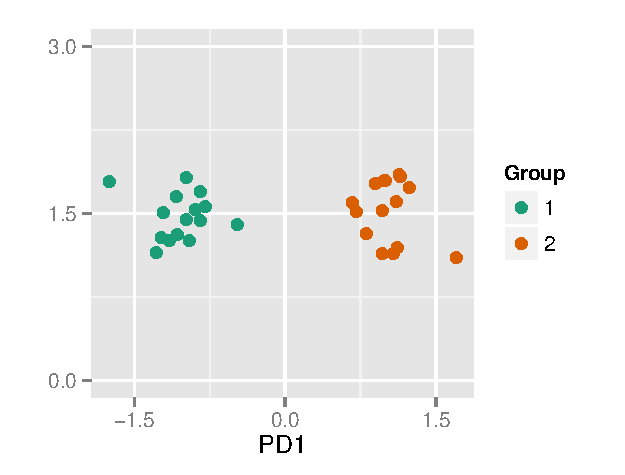
\includegraphics[width=2.5in]{test_statistic_1-rev.pdf}}\quad
\subfigure[$V_2({\blY})$]{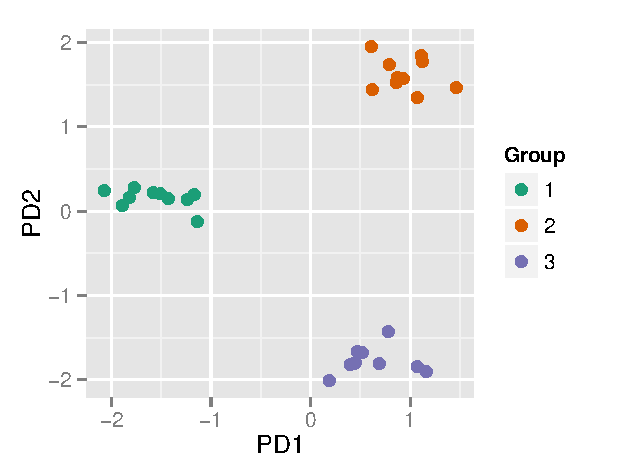
\includegraphics[width=2.5in]{test_statistic_2-rev.pdf} }}
\caption{The visual test statistics $V_1({\blY})$ and $V_2({\blY})$ used.  $V_1({\blY})$ is a horizontal jittered dot plot while $V_2({\blY})$ is a scatterplot of the first and second dimensional projections, with color representing groups in both cases. } 
\label{fig3}
\end{figure}

To obtain the null plots in a lineup, the group variable is permuted in order to break any dependence between the group variable and the other variables. Projections are obtained and plotted in the same way as the test statistic. The test statistic, which is the observed data plot, is placed randomly among the 19 null plots. To maintain the same orientation of the two groups in the 1D projection lineup,  the mean of the projections for each group is calculated for each plot in the lineup and the group with the lower mean is considered to be group 1 and the other group 2. Figure \ref{fig:test_category_1d} shows an example lineup having treatment levels $p = 20$, separation = Yes and $d = 1$. Similarly, Figure \ref{fig:test_category} shows an example lineup for $p =100$, separation = No and $d = 2$.

A statistic measuring the ratio of the average distance within clusters to the average distance between clusters \citep{hennig:2010}, called WBratio, is calculated for each plot in the lineup of both 1D and 2D projections. An additional statistic Wilk's $\lambda$ [e.g. \citep{JW02}] is calculated for 2D projections. To account for the occasional lack of convergence of the projection pursuit optimization, 30 null plots are generated. The 19 null plots which have the smallest Wilk's $\lambda$ values are used for the lineup. 

\begin{figure}[hbtp]
%\begin{figurehere}
   \centering
       \scalebox{1.00}{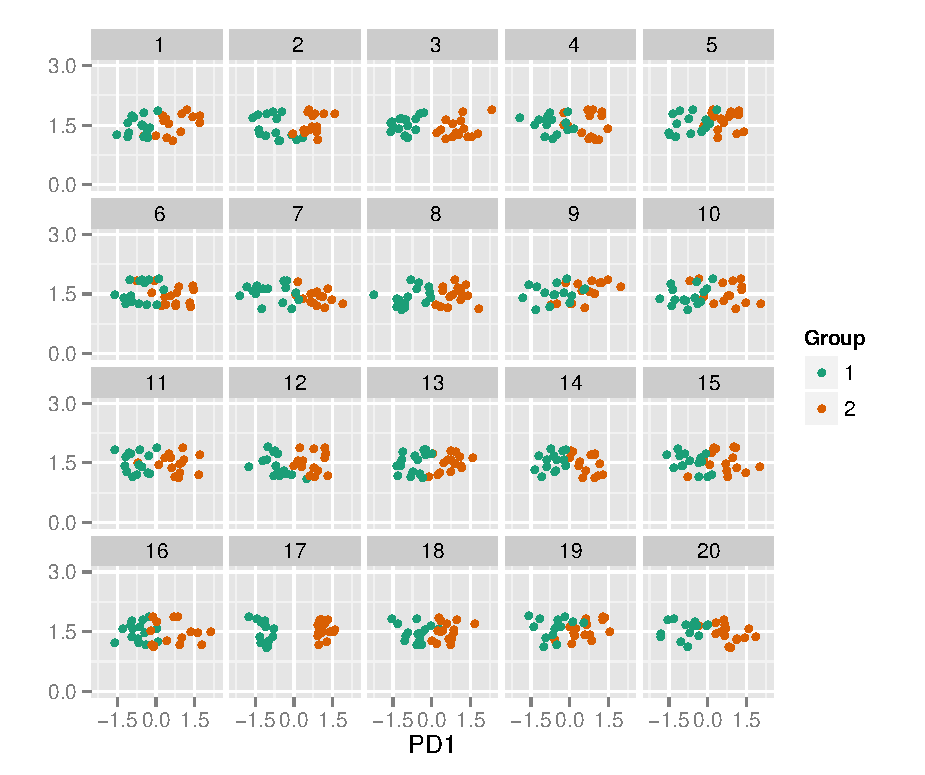
\includegraphics{lineup-20-real-1-17-rev.pdf}}
       \caption{Lineup  ($m=20$) from treatment with $p = 20$, separation = Yes and $d = 1$. The subjects were asked to identify the plot with the most separated colors. Can you identify the observed data plot? The solution to the lineup is provided in the Appendix. }
     \label{fig:test_category_1d}
\end{figure}


 
\begin{figure}[hbtp]
%   \centering
       \scalebox{1.00}{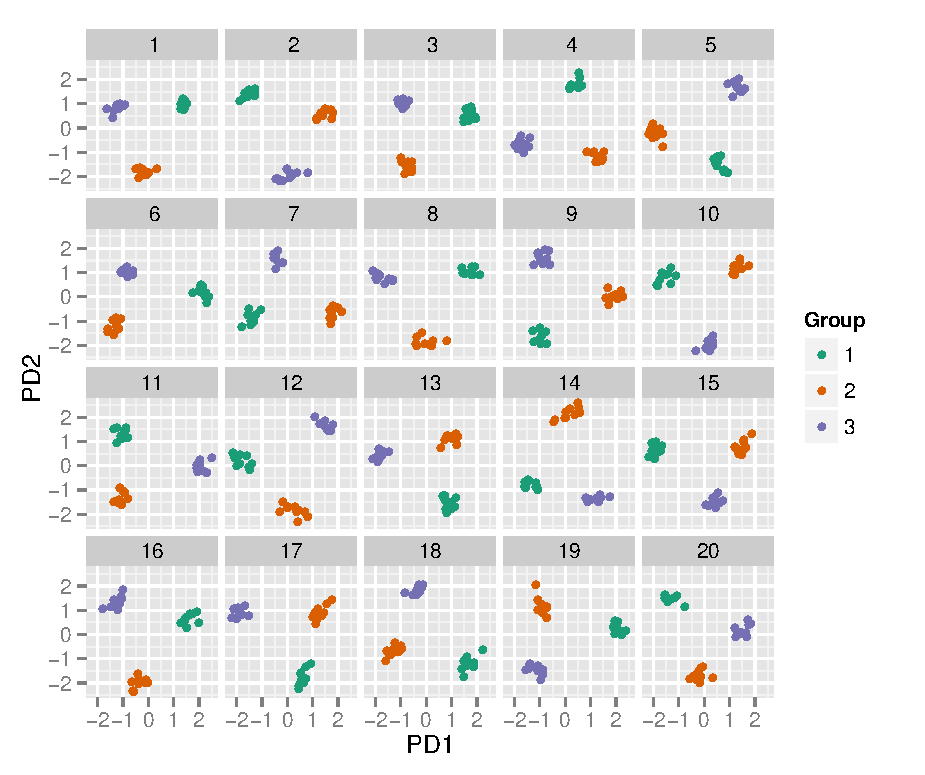
\includegraphics{lineup-100-noise-2-20-rev.pdf}}
       \caption{Lineup  ($m=20$) from treatment with $p = 100$, separation = No and $d = 2$.The subjects were asked to identify the plot with the most separation between the colored groups. Can you identify the observed data plot? The solution is provided in the Appendix. }
       \label{fig:test_category}
\end{figure}

%\ppp

\subsection{Data collection}

Subjects  for the experiment were recruited through Amazon's Mechanical Turk  \citep{turk}. 
%Amazon's Mechanical Turk is a medium that enables researchers to use human intervention to do tasks which the computers are unable to perform currently. In exchange of their efforts, the subjects were paid, not substantially, but on the scale of the minimum wage of the USA.  
Each subject was shown a block of ten lineups. They were asked to identify the plot which has the most separation between the colored groups. Their response was recorded along with a reason for their choice of the plot and the level of confidence they have in their decision.  Gender, age, educational level and the geographic location of each subject were also noted. In total, 1137 lineups were evaluated by 103 subjects, from different locations across the globe. 

%\subsection{Data cleaning}

Each subject was given a very easy lineup (a lineup with $p = 10$ dimensions with some real separation) in the block of ten. Data from subjects who failed to give a correct response to this lineup are removed from the study. If their response to this lineup was correct, data for this lineup was removed but responses for the remaining nine were kept for analysis. This produced 66 lineups evaluated by 101 subjects for analysis.


\section{Results} \label{sec:results}

\subsection{Effect of experimental factors on detection rate} \label{effects}

We would expect that subjects detect the observed data plot more often when there is real separation but that the detection rate diminishes as dimension increases. This is indeed the case, as illustrated by Figure \ref{suc-rate-glm}. The detection rate is plotted against data dimension ($p$), faceted by the levels of separation and projection. The three dots for each $p$ represent the three replicates for each treatment. In a few cases, the dots overlap as the detection rate is same for the replicates. For example, when projection = 1D, dimension = 100 and separation = No, the detection rate is 0 for all the replicates and hence a single dot is shown. Alpha-blending is used on the plots so these ties are darker dots. The line shows the fixed effects from a logistic regression model fitted to the data. The detection rate is higher for small $p$, and on average decreases as $p$ increases, with both 1D and 2D projections for real separation. For purely noise data, the detection rate is effectively flat across $p$, always less than 0.1 on average. Interestingly, the detection rate is higher for data where separation exists than for pure noise, even at $p = 100$, at 0.25 vs 0.05. For real separation, there also appears to be increasing variance as $p$ increases, which is intriguing, too: it might be indicative of the increase in unexplained variance associated with the reduction to low dimensions from the increasingly higher $p$, and the sparsity of space.

\begin{figure}[ht]
%\begin{figurehere}
   \centering
       \scalebox{0.6}{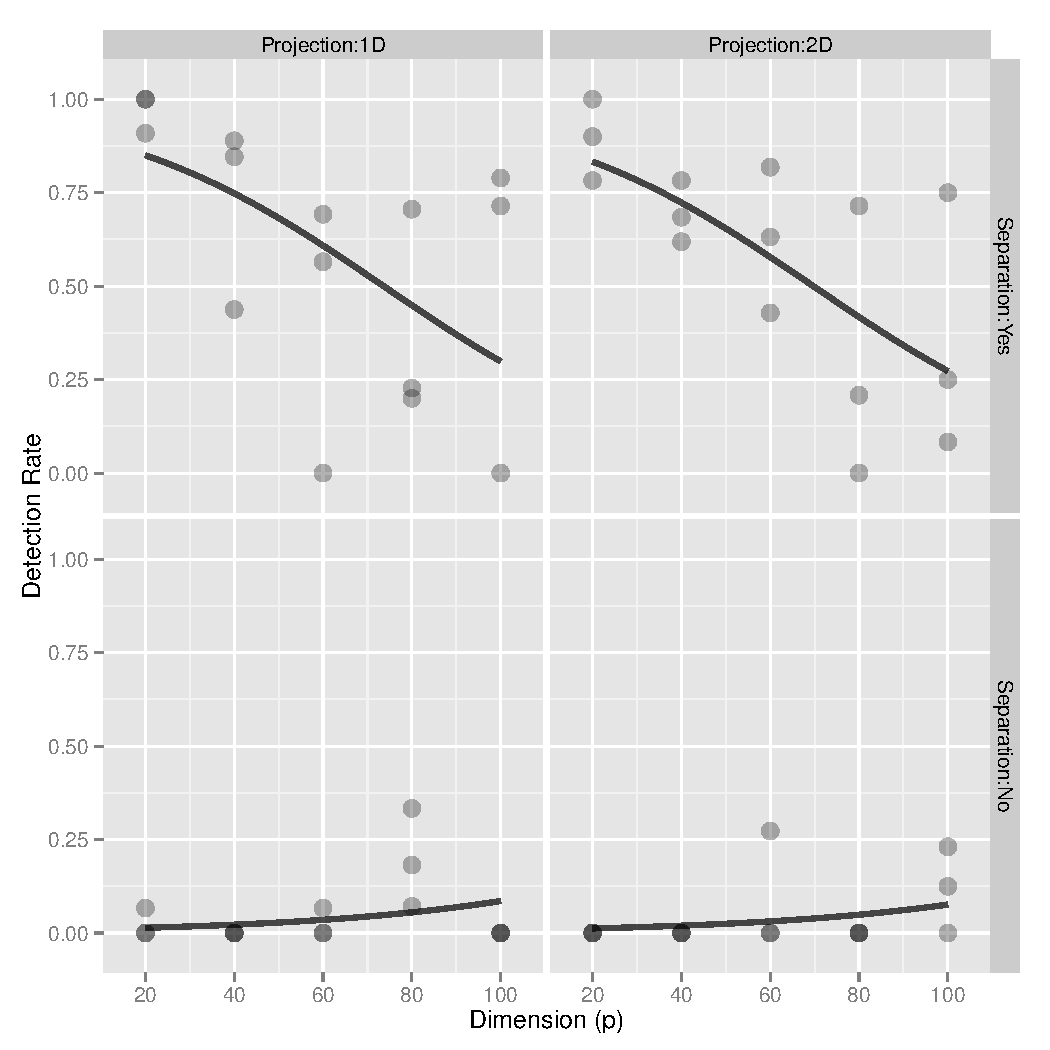
\includegraphics{detection-rate-rep-int-glm-rev.pdf}}
%        \scalebox{0.80}{\includegraphics{result-noise.pdf}}
      \caption{Detection rate by dimension, faceted by projection and separation. The three points represents the three replicates for each treatment level. A fixed effects logistic regression model is overlaid on the points. It can be seen that the detection rate decreases as $p$ increases for data with real separation. When the data is purely noise data, the detection rate is flat across dimensions. Detection rate does not change with projection.  Even with $p = 100$ subjects more often detected separation than would be expected by chance. }
       \label{suc-rate-glm}
\end{figure}

Table \ref{params} shows the estimates of the parameters from the fixed effects logistic regression model, the standard errors and the corresponding $p$-values. We observe that the $p$-values corresponding to dimension and presence of real separation is very highly significant. However, the $p$-value corresponding to the projection is large, which suggests that the difference between 1D and 2D projections is not significant. One of our concerns with the 2D projections is that the rotation of the group was not adjusted, and that this might diminish the subjects ability to identify the observed data plot. The lack of significant difference between 1D and 2D results suggest that rotation was not important. The interaction term is also significant, which says that the detection rate changes in the presence or absence of separation -- detectability of the observed data plot decreases with dimension when there really is separation.

\begin{table}[ht]
\begin{center}
\caption{Table summarizing results of experiment. Columns correspond to the estimate, the standard error and the $p$-value of the parameters used in logistic regression model. As dimension ($p$) increases, detection of separation decreases. Subjects can detect the separation if it exists even when $p = 100$. Subjects were equally good in 1D or 2D projections.}
\vspace{0.15cm}
\begin{tabular}{r|rrr}
\hline
  \hline
 Parameters & Estimate & Std. Error  & $p$-value \\ 
  \hline
Intercept  & 2.381 & 0.278  & 0.000 \\ 
  dimension($p$) & $-$0.032 & 0.004  & 0.000 \\ 
  separation = No & $-$7.097 & 0.911  & 0.000 \\ 
  projection = 2D & $-$0.127 & 0.181  & 0.483 \\ 
  separation:dimension & 0.056 & 0.011 & 0.000\\
   \hline
\end{tabular}
\label{params}
\end{center}
\end{table}

The effect of demographic variables (age, gender and education) on the detection rate was also studied, and found to be insignificant. 

%\subsection{Does rotation in the 2D projections affect the responses?}

%The 1D projections are plotted in a lineup (Figure \ref{fig:test_category_1d}) making the adjustment that the group with the lower values of projection are always considered to be group 1. So the orientation of the groups does not affect the response of the subjects. But in case of 2D projections, the groups are rotated in a different way in each plot in the lineup (Figure \ref{fig:test_category}) which may influence the response of the subjects. We can check if the rotation in the 2D projections does effect the performance. Since the 1D projections are adjusted, the lineups of the 1D projections are used as a control and the responses for the 1D and 2D projections are compared. Figure \ref{suc-rate-glm} shows that there is not much of a difference between the 1D and 2D projections both in presence and absence of real separation. This is also verified in Table \ref{params} where the effect of the projections is not significant at 5\% level.  

%\newpage

\subsection{Time taken to respond under different treatments}

We would expect that the amount of time taken to respond will increase with the difficulty of identifying the observed data plot in a lineup. Figure \ref{time-taken} shows the time taken in seconds to respond (on a log scale) by $p$, facetted by projection. Color indicates presence or absence of separation. The line shows the trend over dimension. Bootstrap resampling bands (\cite{buja:2005}) are overlaid, which effectively provide confidence bands for the curves. Notice that,  when the data has some real separation (green), as the dimension increases on average,  subjects take more time to respond to the lineups. But when the data is purely noise (brown), the increase of dimension does not have any effect on the time taken. This suggests that as the number of dimensions increases, it becomes harder to spot the observed data plot among the null plots. On the other hand, the difficulty of spotting the observed data plot for a data with purely noise does not vary with dimension. It can also be seen that the time taken when the data is purely noise is overall higher than the time taken when the data has some real separation. The bootstrap resampling bands suggest that there is only significantly reduced time taken when $p=20$ or $40$. 



\begin{figure*}[hbtp]
%\begin{figurehere}
   \centering
       \scalebox{0.7}{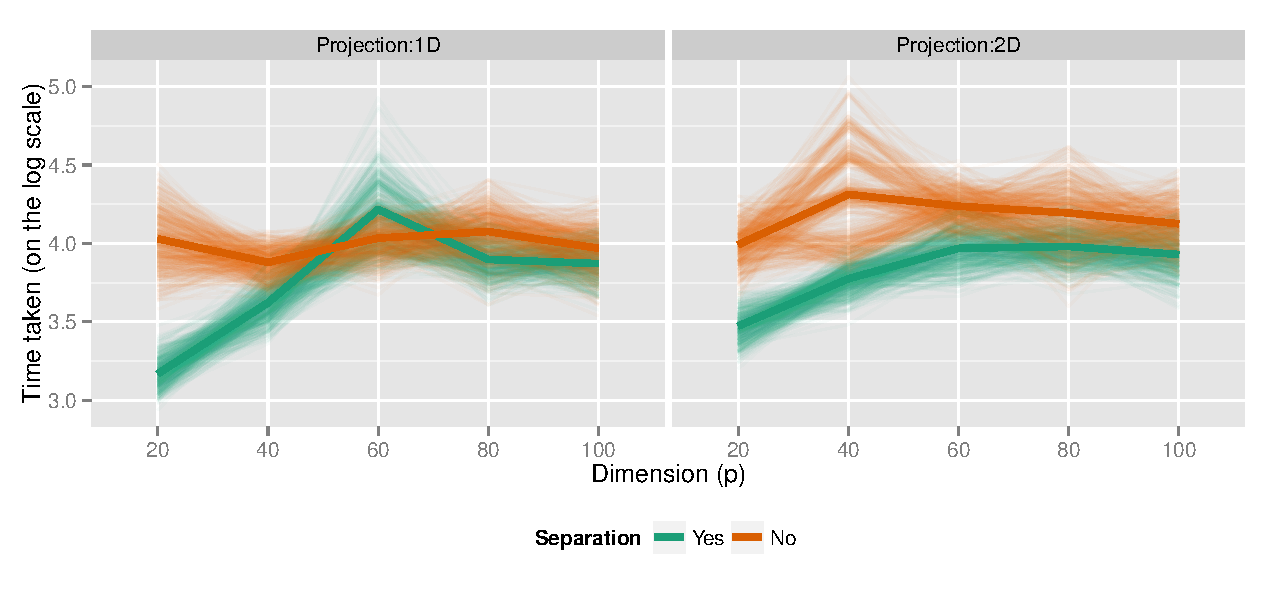
\includegraphics{time-taken-log-bands-1.pdf}}
%        \scalebox{0.80}{\includegraphics{result-noise.pdf}}
      \caption{Time taken in seconds to respond on log scale against dimension colored by separation and faceted by projection. A line shows the trend over dimension for each separation within projection. Bootstrap resampling bands are drawn for each colored lines. Time taken to respond is higher when the data has no separation. Also as dimension increases, the time to answer when there is separation is equal to the time taken when there is no separation. }
       \label{time-taken}
\end{figure*}

\subsection{What affects decisions?}

\normalsize

Figure \ref{sep} examines the subjects choices in detail. The relative frequency of picks of each plot in the lineup is plotted against a measure of average separation between groups. Each cell of this figure shows data from one of the lineups used in the study, 60 in total. Each ``pin'' represents a plot in a lineup, so each cell here has 20 pins, indicating the frequency that the plot was chosen. Red represents the observed data plot. Two separate figures are made for the 1D and 2D projections. The top three rows correspond to data containing real separation between the groups, and for the bottom three rows all of the data is purely noise. Columns indicate dimension ($p$). Replicates are in different rows. The taller the pin the more often that particular plot is chosen from the lineup. We asked subjects to pick the plot where the groups are most separated, and this is effectively what they picked. The plot in each lineup with the largest average separation tends to have the highest frequency. This is more obvious when there is real separation, and also when dimension is small, but it is also seen in the lineups containing pure noise data. This is reassuring -- that subjects did well at detecting the biggest difference.  
%For some of the lineups though, the choices are a little surprising, for example separation = No, dimension = 60, rep = 2, projection = 2D. Investigating these lineups further may reveal why this is. (See supplementary material).

\begin{figure}[htbp]
\centering
\mbox{\subfigure[Projection:1D]{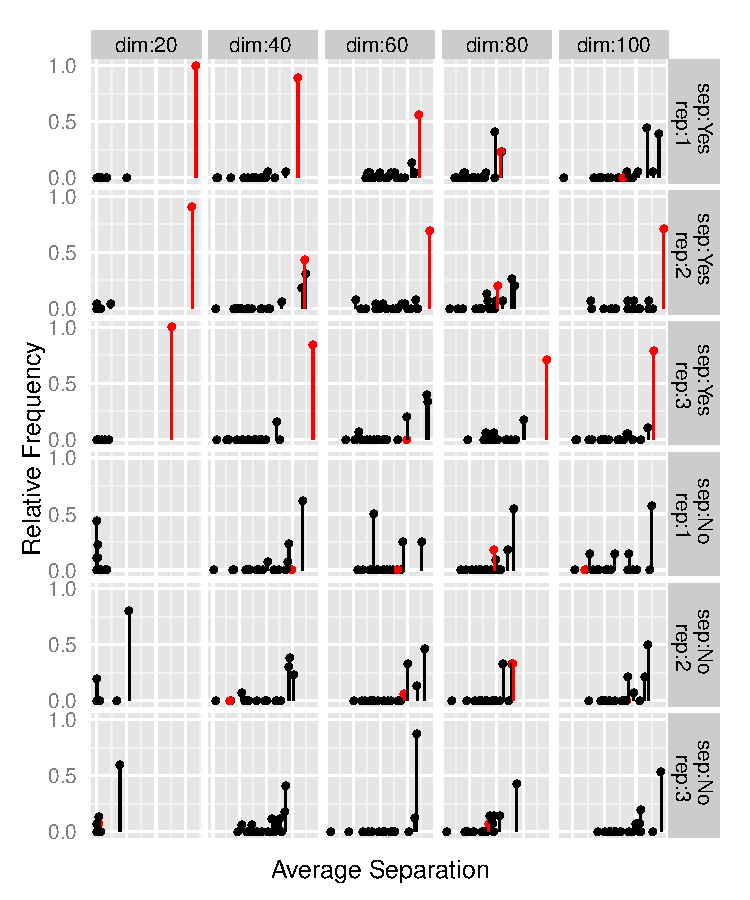
\includegraphics[width=3in]{avg-sep-1.pdf}}\quad
\subfigure[Projection:2D]{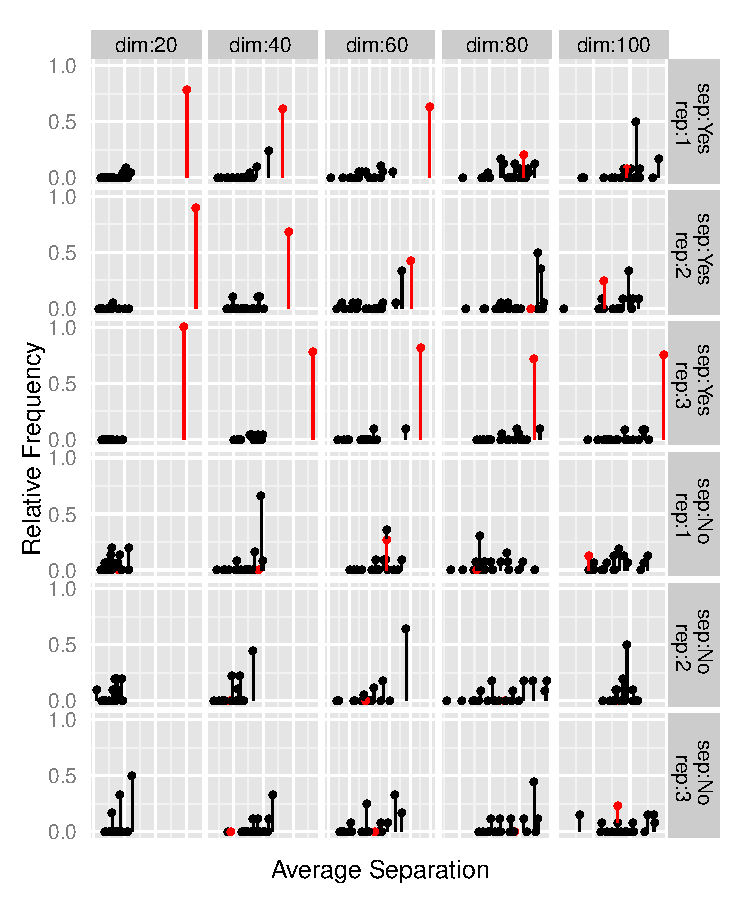
\includegraphics[width=3in]{avg-sep-2.pdf} }}
\caption{Comparing the choices that subjects make for each lineup. Relative frequency of plots chosen against a measure of the average separation between groups, the larger the value the more separated are the groups. Each cell here shows the data for one of the lineups used in the experiment, 60 in total, and each ``pin'' represents a plot in the lineup, 20 for each lineup. Red indicates the observed data plot. Subjects are asked to pick the plot in the lineup where the groups are the most separated, so we would expect that more subjects would pick the plots with the largest average separation. In general, this happens, the tallest pins are in the right of each cell. The top three rows show the results for the data with separation, so the observed data plot (red) is typically the pin on the very left of the cell, less so for the higher dimensions which are the cells at right. Figure (a) shows 1D projections and Figure (b) shows for 2D projections. There is not much difference between the two figures. } 
\label{sep}
\end{figure}

\subsection{How do the null plots affect choices?}

We have learned that subjects tend to pick the plot in the lineup that exhibits the most separation.  Because visual inference only allows for a finite (small) number of comparisons against the sampling distribution, the influence of the null plots in the lineup on the observer's choice is important. If any null plot has a strong signal, subjects may choose this plot over the observed data plot. To gauge the influence of the null plots, we first calculate the average separation between the clusters in each plot of the lineup. For each lineup we then calculate the difference between the maximum average separation of the null plots and the average separation for the observed data plot for each lineup. Figure \ref{null} examines the influence of the null plots on this pick. The detection rate and mean time taken in seconds are plotted against difference. The vertical line is a reference line where the difference is 0 -- the value at which the observed data plot has the same signal as the most extreme null plot. The points to the right of the line should indicate easier lineups and those to the left indicate more difficult lineups in the sense that the null plots have more signal than the observed data plot. We can see that as the difference increases, the detection rate increases and also time taken to choose decreases, suggesting easier lineups. More details on the measurement of the influence of the null plots are available in \cite{roychowdhury:2012}.

\begin{figure}[htbp]
\centering
\subfigure[Projection:1D]{
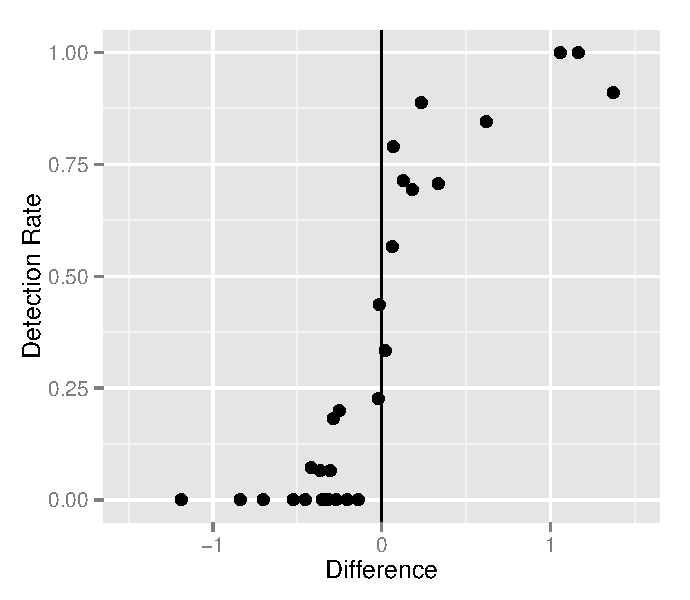
\includegraphics[width=3in]{detection-diff-avg-sep-1.pdf}
}
\subfigure[Projection:2D]{
\includegraphics[width=3in]{detection-diff-avg-sep-2.pdf}
}
\subfigure[Projection:1D]{
\includegraphics[width=3in]{mtime-diff-avg-sep-1.pdf}
}
\subfigure[Projection:2D]{
\includegraphics[width=3in]{mtime-diff-avg-sep-2.pdf} 
}
\caption{Detection rate and mean time taken to respond in seconds are plotted against the difference for 1D and 2D projections separately. The difference is between maximum separation of all the null plots and separation of the observed data plot for each lineup for 1D projections but for 2D projections the difference is based on the average separation between the groups. The vertical line represents difference equal to 1 when the average separation of the observed data plot is equal to the maximum average separation of the null plots for 2D projection. The points left to the line indicates a difficult lineup in the sense that at least one of the null plots had a lower average separation value than the observed data plot. (a) and (b) As difference increases, detection rate increases. (c) and (d) As difference increases,  mean time taken decreases indicating that the subjects have an easier time in identifying the observed data plot. }
\label{null}
\end{figure}

\section{Conclusions}

The results of applying visual inference procedures to classification problems on HDLSS data suggest that visual inference may be effective for improving the understanding of the emptiness of space in this type of data. With visual inference we saw that people can visually detect real separation as different from noise up to a reasonably high dimension, for 1D and 2D projections. Visual inference provides a calibration for reading the separation. 

We also learned from visual inference, although didn't discuss this in the paper, that the projection pursuit optimization procedure in \texttt{tourr} package is performing correctly. It is possible that visual inference might be used to calibrate results of similar algorithms, where the optimization is used to yield visual products, like multidimensional scaling, PCA, independent component analysis (ICA) (\cite{comon:1994}) and local linear embeddings (\cite{roweis:2000}).

There are several natural next steps for this research. One is to examine the possibility of using visual inference to obtain confidence bands for the value of $p$, where separation is certain, for fixed sample size and dimension, particularly if a component of real separation is included. Another direction is to build metrics to quantify the difficulty of a lineup and the influence that null plots have on identifying the data plot. It may be useful to incorporate the approaches into the statistics curriculum, particularly elementary statistics and applications areas such as gene expression analysis, to improve understanding of randomness. 



\section*{Acknowledgement}
%
This work was funded by National Science Foundation grant DMS 1007697. All figures were made using the R \citep{r} package ggplot2 \citep{hadley:2009}.





% Article top matter
%\title{Where's Waldo : Measuring the quality of a lineup}
%\title{Where's Waldo: Looking closely at a Lineup}
\chapter{UTILIZING DISTANCE METRICS ON LINEUPS TO EXAMINE WHAT PEOPLE READ FROM DATA PLOTS}\label{ch:metrics}
\vspace{0.8cm}
\begin{center}
\large{A paper to be submitted to \it{Journal of Computational and Graphical Statistics}.}

\large{Niladri Roy Chowdhury, Dianne Cook, Heike Hofmann, Mahbubul Majumder, Yifan Zhao}\\

\end{center}
%\maketitle

\section*{Abstract} 
Graphics play a crucial role in statistical analysis and data mining. This paper describes metrics developed to assist the use of lineups for making inferential statements. Lineups embed the plot of the data among a set of null plots, and engage a human observer to select the plot that is most different from the rest. If the data plot is selected it corresponds to the rejection of a null hypothesis. Metrics are calculated in association with lineups, to measure the quality of the lineup, and help to understand what people see in the data plots.  The null plots represent a finite sample from a null distribution, and the selected sample potentially affects the ease or difficulty of a lineup. Distance metrics are designed to describe how close the true data plot is to the null plots, and how close the null plots are to each other. The distribution of the distance metrics is studied to learn how well this matches to what people detect in the plots, the effect of null generating mechanism and plot choices for particular tasks.  The analysis was conducted on data that has already been collected from Amazon Turk studies conducted with lineups for studying an array of data analysis tasks.

%Statistical graphics play a crucial role in exploratory data analysis, model checking and diagnosis. Until recently there were no formal visual methods in place for determining statistical significance of findings. This changed, when \citep{buja:2009} conceptually introduced two protocols for formal tests of visual findings. In this paper we use the lineup protocol \citep{buja:2009} and take a closer look at the null plots that appear in a lineup along with the true plot. Different distance measures between the null plots and the true plot are calculated. On the basis of these distance measures, a measure of ``closeness'' between the null plots and the true plot is defined. A human subjects experiment is conducted using simulated data to provide controlled conditions. Results suggest that some of the distance measures works better than the others in most situations.
%\end {abstract}


%{\color{red} Key Ideas:
% \begin{itemize}
%\item Measure ease of a lineup (? signal strength.)
%\item Distance metric that is universal?
%\item Evaluating distance metrics, incorporating turk study data.
%\end{itemize}}
%\begin{multicols}{2}
%\twocolumn

\section{Introduction} 
Graphics are an important component of big data analysis, providing a mechanism for discovering unexpected patterns in data. Pioneering research by \citet{gelman:2004}, \citet{buja:2009} and \cite{majumder:2013} provide methods to quantify the significance of discoveries made from visualizations. %Although, there have been major advances in statistical graphics over the years, for example, systems like R \citep{R} provide high quality static graphics, and very recently some access to interactive graphics. But the problem remains that graphics are not widely considered to be a part of inferential statistics. 
\cite{buja:2009} introduced two protocols which bridge the gulf between traditional statistical inference and exploratory data analysis. These are the Rorschach and the lineup protocols. The Rorschach protocol helps to understand the extent of randomness. The lineup protocol places a statistical plot firmly in the hypothesis testing framework, where a plot of the data is considered to be a test statistic. Unlike the simpler numeric test statistics in classical inference, though, the plot as a test statistic is a complex entity. This plot is compared with a set of null plots, obtained from an appropriate distribution consistent with the null hypothesis. The lineup protocol places the data plot randomly among the obtained null plots, and requires a human observer to examine the plots and identify the most different plot. If this plot is that of the data, this is quantifiable evidence against the null hypothesis. 

Figure \ref{lineup-example} is an example of a lineup. Suppose we have the following statistical model

$$Y_i = \beta_0 + \beta_1 X_{i1} + \beta_2 X_{i2} + \dots + \epsilon_i$$

\noindent and we are interested in testing the following hypothesis:

$$H_o : \beta_k = 0 \qquad \qquad \hbox{vs} \qquad \qquad H_A: \beta_k \ne 0$$

\noindent where $X_k$ is a continuous covariate. The true plot is obtained by plotting $Y$ against $X_k$ with a regression line overlaid. The null plots are obtained by simulating data from $N(X\hat{\beta}, \hat{\sigma}^2)$ and plotting using the same scatterplot method as the true data. These parameter estimates ($\hat{\beta}, \hat{\sigma}^2$) are obtained by fitting the null model to the true data. The plot of the true data is randomly placed among a set of ($m$ - 1) null plots to produce a lineup of size $m$. The human subjects are then shown this lineup and asked to identify the plot which has the steepest slope. If the human subjects can identify the plot of the true data, we reject the null hypothesis and conclude that there is a significant linear relationship between $Y$ and $X_k$. 

\begin{figure}[htbp]
\centerline{\includegraphics[width=1\textwidth]{lineup-protocol-example.pdf}}
\caption{Lineup plot of size $m = 20$ using scatterplots with regression line overlaid. This tests $H_o: \beta_k = 0$, where covariate $X_k$ is continuous. One of the plots in the lineup is the plot of the true data. The other plots are null plots generated by simulating data from a null model that assumes that the null hypothesis is true. Can you identify the plot with the steepest slope?  }
\label{lineup-example}
\end{figure}

The lineup protocol was formally tested in a head-to-head comparison with the equivalent conventional test by \cite{majumder:2013}. The experiment utilized human subjects from Amazon's Mechanical Turk (\cite{turk}) and used simulation to control conditions. The results suggest that the visual inference is comparable to conventional tests in a controlled conventional setting. This provides support for its appropriateness for testing in real exploratory situations where no conventional test exists. Interestingly, the power of a visual test increases with the number of observers engaged to evaluate lineups, and the pattern in results suggests that the power will provide results consistent with practical significance (\cite{kirk:1996}).

%But there may be one issue when using the lineup protocol. In traditional hypothesis testing, the true value of the test statistic is compared with all possible values of its null distribution. If the statistic is extreme on this scale, there is evidence to disbelieve the null hypothesis. With the lineup protocol, for a data plot to be considered to be extreme, a human judge must pick it as different from the other plots in the lineup. 

%\begin{figure}[htp]
%\centerline{\includegraphics[width=0.5\textwidth]{diagram.pdf}}
%\caption{Decision regions  for classical inference for $H_0: \mu=\mu_0$ vs $H_a:\mu>\mu_0$.}
%\label{classical}
%\end{figure}
%
%\begin{figure}[hbtp]
%%\begin{figurehere}
%   \centering
%       \includegraphics[width=0.5\textwidth]{visual-inference-plot-1.pdf}
%      \caption{Sampling distribution of the test statistic with the true value and the values for the null plots corresponding to the lineup in Figure \ref{lineup}.}
%      \label{visual-plot}
%%	\vspace{-.1in}
%\end{figure}

\begin{figure}[htbp]
\centering
\mbox{\subfigure[Classical Inference]{\includegraphics[width=3in]{diagram.pdf}}\quad
\subfigure[Visual Inference]{\includegraphics[width=3in]{visual-inference-plot-1.pdf} }}
\caption{If the lineup protocol was to be used instead of classical inference this is what it would look like. (a) Decision region (shaded in red) for classical inference for $H_0: \mu=\mu_0$ vs $H_a:\mu>\mu_0$  and (b) values corresponding to the true value (red) and the null plots (blue) in a single lineup of size $m=20$ that would be used to test the same null hypothesis.  The actual  data plot is extreme relative to the null plots, and observers would likely be able to pick it out, resulting in a decision to reject the null hypothesis. In practice, the lineup protocol would not be used if a classical test can be used.} 
\label{compare}
\end{figure}


%{\color{red}***  Point 1: Finite comparison vs infinite comparison, measuring how different data plot is from null plots}

In traditional hypothesis testing, the sampling distribution of a test statistic is functional and continuous. In the lineup protocol, although conceptually we may have an infinite collection of plots from the null distribution, in practice, we can only evaluate against a finite number of null plots. A human judge has a physical limit on the number of plots they can peruse. This poses one of the issues with using the lineup protocol.  Figure \ref{compare} illustrates the difference. In traditional inference, the black curve represents the sampling distribution for the $t$-distribution under the null hypothesis, and the shaded red area shows the rejection region. In visual inference, let us consider that the black curve gives the sampling distribution although the sampling distribution is essentially a distribution of null plots. Although the test statistic is not numeric, the true data plot which is the test statistic is represented using red bar and the null plots that are drawn from the null distribution are the blue bars. % for the plots in the lineup shown in Figure \ref{lineup}. 
Effectively,  in visual inference the red line is compared only to these finite number of blue lines visually to make a decision, unlike classical inference where we look at the rejection region (Figure \ref{compare}) to make decisions. Even though the data plot might be extreme, it is possible by randomly selecting from the null distribution, to obtain a null plot that is more extreme, as Tukey suggested \citep{fernholz03}:

\begin{quotation}
``There [in Tukey's Data Analysis class] I discovered that [...]  a random sample is indeed a ``batch of values'' which ``fail to be utopian'' most of the time.''
\end{quotation}


%{\color{red}***Point 2: Use metrics to ensure that a range of comparisons is made available to observers}

This can be partially solved by having a large number of observers, who each evaluate lineups constructed with different null plots. Having some idea of the type of coverage of the sampling distribution that is provided by the lineups would be useful ahead of engaging observers and evaluating the lineups. Could we say that lineup X is expected to be ``difficult'' but lineup Y is expected to be ``easy'' then it may help in determining an appropriate number of observers? A difficult lineup is one where the data plot is similar to the null plots, and an easy lineup is where the data plot has some feature that makes it very different from the null plots. Being able to compute a plot to plot distance metric would be very helpful ahead of running a lineup protocol.

%Researchers needs to provide a range of comparisons to observers to judge. An efficient design of experiment would be to provide a range of lineup plots with varying difficulty to the human subjects to look at. So far the difficulty of a lineup can be evaluated based on the performance of the subjects. The performance of the subjects can be analyzed after the experiment. But as a researcher, it would be interesting to have an idea about the difficulty of the lineups even before the experiment is conducted so the subjects see a set of lineups with varying difficulty. Distance metrics can be of great help in this case. 


%To avoid basing conclusions on artifacts introduced by a `bad' sample, we need to be aware of properties of this set of null plots. In this paper, we develop techniques that help to determine the quality of the lineup. A variety of distance metrics measuring the ``closeness'' of the true data plot and the null plots, and the null plots with themselves are examined. These are compared to human subject picks in several Amazon Turk studies.  Describing plots numerically, is something  of an oxymoron, it cannot be done. Nonetheless, the distance measures provide indications of the quality of a lineup. The purpose of this paper is to help determine if a lineup might provide inadequate coverage of the full null distribution, and these measures might help to gain more insight on how the human eyes work in reading statistical graphics. 

%{\color{red} ***  Point 3: Metrics might replace human observers, eventually, but as of now, human eye can still beat numbers for finding unexpected patterns. The lineup protocol gives us a chance to evaluate metrics to finding unexpected structures - check out the scagnostics literature}

This is a two way process: As metrics are devised to measure the quality of a lineup, the lineup protocol also provides an opportunity to measure the performance of a metric. The human eye can detect patterns in a plot that just cannot be easily quantified numerically, which is why graphics provide an important tool for exploring data and finding the unexpected. Describing plots numerically, is something  of an oxymoron, it cannot be universally done. An example in past work are scagnostics \citep{tukey:1977,wilkinson2005graph} which were developed to assess the different aspects of scattered points like outliers, shape, trend, density and coherence.  If a scatterplot has just one of these structures the scagnostics are descriptive, however, they fail terribly if a plot contains more than one. The goal here is to find some distance measures that can provide some indications of the quality of a lineup, and then to use the results of observer evaluation to determine which metrics best match what people see.

%{\color{red} *** Point 4: Metrics can help us understand what it is that people pick up on to trigger a detection of the data. Currently lineups rely on people verbally reporting why they picked a plot. }

Following up on choices, observers are asked to describe their reasoning. These reasons are used to obtain more information about the rejection: was it some nonlinear dependency, an outlier, clustering, that triggered the detection of the data plot? Good distance metrics may also help relate the descriptive words used with mathematically defined features. 

The article is organized as follows. Section \ref{sec:null} discusses the null generating mechanisms. Section \ref{sec:meas} defines the distance measures and discusses the choice of the measures. The distribution of the distance measures are studied in Section \ref{sec:distri}. Section \ref{sec:plot_type} describes the effect of the plot type and the question of interest on the distance measure while Section \ref{sec:eval} talks about the distance evaluations. In Section \ref{sec:nbin}, the methods to select the number of bins for the binned distance is described. Section \ref{sec:results} presents a comparison of the distance measures to the performance of human subjects in several experiments conducted by Amazon's Mechanical Turk.


%Any statistical analysis must include some sreftatistical graphics. For exploratory data analysis, statistical graphics play an invaluable role in model checking and diagnostics. Even though we have established mathematical procedures to obtain various statistics, we need to support the results by also producing the relevant plots. 

%In recent times there have been major advances in statistical graphics. Modern computing systems like R and SAS produce high quality statistical graphics. Buja et al. 2009, following from Gelman 2004, proposed two protocols that allow the testing of discoveries made from statistical graphics.

%In this paper we are interested in the quality of a lineup plot. In visual inference, the actual plot is the test statistic and the lineup plot is the null distribution. Unlike classical inference, the null distribution is represented by the 19 null plots that we obtain randomly from the actual plot assuming that the null hypothesis is true. So the decision of rejection or failure of rejection of the null hypothesis is heavily dependent on these 19 null plots. This induces us to take a closer look at the null plots. For this purpose, we calculate different distance matrices between the null plots and the actual plot to get a measure on how close is each null plot to the actual plot. We also calculate the distance matrices between the null plots to see how close are the null plots to each often. Finally a percentile value is calculated to find how often such a distance appears in a lineup and a z-score of the different distances is calculated to get a measure on the closeness between the null plot and the actual plot and also compare between two different lineups.  

%In this paper we presents results of a human-subject study assessing the performance of the different distance matrices. Section \ref{sec:visual_test} describes the basic idea of the visual inference and also gives the definition of the different distance measures. Section \ref{sec:asso} and Section \ref{user.distance} applies these ideas and uses the definitions to calculate the different distance measures. In Section \ref{results} and Section \ref{sec:conclusions} we outline the setup and present results.

%\section{Visual Statistical Inference and Definitions} \label{sec:visual_test} 

%This section outlines the concepts of visual inference in comparison to the procedures of classical statistical inference and also gives the definition of the different distance measures. 

%Let $\theta$ be a population parameter of interest, with $\theta \in \Theta$, the parameter space. 
%Any null hypothesis $H_0$ then partitions the parameter space into $\Theta_0$ and $\Theta_0^c$, with $H_0: \theta \in \Theta_0$ versus $H_1: \theta \in \Theta_0^c$. 
% In hypothesis testing terminology, the parameter space $\Theta$ of a population parameter $\theta$, can be partitioned into $\Theta_0$ and $\Theta_0^c$. We test $H_0: \theta \in \Theta_0$ versus $H_1: \theta \in \Theta_0^c$.

%\subsection{Visual Statistic} 

%Unlike classical hypothesis testing, the statistic in visual inference is not a single value, but a plot that is appropriately chosen to describe the parameter of interest, $\theta$. When the alternative hypothesis is true, it is expected that the plot of the true data, the test statistic, will have visible feature(s) consistent with $\theta \in \Theta_0^c$, and that visual artifacts will not distinguish the test statistic as different when $H_1$ is not true.

%\begin{dfn}\label{dfn:lplot}
%A lineup plot is a layout of $m$ visual statistics, consisting of 
%\begin{itemize}\itemsep-3pt
%\item $m-1$ plots simulated from the model specified by $H_0$  (null plots) and 
%\item the test statistic produced by plotting the true data, possibly arising from $H_1$.
%\end{itemize}
%\end{dfn}

%If $H_1$ is true, the test statistic is expected to be the plot that is most different from the other plots in the lineup plot. A careful visual inspection should reveal the differences in the feature shown by the test statistic under null and alternative hypothesis. {\em If the test statistic cannot be identified} in the lineup, the conclusion is to {\em not reject the null hypothesis.} The $(m-1)$ null plots can be considered to be samples drawn from the sampling distribution of the test statistic assuming that the null hypothesis is true. \\

%Since the lineup plot consists of $m$ plots, the probability of choosing any one of them is $1/m$. Thus we have a type-I error probability of $1/m$.

%\red{the next three paragraphs might be important, but you loose focus - you want to come as fast as possible to the problematic of the paper, e.g.:}
%The lineup plot can be evaluated by one or more individuals. When a single individual identifies the true graph in the lineup plot we report a $p$-value of at most $1/m$, otherwise the $p$-value is at least $1-\frac 1m$. 
%
%If $N$ individuals evaluate a lineup plot independently, we count the number of successful evaluations as $U \sim \text{Binom} (N,\frac{1}{m})$ and report a  $p$-value of at most $Pr(U \ge u)= \sum_{k \ge u}^N {{N \choose k} (\frac{1}{m})^k(1-\frac 1m)^{(N-k)}}$ where $u$ is the true number of successful evaluations. %Notice that when $N=1$, this $p$-value is $\frac1m$.  \\ 
%
%
%For two different visual test statistics of the same true data, the one  is better, in which a specific pattern is more easily distinguishable visually. \\ \\

%\red{Before distance measures are introduced, introduce the problem of why we look at these distances in the context of permutation tests. }
%The difference between a regular permutation test and a graphical test under the line-up protocol, is that we are comparing the true value of the test statistics (i.e. the plot of the true data) to a finite sample of the sample distribution.

%{\color{red} Things to add:
%\begin{enumerate}
%\item Null-generating mechanisms 
%\item Dependence on Question of Interest - in general should not be a problem because the question is ``which is different? ". But for data from Turk study, questions were quite focussed.
%\item Interplay between type of plot and distance metric - calculation on data vs graphical elements. For example, scatterplot vs reg line distance
%\item Distance metric distribution calculation eg permutation
%\item Selection of the number of bins
%\end{enumerate}}

\section{Experimental Data} \label{sec:expts}

There have been eleven experiments conducted using Amazon's Mechanical Turk~\citep{turk} (MTurk), with some used for evaluating the lineup protocol against classical testing, and the others using the protocol for different purposes. It is possible to try the tasks provided to Turkers \citep{majumder:2014}. For evaluating the distance metrics we used the data collected on experiments 1, 2, and 7. Table \ref{tbl:visual_stat} describes the experiments.

%that are being used to evaluate the effects of observers' demographic factors on the inference. Table \ref{tbl:visual_stat} summarizes these experiments. Each of these experiments collected demographic details of the subjects. Experiments 5, 6 and 7 are used to study the learning trend of the observer. The design of experiment 9 incorporated components that allows position of the actual data plot in the lineup, and the sample of nulls, to be evaluated. Section \ref{sec:factor_performance} discusses human factors that may affect the performance of the observer. Section \ref{sec:exp_design} describes the methods used to assess the effects, and Section \ref{sec:result_socio} describes the results.

\begin{table*}[hbtp] 
\centering 
\caption{Overview of the different Turk experiments, from where data was taken to study distance metrics and how subjects read the plots. } 
\begin{tabular}{m{.5cm}m{2.6cm}m{2cm}m{5.5cm}} 
\hline\hline 
 Turk ID & Experiment &  Test Statistic  & Lineup question \\ [0.5ex] % inserts table %heading 
\hline 
1  & Box plot & \begin{minipage}[t]{2cm} \begin{center}	\scalebox{0.12}{\includegraphics{stat_category1.pdf}} \end{center} \end{minipage} & Which set of box plots shows biggest vertical difference 
between group A and B? \\
2 &  Scatter plot & \begin{minipage}[t]{2cm}  \begin{center} \scalebox{0.3}{\includegraphics{stat_beta_k1.png}} \end{center} \end{minipage} & Of the scatter plots below which one shows data that has steepest slope? \\
  7 & Group separation & \begin{minipage}[t]{2cm} \begin{center}  \scalebox{0.4}{\includegraphics{stat_separation.pdf}} \end{center} \end{minipage} &Which of these plots has the most separation between the coloured groups?  \\
\hline 
\end{tabular} 
\label{tbl:visual_stat} 
\end{table*} 


\section{Null Generating Mechanism} \label{sec:null}

The lineup protocol embeds the true data plot among a set of null plots. The method of obtaining the data for these null plots is called the null generating mechanism. %These null plots are obtained from the null distribution in a method consistent with the null hypothesis. 
The null hypothesis directly affects the choice of null generating method. In the experimental data that we analyzed the null generating methods used were:
\begin{itemize}
\item Permutation: This is the most commonly used approach thus far, because it  can be used in a variety of problems. Permutation is used to break association between two or more variables, and thus is appropriate when the null hypothesis is that there is no association. Consider two variables $X_1$ and $X_2$. Either $X_1$ or $X_2$ is permuted keeping the other variable fixed. Any association between $X_1$ and $X_2$ is broken in the process. The marginal distribution of $X_1$ and $X_2$ remains the same while the joint distribution is altered. The method works in situations where one or both the variables are continuous or categorical. Let us consider a case where we have one categorical variable, say, Group and a continuous variable. Let us assume that the variable Group has two levels (say, A and B) and we want to test whether there is any significant difference between the two groups, i.e. $H_o: \mu_A = \mu_B$. To generate the null data, the values of the variable Group are permuted keeping the continuous variable fixed. If there is a difference between the two groups, this difference is broken by the permutation, and any difference observed in the permuted data is consistent with random variation.
\item Simulation under a null model: Sometimes there is a model underlying the problem being studied. In this situation simulating from the model will be the null generating mechanism. Assuming that the null hypothesis is true, the model is fitted to the true data. The parameter estimates are obtained from the fitted model and then the data is generated using the parameter estimates. Let us consider that we are interested in testing whether there is any significant linear relationship between two continuous variables $X_1$ and $X_2$. Hence we test for $H_o : \beta_1 = 0$ versus $H_a: \beta_1 \ne 0$. Under the null hypothesis, we fit the following model to the data:
$$Y = \beta_0 + \varepsilon$$
where $\varepsilon \sim \hbox{Normal}(0, \sigma^2)$. The parameter estimates of $\beta_0$ and $\sigma^2$ are obtained and the null data is generated from $\hbox{Normal}(\widehat{\beta_0}, \widehat{\sigma}^2)$. 
%\item \red{*** Not used by us, so exclude for now} Simulation from a specific distribution:  When the null hypothesis is that the data comes from a specific distribution, this distribution can be used to simulate new samples that generate the null plots. The parameters for the null distribution are obtained from the estimates calculated using the data. For example, suppose we want to test whether data comes from a Normal distribution, $H_o:$ data $\sim$ Normal vs. $H_A:$ data $\nsim$ Normal, then the null data are generated from the Normal distribution with mean and standard deviation equal to the estimated mean and standard deviation from the data. 
\end{itemize} 

%Other null generating mechanisms might be utilized depending on the null hypothesis underlying a data plot. 

\section{Distance Measures} \label{sec:meas}

%\blue{The difference between a regular permutation test and a graphical test under the line-up protocol, is that we are comparing the true value of the test statistics (i.e. the plot of the original data) to a finite sample of the sample distribution. As Tukey suggested, `there is such a thing as a bad random sample' \citet{fernholz03}:
%\begin{quotation}
%There [in Tukey's Data Analysis class] I discovered that [...]  a random sample is indeed a ``batch of values" which ``fail to be utopian" most of the time.
%\end{quotation}
%
%To avoid basing our conclusion on artifacts introduced by a `bad' sample, we need to be aware of properties of this set of null plots. In this paper, we are proposing a set of  distance measures that help us in the evaluation of the goodness of a random sample. It also turns out, that these measures give us also some insight in the perceived difficulty of picking the original plot of the data from a particular line-up. 
%
%\subsection*{Distance Measures}
%}

%\red{The distance measures need some more setting up beforehand. I would actually include a small example of a set of scatterplots that highlights the problematic.}
%
%\red{Another thing that we should discuss on Friday is whether it might be better to call the measures we use norms rather than distances - a distance usually assumes the comparison of two objects, and we implicitly compare against null or identity, which is what a norm does..}

By calculating the ``distance'' between plots we may be able to determine if a lineup should be easy -- the the actual data plot is detectably different from the null plots -- and also to better understand what aspect of the plot people use to make their choice. It is not an easy task to measure the difference between plots. Here we examine several possibilities. 

The problem could be tackled by considering the data as a reference distribution, and compare all of the null sets with this reference. Comparing data with a reference probability distribution or comparing two datasets are common statistical tasks. For example, the Kolmogorov-Smirnov test \citep{stephens:1974} sorts values in two samples, computes the empirical distribution function of each and compares these two, to determine if the two samples are likely to have come from the same distribution.  The Anderson-Darling \citep{stephens:1974} and Shapiro-Wilk \citep{shapiro:1965} tests compare datasets with normal probability distributions. These measure differences between univariate distributions which limits their applicability to distances between plots, generally. 

Hausdorff distance \citep{huttenlocher:1993} has been successfully used for comparing images. It effectively matches points between sets and computes the distances between the matched points. When permutation is the null generating mechanism, Hamming distance \citep{hamming:1950} can be used to calculate how different the permutations are, by measuring the minimum number of substitutions it takes to get from one permutation to another. 

Alternatively, interpoint distance metrics might be adapted to measure distances between plots. For example, when the purpose is differences between groups in a single plot, like side-by-side boxplots, a distance metric that focuses on group separation calculated on each data set might be useful. Bhattacharyya distance \citep{bhattacharyya:1946} is widely used in image processing, for feature extraction. The R package {\tt fpc} \cite{hennig:2010} contains many different ways to calculate distances between groups. 

Ultimately, a very simple binned distance was used in the analyses of the MTurk data, which worked fairly well in most circumstances. However, it was clear immediately that plot design, and the question asked, has a large impact on how a plot is read, and specific distance metrics designed for specific plot types is needed. Below is a summary of distance metrics used. For all of the distance measures below, let $X$ denote the true dataset with one or two variables. Let $Y$ denote the null dataset obtained from $X$ using an appropriate null generating mechanism.

%Bhattacharyya distance \citep{bhattacharyya:1946} is used to compare two samples, . It has a wide use in image processing, feature extraction and selection and phone clustering. Mahalanobis distance \citep{mahalanobis:1936} is a special case in the sense that the same sets of variances and covariances are used. Similar interpoint distances are widely used in cluster analysis and classification techniques. On the other hand, Hamming distance  \citep{hamming:1950} measures the number of positions at which the corresponding symbols are different in two variables of equal length. This can be used to measure the distance between two datasets where only one variable is permuted and the other is constant.


%Some of the distance metrics are generic and uses the raw data to calculate the distances. They do not consider any graphical element in the plot which may somehow affect the decision of the subjects in identifying the true plot. A regression line overlaid on a scatterplot may affect the decision of a plot. Same can be done when a boxplot is used to represent the data instead of a dot plot. The distance metrics should take into account the presence of these graphical elements. Distance metrics like distance based on regression line, distance based on boxplots are designed to address this issue. \\

%\blue{For all of the distance measures below, let $P$ be a permutation mapping  the set $\{1, 2, ..., n\}$ onto itself. Let further $[P]$ denote the $n \times n$ matrix associated to permutation $P$.
%}
\begin{itemize}

%\item Hamming Distance: The hamming distance $H$ of $P$ is defined as 
%\[
%H(P) := \sum_{i=1}^n I_{P(i) \neq i},  \text{ where } I_{x} = \left \{ 
%\begin{array}{ll}
%1 & \text{if } x \text{ is true},\\
%0 & \text{otherwise},
%\end{array} \right.
%\]
%i.e. $H(P)$ is a count of the number of fix elements of the function.


%\blue{
%The hamming distance $H$ of $P$ is defined as 
%\[
%H(P) := \sum_{i=1}^n I_{P(i) \neq i},  \text{ where } I_{x} = \left \{ 
%\begin{array}{ll}
%1 & \text{if } x \text{ is true},\\
%0 & \text{otherwise},
%\end{array} \right.
%\]
%i.e. $H(P)$ is a count of the number of fix elements of the function.
% }

%Hamming distance between two equal length strings is the number of positions at which the corresponding symbols are different. 

%This distance matrix measures the distance between the permutation matrix and the identity and does not depend on the actual values of the variables $X$ and $Y$. 


%\blue{let $X$ be a continuous variable. The Euclidean Distance under permutation is then defined as 
%%\red{we need a good short-cut for this distance}
%\[
%d^2_P(X) := || X - [P]X||^2 = \sum_{i=1}^n (X_i - X_{P(i)})^2.
%\]
%}

%\item Euclidean Distance: 
%Let $X$ be a continuous variable. The Euclidean Distance under permutation is then defined as 
%%\red{we need a good short-cut for this distance}
%\[
%d^2_P(X) := || X - [P]X||^2 = \sum_{i=1}^n (X_i - X_{P(i)})^2.
%\]



%Euclidean Distance between two equal length strings measure the distance between the permuted values of one variable and the original continuous variable while the other variable, either continuous or categorical, remains unaltered. This distance matrix takes into  account the actual values of the variable that is permuted and does not depend on the values of the other variable. 

\item Binned Distance (BN):
%\red{write out mathematically, include all definitions - i.e. C(X,Y) needs to be defined - have a look at the grammar of graphics}
Let $X_1$ and $X_2$ be two continuous variables. Let $X_1$ be divided into $p$ bins and $X_2$ divided into $q$ bins. % $(i,j)$-th cell represents the $j$-th bin of $X_2$ corresponding to the $i$-th bin of $X_1$. 
 Let $C(X_1,X_2)$ be defined as a $p \times q$ matrix. Each $(i,j)$-th element of the matrix represents the number of points falling in the $(i,j)$-th cell, where $i = 1, \dots, p$ , $j = 1, \dots, q$.
The distance is then defined as
\begin{eqnarray*}
d_{\hbox{BN}}^2 (X, Y) &:=& ||C_X(X_1, X_2) - C_Y(X_1,X_2)||^2 \\ &=& \sum_{i=1}^p \sum_{j=1}^q (C_X(X_{1i},X_{2j}) - C_Y(X_{1i},X_{2j}))^2.
\end{eqnarray*}

%\begin{figure}[hbt]
%%\begin{figurehere}
%   \centering
%       \includegraphics[width=2.3in]{dat-example-1.pdf}
%         \includegraphics[width = 2.3in]{bin-example-1.pdf}
%            \includegraphics[width=2.3in]{dat-example-2.pdf}
%         \includegraphics[width = 2.3in]{bin-example-2.pdf}
%%	\vspace{-.2in}
%       \caption{Scatterplot of 50 points in $X_1$ and $X_2$ with a strong positive association. The colored tiles show binned frequencies.}
%       \label{fig:test_category}
%\end{figure}

\begin{figure*}[hbtp]
\centering
\subfigure[ Dataset $X$ with two variables $X_1$ and $X_2$]{
\includegraphics[scale=0.55]{dat-example-1.pdf}
\includegraphics[scale=0.55]{bin-example-1.pdf}
\includegraphics[scale=0.55]{freq-example-1.pdf}

\label{type_1}
}
\subfigure[ Dataset $Y$ with permuted $X_1$ and original $X_2$]{
\includegraphics[scale=0.55]{dat-example-2.pdf}
\includegraphics[scale=0.55]{bin-example-2.pdf}
\includegraphics[scale=0.55]{freq-example-2.pdf}

\label{type_2}
}
\label{plottype}
	\vspace{-.1in}
       \caption{Illustration of binned distance, for data with strong association (a), and the same data where one variable has been permuted (b). The scatterplot of the data is shown (left) along with the binned view of the data (center) and the number of points in each cell (right). Binned distance is the euclidean distance of these counts. The binned distance between these plots is 6.4807. }
%{Caption of subfigures \subref{fig:subfig1}, \subref{fig:subfig2} and \subref{fig:subfig3}}
\end{figure*}

%\red{careful: $C(X,[P]Y)$ is not the same as $C_{i,P(j)}$. $C_{i,j}$ is the count for points falling into cell $i,j$ - it's not enough to permute the grid counts, we need to get the grid counts of the permuted variable. Introduce $C$ as a function of $X$ and $Y$ ....}

% To calculate this distance, we form a $p \times q$ grid between the two continuous variable and count the number of points falling to each grid. Then we permute one continuous variable keeping the other variable unchanged and repeat the above procedure. The euclidean distance between the counts for the original and permuted data gives an measure of the binned distance. Binned distance takes into account both the variables but only one of the variables is permuted. Binned distance considers only the count for each respective bin and puts no weight on the counts of the neighboring bin.

%\item Weighted Bin Distance: Using the same setup of the binned distance, the weighted bin distance is defined as 
%\begin{eqnarray*}
%d_{\hbox{wbin}}^2(X, Y) &:=&||W_X(X_1,X_2) - W_Y(X_1,X_2))||^2 \\ &=& \sum_{i=1}^n (W_X(X_{1i},X_{2i}) - W_Y(X_{1i},X_{2i}))^2 , 
%\end{eqnarray*}
%where $W(X_{1i},X_{2i})$ denotes the joint (empirical) density of $X_1$, $X_2$ at location $(X_{1i}, X_{2i})$. See Figure \ref{fig:test_category} for a comparison of weighted and unweighted binned distance at the example of 20  points.
%%The weighted bin distance is an improvement to the bin distance where a weight is provided to the counts of the neighboring bins. The weight is done by doing a kernel density estimation of the different bins.
%
%%\green{I wrote something down here but I am not sure if this works.}
%
%
%\item Hausdorff distance: Let $x \in X$ and $y \in Y$ be two sets of points. The Hausdorff distance between $X$ and $Y$ is defined as
% \[
%d_{\hbox{hausdorff}}(X, Y)  = max (h(X, Y), h(Y, X))
%\]
%where 
%\begin{eqnarray*}
%h(X, Y) &:=& \max_{x \in X} \min_{y \in Y} ||x - y|| \\ & = & \max_{x \in X} \min_{y \in Y} \sqrt{\sum_{i=1}^n (x_i - y_i)^2}
%\end{eqnarray*}
%
%This measure is computationally intensive.
%
%\end{itemize}

This distance can be calculated for univariate continuous data, bivariate data with two categorical variables, or data with one continuous and one categorical variable. For the categorical variable, the number of bins would equal to the number of categories.

Binned distance is highly susceptible to small differences in values and depends on the number of bins as well the anchor positions. It is necessary to find the optimal number of bins in each direction. For our purposes optimal was defined number of bins that produced the most detectable observed data plot. The distance was measured between the observed data plot, and the closest null, and compared with the biggest distance between any pair of null plots. Details of these choices on various different data sets is in the Appendix.

Variations on this distance are possible, using kernel density estimates, or using a different power than the square, or using transformations on the counts. Hausdorff distance \citep{huttenlocher:1993} was examined as a generic distance metric as well, but the binned distance was faster to calculate and performed as well as the Hausdorff as a rough, generic measure of similarity of plots.

%The remaining distance measures are different from the ones above, in that they are used to directly draw inference on a linear association between variables $X$ and $Y$, whereas the other ones were not specifically tailored to this purpose.

%\blue{The remaining distance measures are different from the ones above, in that they are used to directly draw inference on a linear association between variables $X$ and $Y$, whereas the other ones were not specifically tailored to this purpose.}
%The remaining distance measures are different from the ones above, in that they are used for specific plot types and cannot be used for any type of data. The following distance measures uses the graphical element to calculate the distances.

%\begin{itemize}
% Univariate distance is NOT USED in your examples
%\item Distance for univariate data: Let $X$ be a continuous variable. Then the distance metric is given by
%\[
%d^2_{\hbox{uni}}(X, Y) := ||m(X) - m(Y)||^2 = \sum_{i=1}^4 ((m(X))_i - (m(Y))_i)^2
%\]
%where $m(.)$ is a vector of the mean, the standard deviation, the skewness and the kurtosis of the variable. This distance metric works for univariate distributions using only the graphical elements in the plot.


\item Distance based on boxplots (BX): Let $X_1$ be a categorical variable representing the groups in the data and $X_2$ be a continuous variable. Then the distance metric is given by
 \[
d^2_{\hbox{BX}}(X, Y) := || d_q(X) - d_q(Y)||^2 = \sum_{i=1}^3 ((d_q(X))_i - (d_q(Y))_i)^2
\]

where $d_q(.)$ is a vector giving the absolute difference of the first quartile, median and the third quartile of $X_2$ between the two groups in $X_1$. This distance measure works specifically for the boxplots using only the graphical elements. This is based on the assumption that after the boxplots have already been constructed, the subjects only look at the difference in the boxes to make the distinction. Variations on this might include adding whiskers ends, outliers, or even removing the absolute value. 

\item Distance based on the regression line (RG): Let $X_1$ and $X_2$ be two continuous variables. $X_1$ and $X_2$ are plotted in a scatterplot and assume that the scatterplot is binned vertically into $b$ bins. In each vertical bin, a linear regression model is fitted and the regression coefficients i.e. the estimated intercept and the estimated slope are noted. The distance metric based on the regression coefficients is given by
 \[
d^2_{\hbox{RG}}(X, Y) := \hbox{tr} (B(X) - B(Y))' (B(X) - B(Y)) = \sum_{i=1}^b ((b_0(X))_i - (b_0(Y))_i)^2 + \sum_{i=1}^b ((b_1(X))_i - (b_1(Y))_i)^2
\]

where $b_0$ and $b_1$ denote the vector of the intercept and slope respectively while $b$ is the number of bins. $B(.)$ is a $b \times 2$ matrix of the regression coefficients where each row represent the  intercept and the slope obtained from each bin. The number of bins have a significant effect on the distance measure. It can be seen that it works best for smaller number of bins like 1 or 2. With larger number of bins (i.e. smaller bin sizes), the regression coefficients are affected by the skewness of the data. Variations might include using slope alone, or absolute value of slope.

\item Distance based on separation between multiple groups (MS, AS, CM): Let $X_1$ and $X_2$ be two continuous variable. Let $X_3$ be a categorical variable providing the groups associated with each variable. $X_1$ and $X_2$ are plotted in a scatterplot colored by the group variable $X_3$. The separation can be described in a number of different ways (\cite{hennig:2010}). Two versions are used in this paper. Let us define, 

(i) $s_{m}(.)$ be a vector of cluster wise minimum distance between a point in the cluster to the points in other clusters for $g$ clusters. The distance metric based on separation is defined as
\[
d^2_{\hbox{MS}}(X, Y):= ||s_m(X) - s_m(Y)||^2 = \sum_{i = 1}^g ((s_m(X))_i - (s_m(Y))_i)^2
\]

(ii)  $s_{a}(.)$ be a vector of cluster wise average distances of all the points in the cluster to all point of other clusters for $g$ clusters. The distance metric based on separation is defined as
\[
d^2_{\hbox{AS}}(X, Y):= ||s_a(X) - s_g(Y)||^2 = \sum_{i = 1}^g ((s_a(X))_i - (s_a(Y))_i)^2
\]

(iii) Let $m_i(.) = (\bar{X_1}^i, \bar{X_2}^i)$ be the cluster mean for the $i$-th cluster, $i = 1, 2, \dots, g$. The distance metric based on the cluster means is given by
\[
d^2_{\hbox{CM}}(X, Y):= ||m(X) - m(Y)||^2 = \sum_{i=1}^g (m_i(X) - m_i(Y))^2
\]

%\red{Now write the formula for the mean, since it is included below}

Figure \ref{sep-dist} illustrates the difference between the different distance metrics separation. In practice, many possible metrics could be used to measure the separation, such as those readily available in the {\tt fpc} package.

%Here the two methods are applied on two dimensional projections of a dataset with 60 dimensions and 30 observations with three classes. The same is done on the projections of the same dataset with permuted classes. The average separation calculates the euclidean distance between each point in one cluster to all the points in the other two clusters. For example, for the original data, the distance between the points in the green cluster and the other two clusters are calculated and then the average of these distances represent the average distance for the green cluster. Similarly, the average distances for the other two clusters are calculated. The minimum distance also calculates the euclidean distance between each point in one cluster to all the points in the other two clusters. But instead of taking the average, it looks at the minimum distance. For the original data, the minimum distance between any point in the green cluster and the other two clusters is the distance between the point and a point in the red cluster. 

\end{itemize}

\begin{figure}[hbtp]
\centering
\subfigure[Minimum Separation]{
\includegraphics[scale=0.45]{min-sep-example.pdf}
\label{type_1}
}
\subfigure[Average Separation]{
\includegraphics[scale=0.45]{ave-sep-example.pdf}
\label{type_2}
}
\subfigure[Cluster Mean Separation]{
\includegraphics[scale=0.45]{mean-sep-example.pdf}
\label{type_2}
}
	\vspace{-.1in}
\caption{Illustration of three different distance metrics based on separation. Two dimensional projections are plotted with 3 groups. Minimum Separation (in (a)) calculates the minimum distance between points of each cluster from the other clusters. Average separation (in (b)) calculates the average distance of each point  in a cluster to the other clusters. In (c), the cluster mean distance calculates the distance between the means of each cluster. }
\label{sep-dist}
%{Caption of subfigures \subref{fig:subfig1}, \subref{fig:subfig2} and \subref{fig:subfig3}}
\end{figure}

How well each distance measure matches the observers' responses depends some on the question of interest. But, in general, this should not be a problem because the question which is typically asked is ``Which plot among these is different ?''. In the MTurk experiments, more focused questions were asked because the purpose was very specific, to compare visual inference with classical inference.
%\item $t$ statistic: In this paper we used the test statistic of a t-test based on the correlation coefficient $r$ where $$t =\frac{r \sqrt{n - 2}}{\sqrt{1 - r^2}}$$ where $n$ is the number of observations in $X$ or $Y$. This is the only measure that makes a distributional assumption that the ($X$,$Y$) follows approximately a bivariate Normal distribution. Hence the $t$-statistic follows a t distribution with ($n$ - 2) degrees of freedom.
%%\red{use either upper case or lower case $T$, not both. }
%%The first one was used when one variable is continuous and the other is categorical while the other is used when both the variables are continuous.  
%
%%\item Wilcoxon Rank Sum Test statistic: This is a nonparametric test statistic for assessing whether one of the two samples of independent observations tend to have larger values than the other. This is also used when one variable is continuous and the other is categorical.  
%
%\item Spearman's rank correlation $\rho$ : $\rho$ is a nonparametric alternative to the correlation coefficient with Kendall's $\tau$. $X$ and $Y$ are converted into the ranks $x$ and $y$. Assuming there are no ties in the data, the differences $d_i=x_i - y_i$ between the ranks of each observation between the two variables are calculated and $\rho$ is given as $$\rho = 1 - \frac{6\sum_{i=1}^n d_i^2}{n(n^2 - 1)}$$ The Spearman's rank correlation is a better measure of correlation than the Pearson's rank correlation if the data contains some outliers. Kendall's $\tau$ is computationally intensive
%% - the naive implementation is $O(n^2)$, but it can be reduced to $O(n \log n)$, which is equivalent to sorting.}
%%takes huge time \red{could you be more specific - is it $O(n^2)$? - I think it can be brought down to $O(n \log n)$} \green{I think I used 2 for loops. So it should be $O(n^2)$. But I am not sure if it can be brought down to $O(n \log n)$}to calculate for an averaged size sample. 
%So in this paper we considered $\rho$ as the only nonparametric measure.
%%\red{which one of the statistics do you refer to?} 
%%\red{give a mathematical definition of $\rho$}
%$\rho$ uses both the variables. 
%
%
%\item Euclidean Distance of permutations: The Euclidean distance of permutations $P$ is 
%\[
%d^2_P(X) = \sum_{i=1}^n ( i - P(i))^2.
%\]
%where $i = \{1, 2, ..., n\}$
%
%
%\item Canberra Distance: Using exactly the same setup as the binned distance , the canberra distance under permutation is defined as
%%\begin{eqnarray*}
%\[
%c^2_P(X)  = \left \{ 
%\begin{array}{ll}
%\sum_{i=1}^p \sum_{j=1}^q \frac{ |C_{X_i,Y_j} - C_{X_i,P(Y)_j}|}{ C_{X_i,Y_j} + C_{X_i,P(Y)_j}} & \text{if } C_{X_i,Y_j} + C_{X_i,P(Y)_j} > 0,\\
%0 & \text{otherwise},
%\end{array} \right.
%\]
%Like the binned distance, the canberra distance is also effected by the number of bins used. Here again we use the usual convention as the binned distance. Canberra distance is an improvement to the binned distance as it puts less weight on the bins which has a large number of points than the bins with fewer points. Visually it is difficult to differentiate between a single point and a number of points having the exact coordinates. Canberra distance has the same drawbacks as the binned distance. So we defined the weighted canberra distance which is a similar measure as the weighted bin distance.
%
%\item Weighted Canberra Distance:  Using the same setup of the weighted bin distance, the weighted canberra distance under permutation is defined as 
%%\begin{eqnarray*}
%\[
%wc_P^2(X) = \left \{ 
%\begin{array}{ll}
%\sum_{i=1}^p \sum_{j=1}^q \frac{ |W_{X_i,Y_j} - W_{X_i,P(Y)_j}|}{ W_{X_i,Y_j} + W_{X_i,P(Y)_j}} & \text{if } W_{X_i,Y_j} + W_{X_i,P(Y)_j} > 0,\\
%0 & \text{otherwise},
%\end{array} \right.
%\] 
%%\end{eqnarray*}
%where like the weighted bin distance, $W_{X_i,Y_i}$ denotes the joint (empirical) density of $X$, $Y$ at location $(X_i, Y_i)$. 
%
%\item Correlation between $Y$ and $[P]Y$: Let $Y$ be a continuous variable.The correlation between the $Y$ and $[P]Y$ is defined as
%\[
%r_P(X) = \frac{ \sum_{i=1}^n (Y_i - \bar{Y_i})(Y_{P(i)} - \bar{Y}_{P(i)})}{\sqrt{\sum_{i=1}^n (Y_i - \bar{Y_i})^2}\sqrt{\sum_{i=1}^n (Y_{P(i)}- \bar{Y}_{P(i)})^2}}.
%\]



\section{Distance Metric Distribution} \label{sec:distri}

For a given lineup of size $m$, the empirical distribution of distance metrics is obtained using the following algorithm:

\begin{enumerate} \itemsep 0in
\item Calculate the distance between the true data and all the null datasets and take the average of these distances. 

\item For each of the ($m$ - 1) null datasets, calculate the distance between the null data and all the other ($m$ - 2) null datasets and obtain the average distance. Hence obtain ($m$ - 1) distances corresponding to each null plot.

\item Generate a null dataset from the true dataset by the null generating mechanism. Consider this null dataset as ``true'' dataset. From this ``true'' dataset, generate ($m$ - 2) null datasets and calculate the average distance between the ``true'' data and the null datasets. Hence obtain a distance corresponding to this ``true'' dataset. Repeat this procedure a large number of times ( order of 1000 or 10000).

\item Plot these 1000 distances to obtain the empirical distribution of the distance metric. Plot the distances for the true plot and the null plots to show the distances for the lineups. 
\end{enumerate}

The empirical distribution of the distance measures is obtained by calculating the distances between the null plots among themselves. One null data is generated from the true data set using the null generating mechanism. Assuming this null data to be the ``true'' data set, a number of null data sets are obtained from this null data and the distances between these datasets are calculated. One single distance value is obtained by averaging all these distances. This process is repeated a large number of times, say, $N$ where $N$ is a large number of the order $10^3$ or $10^4$. Finally $N$ mean distances or average distances are obtained which gives the empirical distribution of the distance. 

The empirical distribution of the distance works as the $t$-distribution in the classical setting. In the classical setting, the test statistics follows a $t$-distribution under the null hypothesis. The observed test statistic is then compared to this distribution, as shown in Figure \ref{compare}. In visual inference, the mean distances of the null plots gives the empirical distribution. The mean distance of the true plot from the null plots in the lineup acts as the observed test statistic. Unlike the $t$-distribution, the empirical distribution is generally skewed.

The mean distance between the true plot and the null plots in a lineup of size $m = 20$ is calculated by averaging over the distances between the true plot and each of the  $(m - 1)$ null plots. The mean distances for the $(m - 1)$ null plots in the lineup are calculated by taking the mean of the distances of the particular null plot and the other $(m - 2)$ null plots. The mean distances for the true dataset and the null datasets are plotted on the empirical distribution. If the mean distance of the true plot is larger than any of the null plots, the lineup would be regarded as``easy''. Otherwise, it is a ``difficult'' lineup. 

The empirical distribution of the distance based on regression is shown in Figure \ref{dist}. To generate this distribution, $N = 1000$ and $m = 20$ was used. Figure \ref{dist_1} shows the lineup plot for $m = 20$ for testing whether there exists a significant linear relationship between $X_1$ and $X_2$. The 19 null plots are generated by fitting the null model and generating from the null model. Figure \ref{dist_2} shows the empirical distribution of the distance with the mean distances for the true plot (in orange) and the null plots (in black) for the particular. The true plot is easy to be identified in the lineup (Figure \ref{dist_1}). It can also be seen in Figure \ref{dist_2} as the orange line is extreme compared to the black lines. 

\begin{figure}[hbtp]
\centering
\subfigure[]{
\includegraphics[scale=0.55]{dist-example.pdf}
\label{dist_1}
}
\subfigure[]{
\includegraphics[scale=0.7]{dist-metric.pdf}
\label{dist_2}
}
\label{dist}
	\vspace{-.1in}
\caption[Optional caption for list of figures]{Illustration of the behavior of a distance metric with a lineup plot in (a) and the distribution of regression based distance metric in (b). A lineup of size $m$ = 20 is shown (left) for testing whether there exists a significant linear relationship between $X_1$ and $X_2$. The 19 null plots are obtained by simulating from the null model.  The empirical distribution of the distance metric is shown (right). The distances for the true plot and the null plots are shown in orange and black respectively.  }
%{Caption of subfigures \subref{fig:subfig1}, \subref{fig:subfig2} and \subref{fig:subfig3}}
\end{figure}

\begin{figure}[hbtp]
\centering
\subfigure[]{
\includegraphics[scale=0.55]{dist-example-2.pdf}
\label{dist2_1}
}
\subfigure[]{
\includegraphics[scale=0.7]{dist-metric-2.pdf}
\label{dist2_2}
}
\label{dist2}
	\vspace{-.1in}
\caption[Optional caption for list of figures]{Illustration of the behavior of a distance metric with a lineup plot in (a) and the distribution of boxplot based distance metric in (b). A lineup of size $m$ = 20 is shown (left) for testing whether there exists a significant linear relationship between $X_1$ and $X_2$. The 19 null plots are obtained by simulating from the null model.  The empirical distribution of the distance metric is shown (right). The distances for the true plot and the null plots are shown in orange and black respectively.}
%{Caption of subfigures \subref{fig:subfig1}, \subref{fig:subfig2} and \subref{fig:subfig3}}
\end{figure}

Figure \ref{dist2_1} shows the lineup plot for $m = 20$ for testing whether there exists a significant difference between the two groups A and B. The 19 null plots are generated by permuting the group variable keeping the other variable fixed. Figure \ref{dist2_2} shows the empirical distribution of the distance based on the boxplots with the mean distance for the true plot (in orange) and the null plots (in black). The true plot is hard to be identified from the lineup which is also evident in the distribution since many black lines are to the right of the orange line.

\section{Effect of Plot Type and Question of Interest } \label{sec:plot_type}

Previous studies have suggested that the type of plot used in the lineup have an effect on the response of the subjects \citep{zhao:2012}. For example the subjects find it easier to identify the true plot for a large sample data when a box plot is used in the lineup instead of a dot plot. Similarly the distance metric should also be altered according to the plot type. The distance metric should account for the additional information provided by the graphical elements in the lineup. The graphical elements, like the presence of a box or a regression line overlaid on a scatterplot may influence the response of the subject. Figure \ref{plottype} illustrates this idea. 

\begin{figure}[hbtp]
\centering
\subfigure[]{
\includegraphics[scale=0.55]{plot-type-sca.pdf}
\label{type_1}
}
\subfigure[]{
\includegraphics[scale=0.55]{plot-type-reg-line.pdf}
\label{type_2}
}
	\vspace{-.1in}
\caption[Optional caption for list of figures]{Comparison of two lineups: scatterplots in (a) and scatterplots with a regression line overlaid in (b). The raw data is same for the lineups. The human subjects are shown the lineups and asked to identify the plot with the steepest slope. The presence of regression line may affect the decision of human subjects.  }
\label{plottype}
%{Caption of subfigures \subref{fig:subfig1}, \subref{fig:subfig2} and \subref{fig:subfig3}}
\end{figure}

Figure \ref{type_1} shows a lineup of scatterplots with 100 points between two variables $X_1$ and $X_2$. Figure \ref{type_2}, on the other hand, gives a lineup of the same scatterplots with the regression line overlaid. Showing Figure \ref{type_1}, if the subjects are asked to identify the plot which has the steepest slope, then the subjects probably will face some difficulty in identifying the true plot. But in Figure \ref{type_2}, the regression line overlaid makes it easier for the subjects to identify the true plot. A different distance metric should be used in each case to correctly measure the quality of the lineup.

The question asked to the subjects plays an important role to identify the true plot in the lineup. A minor change in the question can change the response of the subject. In Figure \ref{dist2_1}, if the subjects are asked to identify the plot in which the green group has a larger vertical difference than the red group, the subjects should pick Plot 6. If the subjects are asked which plot has the largest vertical difference between the two groups, the subjects should pick Plot 15. A distance metric should also take into account the question of interest. But, in general, the question of interest is which plot among these is different.

\section{Metric Evaluation} \label{sec:eval}

For a lineup of size $m = 20$, the distance for the true plot is compared to the 19 null plots. This comparison can sometimes complicate things. A logical solution can be to look at one statistic for one lineup. Such a statistic can be defined as the difference between the mean distance of the true plot and maximum of the mean distances for the null plots. Hence we define, 
\begin{enumerate}
\item Difference: the difference between the mean distance for the true plot and the maximum of the mean distances for the null plots. Mathematically,
$$\delta_{\hbox{lineup}} = \bar{d}_{\hbox{true}} - \max_j \bar{d}_{\hbox{null}_j}$$
for $j = 1, \dots, (m  - 1).$
 A positive difference would indicate that the mean distance of the true plot is greater than the maximum of the mean distances of the null plots. Hence the true plot is extreme compared to all the null plots. Similarly a negative difference indicates that there is at least one null plot which is extreme compared to the true plot based on the distance.
 
The issue with this statistic is that $\delta_{\hbox{lineup}}$ indicates an ``easy" or ``difficult" lineup only on the basis of whether it is positive or negative, although it may be really close to 0. The statistic does not imply how many null plots are more extreme than the true plot. So we define,
\item Larger than the true plot: the number of null plots which have larger mean distances than the mean distance of the true plot is noted. Mathematically,
 $$\gamma_{\hbox{lineup}} = \sum_{j = 1}^{m - 1} a_j$$ where 
\begin{equation}
a_j =
\begin{cases}
1 & \text{if } \bar{d}_{\hbox{null}_j} > \bar{d}_{\hbox{true}} ,
\\
0 & \text{otherwise}
\end{cases}
\end{equation}
$\gamma_{\hbox{lineup}}$ takes all values between 0 and $(m - 1)$. A large value of this measure would indicate that there are a number of null plots more extreme than the true plot and hence it is hard to identify the true plot in the lineup.
\end{enumerate}


%\newpage


\section{Results} \label{sec:results}

%{\color{blue} Description of the Turk Results and analysis.}

The performance of the distance metrics was evaluated with comparing the distances with the response of the subjects. A number of experiments were done in Amazon Mechanical Turk \citep{turk}. Subjects were recruited through Amazon Mechanical Turk \citep{turk} and were shown a sequence of lineups. In each experiment, they were asked specific questions. Their responses were recorded along with other demographic informations. The details about the design of experiments can be found in \cite{majumder:2011} and \cite{roychowdhury:2013}. 

\subsection{Turk Experiment 1 -- Side by Side Boxplots}

In this experiment, all the lineups generated had a side by side boxplot as the test statistic. Assuming that the null hypothesis is true, the null plots were generated by assuming that there is no difference between the two distributions. The subjects were shown a few lineups and were asked to identify the plot which has the largest vertical difference between group 1 and group 2. Figure \ref{turk1} gives such a lineup. \\

\begin{figure}[htbp]
\centering
\includegraphics[width=.95\textwidth]{turk1-example.pdf}
% plot_turk1_100_16_12_3
%\includegraphics[width=.65\textwidth]{large-p-trim-bin.pdf}
\caption{An example lineup from Turk Experiment 1. The lineup has $m = 20$ plots of which one is the observed data plot and the remaining $m - 1$ are the null plots generated assuming that the null hypothesis is true. Subjects were asked to identify the plot which has the largest vertical difference between the two groups. Can you identify the observed data plot?}
\label{turk1}
\end{figure}

The response of the subjects were noted and the proportion of correct response was calculated for each lineup. The distances between the plots in each lineup were computed using both the distance based on boxplots ($d_{\hbox{box}}$) and the binned distance ($d_{\hbox{bin}}$). The mean distance for the true plot and the null plots were calculated and $\delta_{\hbox{lineup}}$ and $\gamma_{\hbox{lineup}}$ are obtained. The proportion of correct response was plotted against each of the two statistics. Figure \ref{turk1comp} shows the detection rate against the difference for $d_{\hbox{box}}$ and $d_{\hbox{bin}}$ and the number of null plots greater than the observed plot for the two distance measures. 


\begin{figure}[hbtp]
\centering
\subfigure[]{
\includegraphics[scale=0.75]{turk1-prop-box-bin.pdf}
\label{t1comp_1}
}
\subfigure[]{
\includegraphics[scale=0.75]{turk1-grtr-box-bin.pdf}
\label{t1bin_1}
}
%\subfigure[]{
%\includegraphics[scale=0.55]{turk1-grtr-box-prop.pdf}
%\label{t1comp_2}
%}
%\subfigure[]{
%\includegraphics[scale=0.55]{turk1-grtr-bin-prop-8.pdf}
%\label{t1bin_2}
%}
	\vspace{-.1in}
\caption[Optional caption for list of figures]{Comparison of distance metrics for side-by-side boxplots. Detection Rate (a) and the number of plots greater than the observed (b) are plotted against the difference based on the boxplot and binned distance. The vertical line represents the difference equal to 0 when there is at least one null plot similar to the observed plot. The detection rate increases with the difference. As the number of plots with distance greater than the observed increases, the detection rate decreases.  The triangle represents a lineup which has high detection rate but negative difference. This particular lineup is examined in Figure \ref{turk1-exp}. }
\label{turk1comp}
%{Caption of subfigures \subref{fig:subfig1}, \subref{fig:subfig2} and \subref{fig:subfig3}}
\end{figure}

%\newpage

In Figure \ref{turk1comp}, the detection rate is plotted against the difference. The red vertical line represents difference equal to 0 indicating that the mean distance of the true plot is equal to the maximum of the mean distance of the null plots i.e. the mean distance of the true plot is equal to at least one of the mean distance of the null plots. It can be seen that as the difference increases, the detection rate increases. So the subjects do better in the easier lineups than the hard ones. The binned distance was calculated using 8 bins on both the axes. Figure \ref{turk1comp} also shows the relation between detection rate and the number of null plots larger than the true plot. It can be seen that as there are more extreme null plots compared to the observed plot, the subjects find it difficult to pick the observed plot. It is interesting to see that the subjects can pick the observed plot with one or two extreme null plots. 

Though the distance based on the boxplots works better, the binned distance does a decent job in this case. According to the binned distance, there are a few lineups which has a negative difference but the proportion correct is above 60\%, which can be also be seen in Figure \ref{turk1comp}. It should be noted that the binned distance does not take into account the graphical elements of the plot (e.g. boxplot) and calculates the distance solely based on the data. So an outlier may have a huge effect on the binned distance but does not effect the distance based on the boxplots. Hence it is advisable to use a distance based on the graphical elements since that is exactly what the subjects look at in the lineup.

The time taken to respond by the subjects is another measure of difficulty of the lineups. Due the presence of some huge outliers, the mean time taken by the subjects for each lineup is looked at and plotted against the difference for both the distance measures. Figure \ref{turk1-mtime} shows the plots. It can be clearly seen that when the difference is below 0, there is no real trend in the mean time and there is a huge variability, indicating that the time taken depends on the subjects. But when the difference is above 0, the mean time decreases rapidly as the difference increases. Hence the subjects can pick the true plot quickly if the true plot is extreme compared to the null plots.
 
%\begin{figure}[hbtp]
%\centering
%\subfigure[]{
%\includegraphics[scale=0.55]{turk1-diff-bin-prop-8.pdf}
%\label{t1bin_1}
%}
%\subfigure[]{
%\includegraphics[scale=0.55]{turk1-grtr-bin-prop-8.pdf}
%\label{t1bin_2}
%}
%%\label{turk1-bin}
%	\vspace{-.1in}
%\caption[Optional caption for list of figures]{(a) Plot showing the proportion correct against the difference based on the binned distance with 8 bins on each axis. The vertical line represents the difference equal to 0 when there is at least one null plot similar to the observed plot. The proportion correct increases with the difference. (b) Plot showing the proportion correct against the number of null plots greater than the observed plot according to the binned distance. The proportion correct decreases as the number of null plots greater than the observed plot increases.  }
%%{Caption of subfigures \subref{fig:subfig1}, \subref{fig:subfig2} and \subref{fig:subfig3}}
%\end{figure}

\begin{figure}[hbtp]
\centering
\includegraphics[scale=0.75]{turk1-mtime-box-bin.pdf}
%\subfigure[]{
%\includegraphics[scale=0.55]{turk1-diff-box-mtime.pdf}
%\label{t1comp_1}
%}
%\subfigure[]{
%\includegraphics[scale=0.55]{turk1-diff-bin-mtime.pdf}
%\label{t1bin_1}
%}
	\vspace{-.1in}
\caption[Optional caption for list of figures]{Comparison of distance metrics for side-by-side boxplots. Mean time to respond is plotted against the difference based on the boxplot and binned distance. The vertical line represents the difference equal to 0 when there is at least one null plot similar to the observed plot. The mean time taken decreases with the difference. The triangle represents a lineup which is examined in Figure \ref{turk1-exp}. }
\label{turk1-mtime}
%{Caption of subfigures \subref{fig:subfig1}, \subref{fig:subfig2} and \subref{fig:subfig3}}
\end{figure}

It can be noticed in Figure \ref{turk1comp} that for some of the lineups, the detection rate is high but the difference using distance metric is negative suggesting that the lineup is difficult. One such lineup is marked using a triangle in Figure \ref{turk1comp}. It would be interesting to look into the lineup closely to identify what made the people pick the actual plot as different. Figure \ref{turk1-exp} shows the lineup and the distribution of the distance metrics. 

\begin{figure}[hbtp]
\centering
\subfigure[]{
\includegraphics[scale=0.67]{lineup-high-prop-neg-diff.pdf}
\label{t1comp_1}
}
\subfigure[]{
\includegraphics[scale=0.67]{distribution-box-dist-exp1.pdf}
\label{t1bin_1}
}
\subfigure[]{
\includegraphics[scale=0.67]{distribution-bin-dist-2-8-exp1.pdf}
\label{t1bin_1}
}
\subfigure[]{
\includegraphics[scale=0.67]{distribution-bin-dist-2-2-exp1.pdf}
\label{t1bin_1}
}
	\vspace{-.1in}
\caption[Optional caption for list of figures]{Illustration of the behavior of the different distance metrics. The lineup is shown in (a) and the distributions of different distance metrics based on this lineup is shown in the other plots: boxplot based distance in (b), binned distance with 2 and 8 bins on x and y axis in (c) and binned distance with 2 bins in both axes in (d). The lineup corresponds to the point marked with a triangle in difference vs. detection rate plot in Figure \ref{turk1comp}. }
\label{turk1-exp}
%{Caption of subfigures \subref{fig:subfig1}, \subref{fig:subfig2} and \subref{fig:subfig3}}
\end{figure}

The lineup in Figure \ref{turk1-exp} is a lineup of side-by-side boxplots. The observed data plot is Plot 20 but there are other candidates who can be picked easily. Plot 19 and Plot 16 seems to have large differences between the quartiles. Specifically in Plot 16, the difference between the  
first quartiles for the two groups is very large but the differences between the medians and the third quartiles are small. The huge difference of the first quartiles may have affected the huge mean distance of Plot 16 from all the other plots.   

\subsection{Turk Experiment 2 -- Scatterplots with an Overlaid Regression Line}

In this experiment, the test statistic is a scatterplot with the regression line overlaid. Assuming that the null hypothesis is true, the null plots are generated by assuming that there is no significant linear relationship between the two variables. The subjects were shown a few lineups and were asked to identify the plot which has the steepest slope. Figure \ref{lineup-example,dist,turk2} show example lineups. 

\begin{figure}[htbp]
\centering
\includegraphics[width=.95\textwidth]{turk2-example.pdf}
%\includegraphics[width=.65\textwidth]{large-p-trim-bin.pdf}
\caption{An example lineup from Turk Experiment 2. In this lineup, one of the plots is the observed plot and the other 19 plots are the null plots generated assuming that the null hypothesis $H_o : \beta = 0$ is true. Subjects were asked to identify the plot with the steepest slope. Can you identify the observed plot ?}
\label{turk2}
\end{figure}

The distances between the plots in this experiment were computed using both the distance based on regression line ($d_{\hbox{reg}}$) and the binned distance ($d_{\hbox{bin}}$) with a small number of bins. The proportion of correct response for each lineup was calculated from the response of the subjects and plotted against $\delta_{\hbox{lineup}}$ and $\gamma_{\hbox{lineup}}$.  Figure \ref{turk2comp} shows the results for the distance based on the regression line and the binned distance against $\delta_{\hbox{lineup}}$.


\begin{figure}[hbtp]
\centering
\subfigure[]{
\includegraphics[scale=0.75]{turk2-prop-reg-bin.pdf}
\label{t2comp_1}
}
\subfigure[]{
\includegraphics[scale=0.75]{turk2-grtr-reg-bin.pdf}
\label{t2comp_2}
}
%\subfigure[]{
%\includegraphics[scale=0.55]{turk2-grtr-reg-prop.pdf}
%\label{t2comp_1}
%}
%\subfigure[]{
%\includegraphics[scale=0.55]{turk2-grtr-bin-prop-2.pdf}
%\label{t2comp_2}
%}
	\vspace{-.1in}
\caption[Optional caption for list of figures]{Comparison of distance metrics for scatteplots with a regression line overlaid. Detection Rate (a) and the number of plots greater than the observed (b) are plotted against the difference based on the regression based and binned distance. The vertical line represents the difference equal to 0 when there is at least one null plot similar to the observed plot. The detection rate increases with the difference. As the number of plots with distance greater than the observed increases, the detection rate decreases.  The triangle represents a lineup which has high detection rate but negative difference. This particular lineup is examined in Figure \ref{turk2-exp}.}
\label{turk2comp}
%{Caption of subfigures \subref{fig:subfig1}, \subref{fig:subfig2} and \subref{fig:subfig3}}
\end{figure}

Figure \ref{turk2comp} shows the detection rate against the difference. The vertical line represents difference equal to 0. It can be seen that as the difference increases, the detection rate increases. So the subjects do better in the easier lineups than the hard ones. The distance based on regression works well in capturing the complexity of the lineups. The difference is positive for lineups with large differences and negative for lineups with small difference. A few lineups have difference close to zero for which the detection rate is close to 50\%.

But the binned distance fails terribly. Although the detection rate increases with difference, the detection rate is high for values with negative difference. This is a classic scenario where a graphical element affects the response. The presence of the overlaid regression line on almost transparent points of the scatterplot affected the response of the subjects. One other reason may be the use of the same number of bins (2 $\times$ 2) in this case for all the lineups. The relationship may improve if different number of bins can be used for different lineups.

Figure \ref{turk2comp} also shows the detection rate against the number of null plots greater than the observed plot. As the number of plots greater than the observed plot increases, the detection rate decreases.  Hence as there are more extreme null plots compared to the observed plot, the subjects find it difficult to pick the observed plot. For a few lineups, almost all the subjects identify the observed plot although there is one more extreme null plot. Though from Figure \ref{turk2comp}, it can be seen that the extremeness is marginal in most cases. 

\begin{figure}[hbtp]
\centering
\includegraphics[scale=0.75]{turk2-mtime-reg-bin.pdf}
%\subfigure[]{
%\includegraphics[scale=0.55]{turk2-diff-reg-mtime.pdf}
%\label{t1comp_1}
%}
%\subfigure[]{
%\includegraphics[scale=0.55]{turk2-diff-bin-mtime.pdf}
%\label{t1bin_1}
%}
	\vspace{-.1in}
\caption[Optional caption for list of figures]{Comparison of distance metrics for scatterplots with a regression line over laid. Mean time to respond is plotted against the difference based on the regression based and binned distance. The vertical line represents the difference equal to 0 when there is at least one null plot similar to the observed plot. The mean time taken decreases with the difference. The triangle represents a lineup which is examined in Figure \ref{turk2-exp}.   }
%{Caption of subfigures \subref{fig:subfig1}, \subref{fig:subfig2} and \subref{fig:subfig3}}
\label{turk2-mtime}
\end{figure}

Figure \ref{turk2-mtime} shows the relationship between the mean time taken to respond and the difference for both the distances. It can be clearly seen that there is a strong negative association showing that as the difference increases, the subjects take less time to respond. Also the variability of the mean time is higher for smaller difference. In case of binned distance, the relationship is negative though the variability is higher for the above mentioned reasons.

Although the regression based distance seems to efficiently identify the quality of the lineup, there is one lineup (marked by a solid triangle in Figure \ref{turk2comp}) which had a negative difference although people identified the true plot with reasonable success.  Figure \ref{turk2-exp} shows the lineup and the distributions of different distance metrics. 

\begin{figure}[hbtp]
\centering
\subfigure[]{
\includegraphics[scale=0.55]{lineup-exp2-neg-diff-large-prop.pdf}
\label{t2comp_1}
}
\subfigure[]{
\includegraphics[scale=0.55]{distribution-reg-dist-exp2.pdf}
\label{t2comp_1}
}
\subfigure[]{
\includegraphics[scale=0.55]{distribution-bin-dist-2-2-exp2.pdf}
\label{t2comp_2}
}
\subfigure[]{
\includegraphics[scale=0.55]{distribution-bin-dist-8-2-exp2.pdf}
\label{t2comp_1}
}
\subfigure[]{
\includegraphics[scale=0.55]{distribution-reg-no-int-dist-exp2.pdf}
\label{t2comp_1}
}
\subfigure[]{
\includegraphics[scale=0.55]{distribution-pval-exp2.pdf}
\label{t2comp_1}
}
	\vspace{-.1in}
\caption[Optional caption for list of figures]{Illustration of the behavior of different distance metrics. The lineup is shown in (a) and the distributions of different distance metrics using this lineup is shown in the other plots ((b) - (e)): regression based distance in (b), binned distance with 2 bins on each axes in (c), binned distance with 8 and 2 bins in x and y axis respectively in (d) and regression distance based only on slope in (e). In (f), the distribution of the conventional $p$-values are plotted with $p$-values for the lineups marked on the distribution. The lineup corresponds to the point marked with a triangle in difference vs. detection rate plot in Figure \ref{turk2comp}.}
\label{turk2-exp}
%{Caption of subfigures \subref{fig:subfig1}, \subref{fig:subfig2} and \subref{fig:subfig3}}
\end{figure}

The lineup in Figure \ref{turk2-exp} is a difficult one as suggested by the distribution of the distance metrics based on regression. Although around 28\% of the people identified the true plot correctly, the conventional $p$-value for testing the slope equal to 0 is 0.085, which shows that the relationship is not significant. The binned distance with 2 bins on each axes also shows the same. However the binned distance using the optimal number of bins (8 on the x-axis and 2 on the y-axis) by the optimal number of bins selection method identifies the true plot as different from the others. 

%\begin{figure}[htbp]
%\centering
%\includegraphics[width=.5\textwidth]{rel-pvalue.pdf}
%%\includegraphics[width=.65\textwidth]{large-p-trim-bin.pdf}
%\caption{Plot showing relative frequency versus $p$-value for the lineup in Figure \ref{turk2-exp}. The red shows the true plot while the black ones are the null plots. It can be seen that as the p-value of the slope increases, the relative risk decreases. }
%\label{rel-pval}
%\end{figure}
%
%Figure \ref{rel-pval} shows the relative frequency for each plot in the lineup versus the $p$-value. As the $p$-value increases, the relative frequency decreases. Hence there were few null plots which had signal stronger or of similar strength to the true plot and hence the responses were divided. The binned distance and distance based on the regression line does a good job considering this. 




\subsection{Turk Experiment 7 -- Large $p$, Small $n$ Data}

The motivation behind this experiment is to study the effect of large dimensions in a data with complete noise and some real separation. Data was simulated with different dimensions and fixed sample size. Data was divided into two or three groups. A projection pursuit with Penalized Discriminant Analysis Index was used and the one and two dimensional projections were obtained. The one or two dimensional projections were then plotted which resulted in the observed data plot. To generate the null data, the group variable in the data was permuted and the projection pursuit was applied. The subjects were shown these lineups and were asked to identify the plot with the most separated colored groups. Figure \ref{largep} gives an example of such a lineup with two dimensional projections with 3 colored groups. 

\begin{figure}[htbp]
\centering
\includegraphics[width=.95\textwidth]{largep-example.pdf}
%\includegraphics[width=.65\textwidth]{large-p-trim-bin.pdf}
\caption{An example lineup from Turk Experiment 7. Here two dimensional projections of the PDA index are plotted for a data with separation having $p = 20$ dimensions and $n = 30$ observations. The subjects were asked to identify the plot with the most separated colors. Can you identify the observed data plot?}
\label{largep}
\end{figure}

The distances between the plots in this experiment were computed using the distance based on minimum separation and average separation of the clusters and also the binned distance. The number of bins used for the lineups with one dimensional projections is larger (10 in this case) but for the lineups with two dimensional projections, the number of bins used is 5. The proportion of correct response is plotted against $\delta_{\hbox{lineup}}$ and $\gamma_{\hbox{lineup}}$ for both the distances. Figure \ref{lp-comp} shows the results.


\begin{figure}[hbtp]
\centering
\subfigure[]{
\includegraphics[scale=0.75]{largep-prop-sep-bin.pdf}
\label{lpcomp_1}
}
\subfigure[]{
\includegraphics[scale=0.75]{largep-grtr-sep-bin.pdf}
\label{lpcomp_2}
}
%\subfigure[]{
%\includegraphics[scale=0.55]{largep-grtr-bin-prop-10-5.pdf}
%\label{lpcomp_1}
%}
%\subfigure[]{
%\includegraphics[scale=0.55]{largep-grtr-clus-prop.pdf}
%\label{lpcomp_2}
%}
	\vspace{-.1in}
\caption[Optional caption for list of figures]{Comparison of distance metrics for the scatterplot with clusters. Detection rate (a) and the number of plots greater than the observed (b) are plotted against the difference based on the minimum separation, average separation and binned distance. The vertical line represents the difference equal to 0 when there is at least one null plot similar to the observed plot. The detection rate increases with the difference. As the number of plots with distance greater than the observed increases, the detection rate decreases. The triangle represents a lineup with high detection rate and negative difference based on the average separation distance. This is examined in Figure \ref{lp-exp}. }
\label{lp-comp}
%{Caption of subfigures \subref{fig:subfig1}, \subref{fig:subfig2} and \subref{fig:subfig3}}
\end{figure}

In Figure \ref{lp-comp}, the detection rate is plotted against the difference for distance based on minimum separation, average separation and the binned distance. The red vertical line shows difference equal to 0.  It can be seen that as the difference increases, the detection rate increases and both the distances do a good job in capturing the response of the subjects.  In (b) it can be seen that as there are more extreme null plots compared to the observed plot, the subjects find it difficult to pick the observed plot. For a few lineups, a large number of the subjects identify the observed plot although there is more extreme null plots. 

\begin{figure}[hbtp]
\centering
\includegraphics[scale=0.75]{largep-mtime-sep-bin.pdf}
%\subfigure[]{
%\includegraphics[scale=0.55]{largep-diff-clus-mtime.pdf}
%\label{t1comp_1}
%}
%\subfigure[]{
%\includegraphics[scale=0.55]{largep-diff-bin-mtime.pdf}
%\label{t1bin_1}
%}
	\vspace{-.1in}
\caption[Optional caption for list of figures]{Plot showing the mean time to respond by the subjects against the difference based on the minimum separation distance, average separation and binned distance. The vertical line represents the difference equal to 0 when there is at least one null plot similar to the observed plot. The mean time decreases as the difference increases.  }
\label{lp-mtime}
%{Caption of subfigures \subref{fig:subfig1}, \subref{fig:subfig2} and \subref{fig:subfig3}}
\end{figure}

Figure \ref{lp-mtime} shows the relationship between the mean time taken to respond and the difference for the three different distances. It can be clearly seen that there is a strong negative association showing that as the difference increases, the subjects take lesser time to respond. Also the variability of the mean time is higher for smaller difference. In case of binned distance, the relationship is negative though the variability is higher for all differences.

\begin{figure}[hbtp]
\centering
\subfigure[]{
\includegraphics[scale=0.67]{lineup-large-p-small-n.pdf}
\label{t2comp_1}
}
\subfigure[]{
\includegraphics[scale=0.67]{distribution-bin-dist-6-4-lpexp.pdf}
\label{t2comp_1}
}
\subfigure[]{
\includegraphics[scale=0.67]{distribution-min-sep-dist-lpexp.pdf}
\label{t2comp_2}
}
\subfigure[]{
\includegraphics[scale=0.67]{distribution-ave-sep-dist-lpexp.pdf}
\label{t2comp_1}
}

	\vspace{-.1in}
\caption[Optional caption for list of figures]{Illustration of the behavior of different distance metrics. The lineup is shown in (a) and the distributions of different distance metrics are shown in the other plots:  binned distance with 6 and 4 bins in x and y axis respectively in (b), distance based on average separation in (c) and distance based on minimum separation in (d). }
\label{lp-exp}
%{Caption of subfigures \subref{fig:subfig1}, \subref{fig:subfig2} and \subref{fig:subfig3}}
\end{figure}

Figure \ref{lp-exp} shows the lineup in a high dimension, low sample size setting. The number of dimensions used is 100 and two of the dimensions have some separation. Plot 20 shows the two-dimensional projections of the original data. The null plots are obtained by permuting the group variable and plotting the two dimensional projections obtained from a projection pursuit with PDA index (\cite{lee:2009}). Since the true plot has real separation, it is expected that the subjects would be able to identify the plot. The distance based on average separation yields a negative difference showing that the lineup is difficult, while the distance based on minimum separation yields a positive difference. The distance metrics identifies different characteristics in a plot. The average separation looks at the average of the distances of the points in a cluster to the points in other clusters. The presence of an outlier point in the opposite side of the other clusters affects this distance considerably. On the other hand, the minimum separation looks at the minimum of the distances. Hence it is not affected by the outlier point. 


\section{Conclusion}

Distance metrics are compared to the response of human subjects on lineups. They are comparable to a certain extent except in certain situations where they disagree. There seems to be various reasons behind the disagreement. When people look at a lineup, they may identify a plot as different from the others due to various reasons. But the distance metrics are constructed such that it takes into specific properties of the plot. 

Distance metrics can be used to measure the quality of a lineup before showing the lineups to human subjects. Hence the distance metrics allows us to provide a range of lineups to the human subjects to evaluate.

In classical inference, the test statistic under null hypothesis follows a certain distribution. Similarly the null plots in visual inference can also be assumed to be random samples from a sampling distribution. Though theoretically this is true, practically it is impossible to investigate such a distribution. The distribution of the distance metrics approximates such a sampling distribution for a given distance metric. The value of the distance metric for the actual plot can be compared to all the other plots using such a distribution.

The reason of choice can provide a way of evaluating the performance of a distance metric. For example, for a lineup of scatterplots with regression line overlaid, if the choice of reason for majority is steepest slope, the regression based distance may work better than the binned distance. Similarly if the reason of choice is presence of outliers, the binned distance with large number of bins on both axes may be the best distance metric. This can be a probable future work.

%The lineup protocol places a statistical plot in the hypothesis testing framework. The null plots in the lineup has an instrumental effect on the response of the subjects since there are only a finite number of null plots which the subjects compare the observed data plot to. A `bad' set of null plots makes it difficult to identify the observed data plot. The quality of the lineup is measured by describing plots numerically using a set of distance metrics. 

%A number of existing distance metrics are studied. Most of these metrics use the raw data to calculate the distances. A number of distance measures are suggested which takes the graphical elements into account. The graphical elements in a plot of a lineup affects the response of the subjects. So considering the graphical elements in the distance metric calculation seems logical.

%Unlike classical inference, the test statistic in visual inference is not a number, it is a plot. Hence it is not possible to obtain the distribution of the test statistics in visual inference. The empirical distribution of the distance metrics relates to the $t$-distribution followed by the test statistic in the classical inference framework. The distance for the observed data plot is compared to the empirical distribution and also the null plots obtained in the lineup. This provides a good idea about how extreme the observed plot is compared to the nulls.

%Comparing the observed data plot to the null plots may sometime complicate things. A single measure of the quality of a lineup is easy to interpret. Two measures are developed: the first one being the difference between the mean distance of the observed data plot and the maximum of the mean distances of the null plots and the second being the number of null plots which are more extreme than the true plot.


 
%\section{People's pick method}\label{user.distance}
%
%To explore how well the various distance measures matched visual characteristics of the lineup,  we conducted a human subject's experiment. For the scatterplot example, each participant was given 5 lineups similar to that in Figure \ref{sca_1}. The participant was asked (1) which of the plots exhibited the strongest positive association between the variables, and then after revealing the location of the true data plot,  (2) the participants were asked to identify the plots that looked the most similar to the true data plot. There were 15 participants.  It is the second evaluation, on the closeness of the null plots to true data plot, that we focused on. Most people provided 2-3 closeness picks.  Because we didn't specifically request participants to order their closeness picks, we combined the picks, putting more emphasis if the plot was listed as the first or second, than if they were of the second or third choices:

%Based on these ranks we define percentages for the {\it people's pick} as follows:

%\red{Describe how the data looks like. Then describe how we can use the data to get a user defined 'closeness' or distance.} \green{I am not sure what to write here.}

%\green{For each lineup and each participant, we recorded their choice of the true plot and the "close" plots to the true. On the basis of their responses, we calculated the proportion of first 4 choices of the participants as follows:

% as the number of participants who chose the plot which appeared most in their first choices over the number of participants who responded. The proportion of second choice of the participants was defined as the number of participants which appeared the second most time over the number of people who responded their first two choices but did not choose the plot of the first choice. 

%We define
%\[
%\hbox{People's pick} = \frac{2}{3} p_{1,2} + \frac{1}{3} p_{2,3}
%\]
%where $p_{1,2}$ is the proportion of participants listing the plot  in the first or second place in the list and $p_{2,3}$ is the proportion of participants listing the plot in the second or third place.
%
%%Let the proportion of the first choice of the participants be defined as
%%\[
%%p_1 = \frac{m_1}{n_1}
%%\]
%%where $m_1$ is the number of participants who chose the plot which appeared the most frequent times in the first choice and $n_1$ is the number of participants who responded in the first choice.
%%For $i = 2, \dots, 4$, the proportion $p_i$ of the $i$-th choice of the participant  is defined as
%%\[
%%p_i = \frac{m_i}{n_i}
%%\]
%%where $m_i$ is the number of participants who chose the plot which appeared the most frequent times in the first $i$ choices but not the plot which matches the $(i-1)$-th choice and $n_i$ is the number of participants who reported at least  $i$ choices. Table \ref{sca_table} gives the People's pick for the lineup in Figure~\ref{sca_1}. 
%
%
%\begin{figure*}[bht]
%\centering
%\subfigure[]{
%\includegraphics[scale=0.41]{sca2.pdf}
%\label{sca_1}
%}
%\subfigure[]{
%\includegraphics[scale=0.41]{dist_lineup_final.pdf}
%\label{sca_2}
%}
%\label{sca_lineup}
%	\vspace{-.1in}
%\caption[Optional caption for list of figures]{(a) Lineup Plot ($m$ = 20) for testing whether there exists a positive association between $X$ and $Y$. The 19 null plots are obtained by permuting $Y$ of the true data while keeping $X$ fixed. Can you identify the true plot?  (b) The chart on the right gives an overview of the closest plots according to all distance measures. The People's pick is discussed in more detail in Section~\ref{user.distance}. }
%%{Caption of subfigures \subref{fig:subfig1}, \subref{fig:subfig2} and \subref{fig:subfig3}}
%\end{figure*}


%\section{Example, using dotplots} \label{sec:diff}
%
%Consider a dataset with one variable which is essentially continuous. This variable is divided into two groups. Let us call these two groups as Group A and Group B. We can look this dataset as a dataset consisting of two variables, one of which is a continuous variable and the other is a categorical variable with two levels. Now we want to know whether the values of the continuous variable in Group B are generally higher than the values of the continuous variable in Group A. To test this we generate a dot-plot with the two groups represented with two different colors. If the values of the continuous variable for Group B are higher than that for Group A, the dot-plot shows a vertical displacement between the two colored groups. \\
%A lineup including this test statistic is shown in Figure \ref{lineup_dot}. The 19 null plots are generated by permuting the categorical variable while the continuous variable remained unaltered. The test statistic, the plot containing the true data, is placed randomly among these null plots. If the test statistic is identifiable, the null hypothesis is rejected with a $p$-value of at most 0.05. 
%
%\begin{figure}[hbt]
%%\begin{figurehere}
%   \centering
%       \scalebox{0.5}{\includegraphics{dotplot7.pdf}}
%       \caption{Lineup Plot (m = 20) for testing whether the Group B is generally larger than Group A. The 19 null plots are obtained by permuting the groups while keeping the continuous variable unaltered. Can you identify the true plot?}
%       \label{lineup_dot}
%\end{figure}
%
%We calculated the distance matrices between each of the null plots and the actual plots. Since some of the distance matrices requires both the variables to be continuous , we calculate only the Hamming, the Eucildean, the t-statistic and the Wilcoxon Rank Sum test statistic. In this case the hamming distance is calculated by permuting the categorical variable and looking at the number of positions at which the groups are different between the true data and the permuted data. We also calculated the percentile value based on each distance matrices for each of the null plots by finding how many distances smaller than the one obtained for the null plot can we get if we generate 10,000 distances corresponding to the 10,000 permutations of the true data. We repeat the above procedure for all the null plots and all the distances. This tells us how likely it is to observe a particular null plot when you have the true data. %Figure \ref{emp_eucl} shows the empirical distribution of the Euclidean distances for the true data. 
%We save the different distances for all the null plots ordered according to the smallest percentile value. Table \ref{dot_table} shows the four different distances and the percentile values obtained based on each distance.
%
%%\begin{figure}[hbt]
%%%\begin{figurehere}
%%   \centering
%%       \scalebox{0.45}{\includegraphics{emp_eucl.pdf}}
%%       \caption{Plot showing the empirical distribution of the Euclidean Distance. The vertical red line shows the euclidean distance between the true data to itself which is 0. The blue vertical lines shows the euclidean distance between Plot 14 and Plot 6 from the true data.   }
%%       \label{emp_eucl}
%%\end{figure}
%
%\begin{table*}[hbt]
%\caption{Table showing the different distance matrices and the percentile values of each distance} %\red{always align numbers along the decimal point. get rid of all vertical lines . stubs, i.e. Distance names need to go in the first line of their set of corresponding rows.}}  % title name of the table
%\centering  % centering table
%\begin{tabular}{l r rrrr}  % creating 10 columns
%\hline\hline                       % inserting double-line
%Distance & PlotNo &\multicolumn{4}{c}{Percentile Value} \\ [0.5ex]   
%\hline  \hline
% & & Hamming & Euclidean & t statistic & Wilkoxon Rank Sum   \\     [0.5ex]
%\hline
%%% Entering 4th row
% Hamming  & 6 & $0.42$ & $0.58$ & $0.02$ & $0.06$  \\[-0.5ex]
%& 14 & $ 0.42$ & $0.02$ & $0.01$ & $0.01$  \\[-0.5ex]
% & 13 & $7.20$ & $18.35$ & $7.19$ & $6.98$  \\[-0.5ex]
% & 16 & $7.20$ & $3.56$ & $3.38$ & $3.08$  \\[1ex]
%\hline
%%% Entering 4th row
%Euclidean & 14 & $0.42$ & $0.02$ & $0.01$ & $0.01$  \\[-0.5ex]
%& 6 & $0.42$ & $0.58$ & $0.02$ & $0.06$  \\[-0.5ex]
% & 16 & $7.20$ & $3.56$ & $3.38$ & $3.08$  \\[-0.5ex]
%& 9 & $36.82$ & $10.69$ & $10.13$ & $8.34$  \\[1ex]
%\hline
%%% Entering 5th row
%t statistic & 14 & $0.42$ & $0.02$ & $0.01$ & $0.01$  \\[-0.5ex]
% & 6 & $0.42$ & $0.58$ & $0.02$ & $0.06$  \\[-0.5ex]
% & 16 & $7.20$ & $3.56$ & $3.38$ & $3.08$  \\[-0.5ex]
%& 5 & $36.82$ & $15.82$ & $7.11$ & $6.98$  \\[1ex]
%% [1ex] adds vertical space
%\hline
% Wilcoxon & 14 & $0.42$ & $0.02$ & $0.01$ & $0.01$  \\[-0.5ex]
%& 6 & $0.42$ & $0.58$ & $0.02$ & $0.06$  \\[-0.5ex]
% & 16 & $7.20$ & $3.56$ & $3.38$ & $3.08$  \\[-0.5ex]
%& 5 & $36.82$ & $15.82$ & $7.11$ & $6.98$  \\[-0.5ex]
%& 13 & $7.20$ & $18.35$ & $7.19$ & $6.98$ \\[1ex]
%\hline
%\end{tabular}
%\label{dot_table}
%\end{table*}
%
%
%
%
%
%%\blue{\section{A user defined distance}\label{user.distance}
%%In order to match the distance measures above to what we actually `see' in a plot, we conducted an experiment asking an audience to judge closeness of null plots to the actual data plot.
%%Each participant was given 5 lineup plots similar to figure \ref{fig:subfig1}. For each lineup, the participant was asked which of the plots exhibited the strongest positive association between the variables. In a next step, the actual data plot was identified and participants were asked to identify the plots that most closely matched the data plot. 
%%
%%For this study, we had a set of 15 participants evaluating 5 line-ups (of 20 plots) with respect to similarity of nullplots to the actual data chart. The number of `close' charts was not specified -- in the study we true between 1 and 5 responses, with most participants picking 2-3 close charts.
%%
%%Based on these ranks we define an {\it audience distance} as follows:
%%
%%\red{Describe how the data looks like. Then describe how we can use the data to get a user defined 'closeness' or distance.}
%%}
%
%
%\section{Example, using scatterplots} \label{sec:asso}
%
%Consider a dataset with two continuous variables $X$ and $Y$. 
%%Let us assume that one variable is the explanatory or independent variable ($X$) and the other variable is the response or dependent variable ($Y$). 
%We are interested in whether there exists a significant positive association between the two variables. To test this we generate a scatterplot of the two variables. If there exists a positive association between the two variables, their values should be close to a line in a scatterplot. \\ \\%the scatterplot shows that the points fall close to the diagonal line in the positive direction. \\ \\
%Assuming independence between the variables, we generate null plots by permuting the response variable i.e. $Y$ while keeping the explanatory variable i.e. $X$ fixed. 
%The test statistic, the plot containing the true data, is placed randomly among 19 null plots as shown in the line up in  Figure \ref{sca_1}. If the test statistic is identifiable, the null hypothesis is rejected with a $p$-value of at most 0.05.\\
%
%%A lineup including the test statistic is shown in Figure \ref{fig:subfig1}.  The 19 null plots are generated by permuting the response variable i.e. $Y$ while keeping the explanatory variable i.e. $X$ fixed. The test statistic, the plot containing the true data, is placed randomly among these null plots. If the test statistic is identifiable, the null hypothesis is rejected with a $p$-value of at most 0.05. \\ 
%
%%\begin{figure*}[hbt]
%%%\begin{figurehere}
%%   \centering
%%       \scalebox{0.45}{\includegraphics{sca2.pdf}}
%%	\scalebox{0.45}{\includegraphics{dist_lineup_6.pdf}}
%%
%%       \caption{Lineup Plot (m = 20) for testing whether there exists a positive association between $X$ and $Y$. The 19 null plots are obtained by permuting $Y$ of the true data while keeping $X$ fixed. Can you identify the true plot?}
%%       \label{sca_lineup}
%%\end{figure*}
%
%For each of the null plots in the lineup, we compute all of the distances to the true plot.
%The distances between the true plot and 19 null plots are calculated. 
%%Since both the variables are continuous, we can calculate all the distances except the Wilcoxon Rank Sum Test which requires grouping in the data which is absent in this case. 
%%\red{there's a lot of overlap between this section and the discussion of the distances. You could shorten things here.}\green{I tried to make this short but I could not do much about this.}
%%The Hamming distance is calculated on the basis of only the permutations of the variable $Y$ and the actual values of the variable are not being used. The $t$-statistic is calculated on the basis of the correlation coefficient between the unchanged $X$ and the permuted $Y$ for each of the 19 null plots. 
%For calculating the binned and the weighted binned distances, we consider a 10 $\times$ 10 grid ($p$ = $q$ = 10) for a total of 100 cells. 
%
%In order to  quantify  these distances, we generate empirical distributions based on 10,000 permutations of $Y$ and estimate corresponding $p$ values as lower tail percentages. 
%%We also calculated the percentile values for each of the null plots for each of the distances. For calculating the percentile values, we generated 10,000 permutations of $Y$ and calculated the different distance measures based on these permutations to obtain the empirical distribution of each of the distance measures.
% Figure \ref{emp_wbdist} gives  the empirical distribution of the weighted binned distance for our line-up based on a 10 $\times$ 10 grid. \\
%
%\begin{figure}[hbtp]
%%\begin{figurehere}
%   \centering
%       \scalebox{0.4}{\includegraphics{emp_wbdist3.pdf}}
%	\vspace{-.1in}
%       \caption{Density plot of Weighted Binned Distance from true data plot.  The vertical red line (at $x=0$)  corresponds to the true data plot. The blue vertical lines show the weighted bin distances between the true plot to all the other 19 null plots in the lineup.  }
%       \label{emp_wbdist}
%\end{figure}
%
%%\red{Explain, why this score helps us in the comparison - when is the score high, when is it low?} 
%One way to measure the `difficulty' of spotting the true data plot in the line-up is given by how far away the red line for the true plot is from the blue lines of the null plots. For that, 
%%We are interested in how close a null plot is to the true plot. Moreover we want to compare multiple lineups generated from the same true data. So 
%we calculate a $z$-score value for each of the distance measures by subtracting the mean of the empirical distribution from the distance %measures from the distance measures obtained for each of the 20 plots 
%and dividing it by the (empirical) standard deviation. 
%%of the empirical distribution of the distance measures. 
%So, for the Hamming distances,  the $z$-score for the $k$-th plot in the lineup is obtained as 
%\[
%z_k = \frac{h_k - \mu_H}{\sigma_H}
%\]
%where $h_k$ gives the realized hamming distances for the $k$-th plot in the lineup where $k = 1, \dots, 20$ and $\mu_H$ and $\sigma_H$ gives the mean and the standard deviation of the empirical distribution of the hamming distances, respectively. 
%
%%if $H$ denotes the random variable following the empirical distribution of the hamming distances and , then
%
%
%On the basis of the $z$-scores, we can compare the null plots to the true plot. Here, $\sigma_H$ acts as a ruler which tells us how far each of these 20 plots is from $\mu_H$. Since all of the distance measures are 0 %the hamming , euclidean, binned and weighted bin distance measures are 0 
%for the true plot, the $z$-scores for the true plot for the above measures will simply be $-\mu_H/\sigma_H$. For the 19 null plots, a low $z$-score indicates that the null plot is close to the true plot and a high $z$-score indicates that the null plot is far from the true plot on the basis of the corresponding distance measure. 
%
%Table \ref{sca_table} shows $z$-scores and percentile values of all distance measures for the lineup of Figure~\ref{sca_1}. %}obtained based on the the six different distance measures. 
%For each distance metric, we show all results within a 25\% percentile of the empirical distribution of the distance from the actual data plot, ordered from most similar to least similar. 
%Figure~\ref{sca_2} gives a graphical representation of the table. We can see that most distance measures agree on plot 20 as most similar  to the true data plot, followed by plots 15 and 18.
%
%%We order the 19 null plots based on the lowest $z$-scores and the percentile values. Since the six distance measures have different $z$-scores, we have six different sets of ordered null plots. Table \ref{sca_table} shows only the plots whose distance measure is less than the first quartile of the distances obtained for the null plots. 
%% \red{Put in more description for the table: how is the sorting done, why do you only show some plots. }
%%\red{paraphrase this formula in words. If you want to use a formula, don't use words - it looks unprofessional.}
%%\red{What is the conclusion from the table?} \green{I need to write the conclusions but should I explain for all the distance measures or one particular example.}
%
%\begin{table*}[hbt]
%	\vspace{-.1in}
%\caption{Percentile values and $z$ scores of closest distances from the true data plot in the lineup of Figure~\ref{sca_1}. Rows are ordered according to minimal distance from the true data plot within each of the distance measures. Plot 20 is close to the true data plot for all  of the distances.}
%%Table showing the different distance matrices and the percentile values of each distance 
%%\red{also explain the ordering - and don't report the numbers at this precision.} \green{I am not sure what precision I should use.}
%%
%\centering  % centering table
%\begin{tabular}{l r rrrr r rrr}  % creating 10 columns
%\hline                       % inserting double-line
%Distance & Plot No &\multicolumn{4}{c}{$z$-score} & &\multicolumn{3}{c}{Percentile Value} \\ [0.5ex]   
% \cline{1-1}\cline{3-6}\cline{8-10}
% & & Hamming & Euclidean & Binned & Wgtd Bin & & t statistic & $\rho$ & People's   \\     [0.5ex]
%\hline
%%% Entering 4th row
%Hamming  & 20 & $\bf -2$ & $-1.7$ & $-1.7$ & $-1.6$ & & 0.3 & 0.8 & 45.8 \\[-0.5ex]
% & 2 & $\bf -1$ & 0.3 & $-0.4$ & $-1.0$ & & 62.2 & 38.4 & 0.0\\[-0.5ex]
% & 13 & $\bf  -1$ & 0.3 & 0.7 & 1.1 & & 85.6 & 88.9 & 0.0 \\[-0.5ex]
%& 19 & $\bf -1$ & $0.6$ & $-1.3$ & $-1.2$ &  & $36.8$ & $22.5$ & 0.0 \\[-0.5ex]
% & 1 & $\bf 0$ & $-1.2$ & 0.7 & $-0.6$ & & 22.3 & 33.8 & 8.3 \\[1ex]
%
%%%% Entering 4th row
%Euclidean  & 20 & $-2$ & $\bf -1.8$ & $-1.7$ & $-1.6$ & & $0.3$ & $0.8$  & 45.8 \\[-0.5ex]
%		 & 8 & $ 1$ & $\bf -1.7$ & $-2.2$ & $-1.0$ & & $18.1$ & $10.4$ & 0.0 \\[-0.5ex]
% 		& 15 & $1$ & $\bf -1.7$ & $-2.7$ & $ -1.4$ & & $7.7$ & $4.5$ & 33.3\\[-0.5ex]
% 		& 18 & $1$ & $\bf -1.4$ & $-1.3$ & $ -2.0$ & & $1.9$ & $2.3$ & 12.5\\[1ex]
%
%%%% Entering 4th row
%Binned  & 15 & $1$ & $-1.7$ & $\bf -2.7$ & $ -1.4$ & & $7.7$ & $4.5$ & 33.3\\[-0.5ex]
%	    & 8 & $ 1$ & $-1.7$ & $\bf -2.2$ & $-1.0$ & & $18.1$ & $10.4$ & 0 \\[-0.5ex]
%	   & 20 & $-2$ & $-1.8$ & $\bf -1.7$ & $ -1.6$ & & $0.3$ & $0.8$ & 45.8 \\[-0.5ex]
% 		& 16  & $1$ & $-0.9$ & $\bf -1.3$ & $-0.2$ & & 55.1 & 56.1 & 0\\[-0.5ex]
%		& 18 & $1$ & $-1.4$ & $\bf -1.3$ & $\bf -2.0$ & & $1.9$ & $2.3$ & 12.5\\[1ex]
%
%%%% Entering 4th row
%Weighted Bin & 18 & $1$ & $-1.4$ & $-1.3$ & $\bf -2.0$ & & $1.9$ & $2.3$ & 12.5 \\[-0.5ex]
%		 & 20 & $-2$ & $-1.8$ & $-1.7$ & $\bf -1.6$ & & $0.3$ & $0.8$ & 45.8 \\[-0.5ex]
% 		& 15 & $1$ & $-1.7$ & $-2.7$ & $\bf -1.4$ & & $7.7$ & $4.5$ & 33.3 \\[-0.5ex]
% 		& 19 & $-1$ & $0.6$ & $-1.3$ & $\bf -1.2$ & & $36.8$ & $22.5$ & 0\\[1ex]
%
%%%% Entering 4th row
%t statistic  & 20 & $-2$ & $-1.8$ & $-1.7$ & $ -1.6$ & & $\bf 0.3$ & $0.8$ & 45.8 \\[-0.5ex]
%		  & 18 & $1$ & $-1.4$ & $-1.3$ & $ -2.0$ & & $\bf 1.9$ & $2.3$ & 12.5\\[-0.5ex]
%		& 15 & $1$ & $-1.7$ & $-2.7$ & $ -1.4$ & & $\bf 7.7$ & $4.5$ & 33.3 \\[-0.5ex]
% 		 & 8 & $ 1$ & $-1.7$ & $-2.2$ & $-1.0$ & & $\bf18.1$ & $10.4$ & 0 \\[1ex]
%
%%%% Entering 4th row
%Spearman's $\rho$  & 20 & $-2$ & $-1.8$ & $-1.7$ & $ -1.6$ & & $0.3$ & $\bf 0.8$ & 45.8 \\[-0.5ex]
%		   & 18 & $1$ & $-1.4$ & $-1.3$ & $ -2.0$ & & $1.9$ & $\bf 2.3$ & 12.5 \\[-0.5ex]
%		 & 15 & $1$ & $-1.7$ & $-2.7$ & $ -1.4$ & & $7.7$ & $\bf 4.5$ & 33.3 \\[-0.5ex]
% 		 & 8 & $ 1$ & $-1.7$ & $-2.2$ & $-1.0$ & & $18.1$ & $\bf 10.4$ & 0\\[1ex]
%
%People's pick  	& 20 & $-2$ & $-1.8$ & $-1.7$ & $ -1.6$ & & $0.3$ & $0.8$ & $\bf 45.8$ \\[-0.5ex]  
%		 & 15 & $1$ & $-1.7$ & $-2.7$ & $ -1.4$ & & $7.7$ & $4.5$ & $\bf 33.3$ \\[-0.5ex]
%		  & 18 & $1$ & $-1.4$ & $-1.3$ & $ -2.0$ & & $1.9$ & $2.3$ & $\bf 12.5$ \\[1ex]
%
%\hline
%Actual & 7  & $-19$ & $-8.5$ & $-9.9$ & $-4.1$ & & 0.1 & 0.2 & 93.3\\[1ex]
%\hline
%\end{tabular}
%\label{sca_table}
%\end{table*}
%
%
%%\begin{table*}[hbt]
%%\caption{Table showing the different distance matrices and the percentile values of each distance \red{also explain the ordering - and don't report the numbers at this precision.}}
%%\centering  % centering table
%%\begin{tabular}{l r rrrr rr}  % creating 10 columns
%%\hline\hline                       % inserting double-line
%%Distance & PlotNo &\multicolumn{4}{c}{$z$-score} &\multicolumn{2}{c}{Percentile Value}  \\ [0.5ex]   
%%\hline  \hline
%% & & Hamming & Euclidean & Binned & Weighted Bin & t statistic & Spearman's $\rho$   \\     [0.5ex]
%%\hline
%%%% Entering 4th row
%%Hamming  & 11 & $-3.987$ & $0.577$ & $-1.592$ & $1.134$ & 57.55 & 55.35  \\[-0.5ex]
%% & 6  & $-1.993$ & $-0.961$ & $-0.817$ & $-1.178$ & 37.14 & 51.32\\[-0.5ex]
%% & 19  & $-1.993$ & $-0.331$ & $-0.101$ & $-0.588$ &  45.04 & 23.54\\[-0.5ex]
%% & 20  & $-1.993$ & $0.439$ & $-0.101$ & $-0.125$ & 48.59 & 58.92\\[1ex]
%%\hline
%%%%% Entering 4th row
%%Euclidean  & 18 & $0.997$ & $-1.416$ & $-0.817$ & $-0.603$ & 63.77 & 61.26  \\[-0.5ex]
%%		 & 2  & $0.997$ & $-1.409$ & $0.570$ & $-0.233$ & 49.59 & 47.80\\[-0.5ex]
%% 		& 6  & $-1.993$ & $-0.961$ & $-0.817$ & $-1.178$ & 37.14 & 51.32\\[-0.5ex]
%% 		& 8  & $0.000$ & $-0.712$ & $-0.817$ & $-2.319$ & 7.52 & 13.01\\[1ex]
%%\hline
%%%%% Entering 4th row
%%Binned  & 11 & $-3.987$ & $0.577$ & $-1.592$ & $1.134$ & 57.55 & 55.35  \\[-0.5ex]
%%		 & 12  & $-0.997$ & $0.495$ & $-1.592$ & $-1.583$ & 21.17 & 14.97\\[-0.5ex]
%%		& 14  & $0.997$ & $0.592$ & $-1.196$ & $0.688$ & 81.46 & 84.51 \\[-0.5ex]
%% 		& 6  & $-1.993$ & $-0.961$ & $-0.817$ & $-1.178$ & 37.14 & 51.32\\[-0.5ex]
%% 		& 8  & $0.000$ & $-0.712$ & $-0.817$ & $-2.319$ & 7.52 & 13.01\\[-0.5ex]
%%		& 13  & $0.000$ & $1.080$ & $-0.817$ & $-0.272$ & 9.64 & 17.96\\[-0.5ex]
%%		& 18 & $0.997$ & $-1.416$ & $-0.817$ & $-0.603$ & 63.77 & 61.26  \\[1ex]
%%\hline
%%%%% Entering 4th row
%%Weighted Bin & 8  & $0.000$ & $-0.712$ & $-0.817$ & $-2.319$ & 7.52 & 13.01  \\[-0.5ex]
%%		 & 12  & $-0.997$ & $0.495$ & $-1.592$ & $-1.583$ & 21.17 & 14.97\\[-0.5ex]
%% 		& 6  & $-1.993$ & $-0.961$ & $-0.817$ & $-1.178$ & 37.14 & 51.32\\[-0.5ex]
%% 		& 18 & $0.997$ & $-1.416$ & $-0.817$ & $-0.603$ & 63.77 & 61.26\\[1ex]
%%\hline
%%%%% Entering 4th row
%%t statistic & 8  & $0.000$ & $-0.712$ & $-0.817$ & $-2.319$ & 7.52 & 13.01  \\[-0.5ex]
%%		  & 13  & $0.000$ & $1.080$ & $-0.817$ & $-0.272$ & 9.64 & 17.96\\[-0.5ex]
%%		 & 12  & $-0.997$ & $0.495$ & $-1.592$ & $-1.583$ & 21.17 & 14.97\\[-0.5ex]
%% 		& 17 & $0.000$ & $0.433$ & $-0.101$ & $0.355$ & 25.53 & 13.13\\[1ex]
%%\hline
%%%%% Entering 4th row
%%Spearman's $\rho$ & 8  & $0.000$ & $-0.712$ & $-0.817$ & $-2.319$ & 7.52 & 13.01  \\[-0.5ex]
%%		 & 17 & $0.000$ & $0.433$ & $-0.101$ & $0.355$ & 25.53 & 13.13\\[-0.5ex]
%% 		 & 12  & $-0.997$ & $0.495$ & $-1.592$ & $-1.583$ & 21.17 & 14.97\\[-0.5ex]
%% 		& 13  & $0.000$ & $1.080$ & $-0.817$ & $-0.272$ & 9.64 & 17.96\\[1ex]
%%\hline
%%Actual & 7  & $-18.939$ & $-8.428$ & $-10.481$ & $-4.332$ & & \\[1ex]
%%\hline
%%\end{tabular}
%%\label{sca_table}
%%\end{table*}
%
%%\section{Comparison of the Distance Measures}
%%
%%For a particular dataset containing two continuous variables $X$ and $Y$, we generate 50 random datasets by permuting the $X$ variable but keeping the $Y$ variable fixed. We compute the distances between the actual data and each of the 50 permuted datasets by using all of the eleven distance measures defined above. We then plot a scatterplot matrix of the eleven distance measures. Figure \ref{scamat} gives the scatterplot matrix of the eleven distance measures.
%%
%%\begin{figure}[htbp]
%%%\begin{figurehere}
%%   \centering
%%       \includegraphics[width=0.95\textwidth]{sca_plot_matrix.pdf}
%%	\vspace{-.2in}
%%       \caption{Scatterplot matrix of the distance measures based on the 50 randomly generated datasets obtained by permuting the $X$ variable randomly 50 times.}
%%       \label{scamat}
%%\end{figure}
%%
%%Figure \ref{scamat} shows that some of the distance measures are highly correlated, positive or negative. The weighted bin distance $w_P(X)$ is highly positively correlated to the weighted canberra distance $wc_P(X)$ and the correlation between $X$ and permuted $X$ ($r_P$) has a high negative correlation to the euclidean distance of the actual values ($d_V$). Also there is a fairly high correlation between t-statistic $t$ and Spearman's rank correlation $\rho$.  So it does not make sense to use all the distance measures as they do not explain the data differently. So we decided to exclude weighted canberra distance, euclidean distance of the actual values and Spearman's rank correlation $\rho$ from the analysis. So we have eight different measures.
%
%%\section{Visual Distance}
%%
%%The main purpose is to find a distance measure from the eight shortlisted distance measures which describes the visual distance in the best possible way. Describing plots numerically with the help of a distance measure is next to impossible. But we want to find the distance measure which works in most situations in most types of data. \\
%%
%%We are interested in datasets with two continuous variables. Let us assume $X$ and $Y$ are the two variables.  We permute one of the continuous variables, say $X$ by keeping the other variable (say $Y$) fixed to obtain one set of permuted data. We repeat the above process 10,000 times to obtain 10,000 randomly generated datasets. \\
%%
%%We calculate the distance between the actual dataset and each of the 10,000 permuted datasets by using the eight shortlisted distance measures from the eleven. Hence we have 10,000 of each of the distance measures. We select those permuted datasets which has the minimum distance from the actual dataset according to the eight distance measures. So we obtain eight permuted datasets which are the closest to the actual dataset. \\
%%
%%The drawbacks with this procedure is that the hamming distance ($h_P$)  and the binned distance ($b_P$) have discrete distributions. Hence, according to these distance measures, in most situations there may be more than one dataset which have the minimum distance from the actual dataset. But we select any one of the datasets randomly. Also in some cases two or more distance measures may yield the same dataset as the one ``closest'' to the actual dataset. In these cases, we randomly select the other datasets from the 10,000 permuted datasets.   \\
%%
%%Then we form a plot-matrix with 3 rows and 3 columns by putting the actual dataset in the middle and randomly placing the other datasets in the other eight positions. Figure \ref{minimum} shows such a plot-matrix.
%%
%%\begin{figure}[htbp]
%%%\begin{figurehere}
%%   \centering
%%       \scalebox{1}{\includegraphics{minimum.pdf}}
%%	\vspace{-.2in}
%%       \caption{Lineup showing the actual plot and plots made of the permuted data which has the minimum distance from the actual plot according to the eight distance measures.  }
%%       \label{minimum}
%%\end{figure}      
%%%\newpage
%%
%%\section{Datasets}
%%
%%We do not want to restrict ourselves to any particular relationship between the two continuous variables $X$ and $Y$. The distance measure should be able to pick the effect of outliers and clusters in the data. So we come up with four different datasets which generalizes the relationship between $X$ and $Y$ as far as possible. \\
%%
%%\subsection{DataSet 1}
%%
%%%\normalsize
%%
%%The first dataset deals with the linear relationship between $X$ and $Y$. \\
%%
%%$X_i \sim \hbox{Normal}(0, 1)$ for $i = 1, 2, \dots, n.$ \\[0.2cm]
%%$Y_i = \beta_0 + \beta_1 x_i + \epsilon_i$ \\[0.3cm]
%%where $\beta_0 = 3.5$ and $\epsilon_i  \stackrel{iid}\sim \hbox{Normal}(0, \sigma)$. We take $\sigma = 6$. Such a dataset is presented in Figure \ref{data1}.\\
%%%where $\mu_X = 6$, $\sigma_X = 4$, $\beta_0 = 3.5$, $\beta_1 = 0.75$, $\sigma_Y = 6$.
%%
%%\begin{figure}[hbtp]
%%%\begin{figurehere}
%%   \centering
%%       \scalebox{0.38}{\includegraphics{data1.pdf}}
%%%      \scalebox{0.3}{\includegraphics{data1_30_5_1.pdf}}
%%%       \scalebox{0.3}{\includegraphics{data1_50_5_1.pdf}}
%%       \caption{One typical example of dataset 1.}
%%       \label{data1}
%%%	\vspace{-.1in}
%%\end{figure}
%%
%%%\begin{figure}[hbtp]
%%%%\begin{figurehere}
%%%   \centering
%%%       \scalebox{0.3}{\includegraphics{data1_20_1_1.pdf}}
%%%       \scalebox{0.3}{\includegraphics{data1_20_3_1.pdf}}
%%%       \scalebox{0.3}{\includegraphics{data1_20_6_1.pdf}}
%%%       \caption{Different values of $\beta$ -- 0.1, 0.3 and 0.6 and $n = 20$.}
%%%	\vspace{-.1in}
%%%\end{figure}
%%
%%%\subsection*{DataSet 2}
%%
%%%\newpage
%%
%%\subsection{DataSet 2}
%%
%%%\normalsize
%%
%%The second dataset is a dataset with contamination. To generate the contaminated data set of size $n = 50$ we used the following model
%%
%%\[ X_i \sim \left\{ \begin{array}{ll}
%%         \hbox{Normal} (0, 1) & \mbox{for $i = 1,2, \dots, n_1$}\\
%%        \hbox{Normal} (\mu, 1/3) & \mbox{for $i = 1,  \dots, n_2$}.\end{array} \right. \]
%%
%%\[ Y_i \sim \left\{ \begin{array}{ll}
%%         5 + \beta_1 X_i + \epsilon_i  & \mbox{for $i = 1,2, \dots, n_1$}\\
%%         20 + \eta_i & \mbox{for $i = 1, \dots, n_2$}.\end{array} \right. \]
%%         
%%where  $\epsilon_i \sim N(0, \sigma)$, $\eta_i \sim N(0, \sigma/3)$ , $\mu = -1.75$ and $n = n_1 + n_2$.  We use $\sigma = 5$, $n_1 = 40$ and $n_2 = 10$. \\      
%%
%%\begin{figure}[hbtp]
%%%\begin{figurehere}
%%   \centering
%%       \scalebox{0.38}{\includegraphics{data2.pdf}}
%%%      \scalebox{0.3}{\includegraphics{data1_30_5_1.pdf}}
%%%       \scalebox{0.3}{\includegraphics{data1_50_5_1.pdf}}
%%       \caption{One typical example of dataset 2.}
%%       \label{data2}
%%%	\vspace{-.1in}
%%\end{figure}
%%        
%%%        where $\mu_{X1} = 12$, $\mu_{X2} = 40$, $\sigma_{X1} = 6$, $\sigma_{X2} =  \sigma_{Y2} = 0.5$, $\beta_0 = 4.5$, $\beta_1 = 0.375$, $\sigma_{Y1} = 6$.
%%        
%%%\begin{figure}[hbtp]
%%%%\begin{figurehere}
%%%   \centering
%%%       \scalebox{0.4}{\includegraphics{data2_40_5_1.pdf}}
%%%       \scalebox{0.4}{\includegraphics{data2_40_08_1.pdf}}
%%%       \caption{Different values of $\beta$ (positive and negative)}
%%%	\vspace{-.1in}
%%%\end{figure}        
%%        
%%%\subsection*{DataSet 3}
%%
%%%\newpage
%%
%%\subsection{DataSet 3}
%%
%%%\normalsize
%%
%%The third dataset is a dataset where as $X$ increases, the variability in $Y$ increases first and then decreases.
%%
%%\[ X_i \sim \left\{ \begin{array}{ll}
%%         \hbox{Normal} (15, 0.5) & \mbox{for $i = 1,2, \dots, n_1$}\\
%%        \hbox{Normal} (15, 3) & \mbox{for $i = 1,  \dots, n_2$}.\end{array} \right. \]
%%
%%\[ Y_i \sim \left\{ \begin{array}{ll}
%%         \hbox{Normal} (40 , 8) & \mbox{for $i = 1,2, \dots, n_1$}\\
%%        \hbox{Normal}  (15 , 7) & \mbox{for $i = 1, \dots, n_2$}.\end{array} \right. \]
%%        
%% where we take $n_1 = 5$, $n_2 = 35$ and $n = n_1 + n_2 = 40$. \\       
%% 
%% \begin{figure}[hbtp]
%%%\begin{figurehere}
%%   \centering
%%       \scalebox{0.38}{\includegraphics{data3.pdf}}
%%%      \scalebox{0.3}{\includegraphics{data1_30_5_1.pdf}}
%%%       \scalebox{0.3}{\includegraphics{data1_50_5_1.pdf}}
%%       \caption{One typical example of dataset 3.}
%%       \label{data3}
%%%	\vspace{-.1in}
%%\end{figure}
%%
%%%\begin{figure}[hbtp]
%%%%\begin{figurehere}
%%%   \centering
%%%       \scalebox{0.4}{\includegraphics{data3_40_1.pdf}}
%%%       \caption{Dataset 3}
%%%	\vspace{-.1in}
%%%\end{figure}
%%
%%%\subsection*{DataSet 4}
%%
%%%\newpage
%%
%%\subsection{DataSet 4}
%%
%%%\normalsize
%%
%%The fourth and final dataset has 3 visible clusters, which are 6 units apart from each other.\\ 
%%
%%$\epsilon_i \stackrel{iid}\sim \hbox{Normal} (0, 1)$ for $i = 1, 2, \dots, n.$ \\[0.2cm]
%%$X_i  = \theta + \epsilon_i$ \\
%%$Y_i = \delta + \epsilon_i$ \\
%%where 
%%
%%\[ (\theta, \delta) \sim \left\{ \begin{array}{ll}
%%         (-3, 0) & \mbox{for $\qquad i = 1,2, \dots, n_1$}\\
%%        	(3, 0) & \mbox{for  $\qquad i = n_1 + 1, \dots, n_1 + n_2$}\\
%%        	(0, \sqrt{27}) & \mbox{for  $\qquad i = n_1 + n_2 + 1, \dots, n$}\\
%%        \end{array} \right. \]
%%        
%%        
%%        where $n = n_1 + n_2 + n_3.$
%%        
%% \begin{figure}[ht]
%%%\begin{figurehere}
%%   \centering
%%       \scalebox{0.35}{\includegraphics{data4.pdf}}
%%%      \scalebox{0.3}{\includegraphics{data1_30_5_1.pdf}}
%%%       \scalebox{0.3}{\includegraphics{data1_50_5_1.pdf}}
%%       \caption{One typical example of dataset 4.}
%%       \label{data4}
%%%	\vspace{-.1in}
%%\end{figure}   
%
%
%
%
%\section{Results}\label{results}
%%%\red{this results section refers to the dotplots, I think - this needs to be fixed.} \green{I changed this part, but most of the things that I wanted to write has gone to the previous section.}
%The experiment is conducted to study the ability of human observers to detect the positive association between two continuous variables. Data is simulated with the sample size $n = 20$ and $n=30$. The continuous variables ($X$,$Y$) are generated from a Bivariate Normal distribution with $\mu_X = 6$, $\mu_Y = 3$, $\sigma_X = 4$, $\sigma_Y = 1$, $\rho_{XY} = \rho$ where $\rho$ is generated from a Uni(0.2, 0.7). Five replicates of the above combination are generated (four with $n =20$ and one with $n=30$). These produced five different ``true data sets". The null plots for the lineups was generated from each of the data sets. \\
%
%Figure \ref{dist_1} and Figure \ref{dist_2} gives scatterplots of the People's pick against the z-scores and the percentiles for the distance measures. $R^2$ gives a measure of the correlation between People's pick and the distance measures. The median $R^2$ from the 5 lineups indicates that Spearman's $\rho$ worked best followed by t-statistic and weighted bin.
%
%%\begin{table}[hbt]
%%\caption{Table showing the $R^2$ values for each distance measures.}
%%\centering  % centering table
%%\begin{tabular}{l l }  % creating 10 columns
%%Distance & $R^2$\\
%%\hline
%%Hamming & 0.06 \\
%%Euclidean & 0.02 \\
%%Binned & 0.002 \\
%%Weighted Bin & 0.23 \\
%% tstatistic & 0.34 \\
%% $\rho$ & 0.29 \\
%%\hline
%%\end{tabular}
%%\label{rsquare}
%%\end{table}
%
%%
%%\begin{figure}[hbt]
%%%\begin{figurehere}
%%   \centering
%%       \scalebox{0.5}{\includegraphics{per_res_vs_dist.pdf}}
%%       \caption{Plot showing the different distance measures by the different plots for the dotplots.}
%%%\green{Dr. Cook wanted me to change this plot but I do not know what to do with this.}}
%%       \label{dot_summary}
%%\end{figure}
%
%%\begin{figure*}[hbt]
%%%\begin{figurehere}
%%   \centering
%%       \scalebox{0.45}{\includegraphics{plotvsdist_dot.pdf}}
%%       \caption{Plot showing the different distance measures by the different plots for the dotplots.}
%%       \label{dot_summary}
%%\end{figure*}
%%
%%\begin{figure}[hbt]
%%%\begin{figurehere}
%%   \centering
%%       \scalebox{0.45}{\includegraphics{plotvsdist_sca.pdf}}
%%       \caption{Plot showing the different distance measures by the different plots for the scatterplots.}
%%       \label{fig:test_category}
%%\end{figure}
%
%\section{Conclusions} \label{sec:conclusions}
%%\green{This section has to be written down}
%The purpose of this paper has been to take a closer look at the null plots that comes up in a lineup along with the true plot. We do that with the help of some distance measures that gives us the measure of closeness of the null plots to the true plot. For this experiment the closeness was measured in case of a scatterplot. Future experiments will be conducted to measure closeness among other types of plots which may use of other distance measures.
%
%%The purpose of this paper has been to examine the effectiveness of visual inference methods in direct comparison to existing inference methods. We need to be clear that this is not the purpose of visual inference generally: visual methods should not be seen as competitors to traditional inference.  The purpose here, is to  establish properties and  efficacy of visual testing procedures in order to use them in situations where traditional tests cannot be used. For this experiment the effect of $\beta_2$ was examined using side-by-side boxplots. Future experiments will be conducted to compare other regression parameters as described in Table \ref{tbl:stat_multiple} and assess sensitivity of power to modeling conditions.
%
%\begin{figure*}[hbt]
%\centering
%\subfigure[]{
%\includegraphics[scale=0.7]{dist_vs_zscore.pdf}
%\label{dist_1}
%}
%\subfigure[]{
%\includegraphics[scale=0.7]{dist_vs_percentile.pdf}
%\label{dist_2}
%}
%\label{dist_z_perc}
%	\vspace{-.1in}
%\caption[Optional caption for list of figures]{(a) Scatterplot of the People's pick against the z-scores for each distance measure colored by the lineups. (b) Scatterplot of the People's pick against the percentiles for t-statistic and Spearman's $\rho$ colored by the lineups. }
%%{Caption of subfigures \subref{fig:subfig1}, \subref{fig:subfig2} and \subref{fig:subfig3}}
%\end{figure*}

\paragraph{Acknowledgement:}

This work was funded by National Science Foundation grant DMS 1007697. All plots are done with the {\tt ggplot2} \citep{hadley:2009} package in R.

%\section{References}

%\bibliographystyle{plain}
%\bibliographystyle{plainnat}
%\bibliographystyle{ieeetr}
%\bibliography{references}



%\end{document}
% Chapter 4 from the standard thesis template
%   that contains an adv. example table and figure.
\chapter{NULLABOR: AN R PACKAGE FOR VISUAL STATISTICAL INFERENCE}\label{ch:nullabor}
\vspace{0.8cm}
\begin{center}
\large{A paper to be submitted to \it{Journal of Statistical Software}.}

\large{Niladri Roy Chowdhury, Hadley Wickham, Dianne Cook, Heike Hofmann, \\
Mahbubul Majumder}\\
\end{center}

\section*{Abstract}

Statistical graphics play an important role in statistical analysis, model checking and data mining, but they have not been used for statistical inference. \cite{buja:2009} introduced protocols to allow inference to statistical graphics, which is also described in \cite{hadley:2010}. Later \cite{majumder:2013} describes a comparative study between classical inference methods and visual inference methods in a linear modeling setting. The recent developments in visual inference demands an open source platform which can be used to implement the visual methods. The R package \textbf{nullabor} provides methods of generating lineups automatically for different null generating methods and also construction of diagnostic plots to measure the quality of a lineup. In this paper we discuss the different tools in \textbf{nullabor} which helps to use visual inference easily.\\



\textbf{Keywords:} visual inference; lineup; null generating mechanisms

\newpage
\section{Introduction}\label{introduction}

Recent developments suggest that statistical graphics can be used to perform statistical inference. \cite{buja:2009} introduced protocols to allow inference to statistical graphics, which were later validated by \cite{majumder:2013}. The recent developments require a software package which would make the implementation of visual inference easier and automatic. \cite{buja:2009} describes two protocols which are known as the lineup protocol and the Rorschach protocol, which is also described in \cite{hadley:2010}. In the lineup protocol, the plot of the actual data is randomly placed in a set of null plots, These null plots are generated by a mechanism which is consistent with the null hypothesis. A human judge is shown the lineup and asked to identify the plot which is the most different or the plot which has the strongest structure. If the human judge can identify the plot of the actual data, we reject the null hypothesis. On the other hand, in the Rorschach protocol, all the plots are generated from the null distribution assuming that the null hypothesis is true. This protocol helps us to calibrate our eyes to the natural variability of the plots and hence reduce our sensitivity to structures which appear purely due to randomness. This package provides functions to implement these two protocols in different scenarios. 

The second part of the package introduces distance metrics. Distance metrics are used to measure distances between the plots in a lineup.  The null plots in a lineup may affect the decision of the human subjects since they base their decision on a finite number of null plots. Hence it is essential to measure the quality of the lineups by calculating the distances between the plot of the actual data and the null plots and the null plots among themselves. To compare several lineups, the distances obtained from a certain lineup are compared to the empirical distribution of the distances. 

This chapter is organized in the following way. Section \ref{null-gen} describes the different null generating mechanisms which are used to obtain the null plots in the lineup. The two protocols are described in Section \ref{protocols}. Section \ref{distance-metrics} discusses five different distance metrics. These are targeted for different varieties of data and plot types. Calculating different statistics from a lineup are described in the next section. Section \ref{select-bins} describes the procedure to select the optimal number of bins for binned distance. Finally Section \ref{distr} gives the method of obtaining and plotting the empirical distribution of the distance metrics.


\section{Null generating mechanisms}\label{null-gen}

The null plots in a lineup is obtained by a method which is consistent with the null hypothesis. Assuming that the null hypothesis is true, the null datasets are obtained, often, from the actual dataset. This process of generating the null datasets is called the null generating mechanism. There may be a variety of null generating mechanisms but the package provides
three different methods.

\subsection{Generate null data with a specific
distribution}\label{generate-null-data-with-a-specific-distribution}

The \texttt{"null\_dist"} function takes as input a variable name of the
data and a particular distribution. This variable in the data is
substituted by random generations of the particular distribution. The
different distributions include beta, cauchy, chi-squared, exponential,
f, gamma, geometric, log-normal, lognormal, logistic, negative binomial,
normal, poisson, t and weibull. A list of parameters of distribution can
also be provided as input. In case it is not provided,
\texttt{"fitdistr"} is used to estimate the parameters from the given
data. The function \texttt{"null\_dist"} returns a function that given
the data generates a null data set.

%\begin{Shaded}
%\begin{Highlighting}[]
%\KeywordTok{library}\NormalTok{(nullabor)}
%\KeywordTok{head}\NormalTok{(}\KeywordTok{null_dist}\NormalTok{(}\StringTok{"mpg"}\NormalTok{, }\DataTypeTok{dist =} \StringTok{"normal"}\NormalTok{)(mtcars))}
%\end{Highlighting}
%\end{Shaded}

\begin{verbatim}
> head(null_dist("mpg", dist = "normal")(mtcars))


                        mpg cyl disp  hp drat    wt  qsec vs am gear carb
Mazda RX4         29.536386   6  160 110 3.90 2.620 16.46  0  1    4    4
Mazda RX4 Wag     16.897772   6  160 110 3.90 2.875 17.02  0  1    4    4
Datsun 710        16.395593   4  108  93 3.85 2.320 18.61  1  1    4    1
Hornet 4 Drive     9.644472   6  258 110 3.08 3.215 19.44  1  0    3    1
Hornet Sportabout 11.456224   8  360 175 3.15 3.440 17.02  0  0    3    2
Valiant           25.417741   6  225 105 2.76 3.460 20.22  1  0    3    1
\end{verbatim}
%\begin{table}[ht]
%\centering
%\begin{tabular}{lrrrrrrrrrrr}
%  \hline
% & mpg & cyl & disp & hp & drat & wt & qsec & vs & am & gear & carb \\ 
%  \hline
%Mazda RX4 & 23.70 & 6 & 160 & 110 & 3.90 & 2.62 & 16.46 & 0 & 1 & 4 & 4 \\ 
%  Mazda RX4 Wag & 38.32 & 6 & 160 & 110 & 3.90 & 2.88 & 17.02 & 0 & 1 & 4 & 4 \\ 
%  Datsun 710 & 15.96 & 4 & 108 & 93 & 3.85 & 2.32 & 18.61 & 1 & 1 & 4 & 1 \\ 
%  Hornet 4 Drive & 23.55 & 6 & 258 & 110 & 3.08 & 3.21 & 19.44 & 1 & 0 & 3 & 1 \\ 
%  Hornet Sportabout & 14.97 & 8 & 360 & 175 & 3.15 & 3.44 & 17.02 & 0 & 0 & 3 & 2 \\ 
%  Valiant & 10.24 & 6 & 225 & 105 & 2.76 & 3.46 & 20.22 & 1 & 0 & 3 & 1 \\ 
%   \hline
%\end{tabular}
%\end{table}

%\begin{verbatim}
%                    mpg cyl disp  hp drat    wt  qsec vs am gear carb
% Mazda RX4         23.53   6  160 110 3.90 2.620 16.46  0  1    4    4
%## Mazda RX4 Wag     19.98   6  160 110 3.90 2.875 17.02  0  1    4    4
%## Datsun 710        30.34   4  108  93 3.85 2.320 18.61  1  1    4    1
%## Hornet 4 Drive    21.30   6  258 110 3.08 3.215 19.44  1  0    3    1
%## Hornet Sportabout 15.40   8  360 175 3.15 3.440 17.02  0  0    3    2
%## Valiant           17.15   6  225 105 2.76 3.460 20.22  1  0    3    1
%\end{verbatim}

\subsection{Generate null data by permuting a
variable}\label{generate-null-data-by-permuting-a-variable}

The \texttt{"null\_permute"} function takes as input a variable name of
the data. This variable is permuted to obtain the null dataset. The
function \texttt{"null\_dist"} returns a function that given the data
generates a null data set.

\begin{verbatim}
> head(null_permute("mpg")(mtcars))


                   mpg cyl disp  hp drat    wt  qsec vs am gear carb
Mazda RX4         19.7   6  160 110 3.90 2.620 16.46  0  1    4    4
Mazda RX4 Wag     21.4   6  160 110 3.90 2.875 17.02  0  1    4    4
Datsun 710        22.8   4  108  93 3.85 2.320 18.61  1  1    4    1
Hornet 4 Drive    30.4   6  258 110 3.08 3.215 19.44  1  0    3    1
Hornet Sportabout 21.0   8  360 175 3.15 3.440 17.02  0  0    3    2
Valiant           15.8   6  225 105 2.76 3.460 20.22  1  0    3    1
\end{verbatim}

%\begin{Shaded}
%\begin{Highlighting}[]
%\KeywordTok{head}\NormalTok{(}\KeywordTok{null_permute}\NormalTok{(}\StringTok{"mpg"}\NormalTok{)(mtcars))}
%\end{Highlighting}
%\end{Shaded}
%
%\begin{verbatim}
%##                    mpg cyl disp  hp drat    wt  qsec vs am gear carb
%## Mazda RX4         15.5   6  160 110 3.90 2.620 16.46  0  1    4    4
%## Mazda RX4 Wag     30.4   6  160 110 3.90 2.875 17.02  0  1    4    4
%## Datsun 710        26.0   4  108  93 3.85 2.320 18.61  1  1    4    1
%## Hornet 4 Drive    24.4   6  258 110 3.08 3.215 19.44  1  0    3    1
%## Hornet Sportabout 27.3   8  360 175 3.15 3.440 17.02  0  0    3    2
%## Valiant           10.4   6  225 105 2.76 3.460 20.22  1  0    3    1
%\end{verbatim}

\subsection{Generate null data with null residuals from a
model}\label{generate-null-data-with-null-residuals-from-a-model}

The function \texttt{"null\_lm"} takes as input a model specification
formula as defined by \texttt{"lm"} and method for generating null
residuals from the model. The three built in methods are `rotate',
`pboot' and `boot' defined by \texttt{"resid\_rotate"},
\texttt{"resid\_pboot"} and \texttt{"resid\_boot"} respectively. The
function returns a function which given the data generates a null
dataset.


%\begin{Shaded}
%\begin{Highlighting}[]
%\KeywordTok{head}\NormalTok{(}\KeywordTok{null_lm}\NormalTok{(wt~mpg, }\DataTypeTok{method =} \StringTok{'rotate'}\NormalTok{)(mtcars))}
%\end{Highlighting}
%\end{Shaded}
%
%\begin{verbatim}
%##                    mpg cyl disp  hp drat    wt  qsec vs am gear carb
%## Mazda RX4         21.0   6  160 110 3.90 3.355 16.46  0  1    4    4
%## Mazda RX4 Wag     21.0   6  160 110 3.90 2.940 17.02  0  1    4    4
%## Datsun 710        22.8   4  108  93 3.85 3.849 18.61  1  1    4    1
%## Hornet 4 Drive    21.4   6  258 110 3.08 3.770 19.44  1  0    3    1
%## Hornet Sportabout 18.7   8  360 175 3.15 3.650 17.02  0  0    3    2
%## Valiant           18.1   6  225 105 2.76 3.659 20.22  1  0    3    1
%##                    .resid .fitted
%## Mazda RX4          0.2659   3.089
%## Mazda RX4 Wag     -0.1493   3.089
%## Datsun 710         1.0137   2.836
%## Hornet 4 Drive     0.7370   3.033
%## Hornet Sportabout  0.2364   3.413
%## Valiant            0.1610   3.498
%\end{verbatim}

\begin{verbatim}
> head(null_lm(wt~mpg, method = 'rotate')(mtcars))


                   mpg cyl disp  hp drat       wt  qsec vs am gear carb
Mazda RX4         21.0   6  160 110 3.90 3.049169 16.46  0  1    4    4
Mazda RX4 Wag     21.0   6  160 110 3.90 2.634875 17.02  0  1    4    4
Datsun 710        22.8   4  108  93 3.85 2.917568 18.61  1  1    4    1
Hornet 4 Drive    21.4   6  258 110 3.08 3.126533 19.44  1  0    3    1
Hornet Sportabout 18.7   8  360 175 3.15 4.281755 17.02  0  0    3    2
Valiant           18.1   6  225 105 2.76 3.368690 20.22  1  0    3    1
                       .resid  .fitted
Mazda RX4         -0.03998504 3.089154
Mazda RX4 Wag     -0.45427860 3.089154
Datsun 710         0.08196630 2.835602
Hornet 4 Drive     0.09372421 3.032809
Hornet Sportabout  0.86861876 3.413136
Valiant           -0.12896315 3.497653
\end{verbatim}

\section{Protocols}\label{protocols}

\cite{buja:2009} introduces two protocols which bridges the gulf between traditional statistical inference and exploratory data analysis. The two protocols can be implemented in the following way:

\subsection{The lineup protocol}\label{the-lineup-protocol}

In this protocol, the plot of the real data is randomly embedded amongst
a set of null plots. The matrix of plots is known as a lineup. The null
plots are generated by a method consistent with the null hypothesis. The
lineup is shown to an observer. If the observer can pick the real data
as different from the others, this puts weight on the statistical
significance of the structure in the plot. The \texttt{"lineup"}
function returns a set of generated null datasets and the real data
embedded randomly among these null datasets. The method of null
generation should be provided in the lineup function for the null
datasets to be generated automatically along with the real dataset. The
users also have the option of generating the null datasets themselves
and providing them in the \texttt{"lineup"} function. The position of
the real dataset can be left missing and the function picks the position
at random. The function then returns the position as an encrypted code.
The encrypted code is copied and pasted on the R console to obtain the
true position of the plot.

%\begin{Shaded}
%\begin{Highlighting}[]
%\KeywordTok{library}\NormalTok{(nullabor)}
%\KeywordTok{head}\NormalTok{(}\KeywordTok{lineup}\NormalTok{(}\KeywordTok{null_permute}\NormalTok{(}\StringTok{"mpg"}\NormalTok{), mtcars), }\DecValTok{20}\NormalTok{)}
%\end{Highlighting}
%\end{Shaded}
%
%\begin{verbatim}
%## decrypt("jriG PHhH D5 QZXDhDZ5 Jl")
%\end{verbatim}
%
%\begin{verbatim}
%##     mpg cyl  disp  hp drat    wt  qsec vs am gear carb .sample
%## 1  14.7   6 160.0 110 3.90 2.620 16.46  0  1    4    4       1
%## 2  22.8   6 160.0 110 3.90 2.875 17.02  0  1    4    4       1
%## 3  21.4   4 108.0  93 3.85 2.320 18.61  1  1    4    1       1
%## 4  33.9   6 258.0 110 3.08 3.215 19.44  1  0    3    1       1
%## 5  16.4   8 360.0 175 3.15 3.440 17.02  0  0    3    2       1
%## 6  10.4   6 225.0 105 2.76 3.460 20.22  1  0    3    1       1
%## 7  15.0   8 360.0 245 3.21 3.570 15.84  0  0    3    4       1
%## 8  19.7   4 146.7  62 3.69 3.190 20.00  1  0    4    2       1
%## 9  32.4   4 140.8  95 3.92 3.150 22.90  1  0    4    2       1
%## 10 18.7   6 167.6 123 3.92 3.440 18.30  1  0    4    4       1
%## 11 14.3   6 167.6 123 3.92 3.440 18.90  1  0    4    4       1
%## 12 10.4   8 275.8 180 3.07 4.070 17.40  0  0    3    3       1
%## 13 17.8   8 275.8 180 3.07 3.730 17.60  0  0    3    3       1
%## 14 22.8   8 275.8 180 3.07 3.780 18.00  0  0    3    3       1
%## 15 26.0   8 472.0 205 2.93 5.250 17.98  0  0    3    4       1
%## 16 27.3   8 460.0 215 3.00 5.424 17.82  0  0    3    4       1
%## 17 19.2   8 440.0 230 3.23 5.345 17.42  0  0    3    4       1
%## 18 30.4   4  78.7  66 4.08 2.200 19.47  1  1    4    1       1
%## 19 13.3   4  75.7  52 4.93 1.615 18.52  1  1    4    2       1
%## 20 15.8   4  71.1  65 4.22 1.835 19.90  1  1    4    1       1
%\end{verbatim}

\begin{verbatim}
> head(lineup(null_permute("mpg"), mtcars), 20)


decrypt("jriG PHhH D5 QZXDhDZ5 Jf")
    mpg cyl  disp  hp drat    wt  qsec vs am gear carb .sample
1  15.8   6 160.0 110 3.90 2.620 16.46  0  1    4    4       1
2  16.4   6 160.0 110 3.90 2.875 17.02  0  1    4    4       1
3  21.4   4 108.0  93 3.85 2.320 18.61  1  1    4    1       1
4  30.4   6 258.0 110 3.08 3.215 19.44  1  0    3    1       1
5  17.8   8 360.0 175 3.15 3.440 17.02  0  0    3    2       1
6  18.7   6 225.0 105 2.76 3.460 20.22  1  0    3    1       1
7  19.2   8 360.0 245 3.21 3.570 15.84  0  0    3    4       1
8  10.4   4 146.7  62 3.69 3.190 20.00  1  0    4    2       1
9  21.0   4 140.8  95 3.92 3.150 22.90  1  0    4    2       1
10 27.3   6 167.6 123 3.92 3.440 18.30  1  0    4    4       1
11 15.5   6 167.6 123 3.92 3.440 18.90  1  0    4    4       1
12 15.2   8 275.8 180 3.07 4.070 17.40  0  0    3    3       1
13 18.1   8 275.8 180 3.07 3.730 17.60  0  0    3    3       1
14 21.0   8 275.8 180 3.07 3.780 18.00  0  0    3    3       1
15 15.2   8 472.0 205 2.93 5.250 17.98  0  0    3    4       1
16 22.8   8 460.0 215 3.00 5.424 17.82  0  0    3    4       1
17 14.3   8 440.0 230 3.23 5.345 17.42  0  0    3    4       1
18 21.4   4  78.7  66 4.08 2.200 19.47  1  1    4    1       1
19 10.4   4  75.7  52 4.93 1.615 18.52  1  1    4    2       1
20 21.5   4  71.1  65 4.22 1.835 19.90  1  1    4    1       1

\end{verbatim}

The lineup data can be then used to generate the lineup using
\textbf{ggplot2}. The lineup is shown to one or more observers who are
asked to identify the plot which is different. If the observer can
identify the plot of the real data correctly, we reject the null
hypothesis and conclude that the plot of the real data has stronger
structure than the null plots. 

%\begin{Shaded}
%\begin{Highlighting}[]
%\KeywordTok{qplot}\NormalTok{(mpg, wt, }\DataTypeTok{data =} \KeywordTok{lineup}\NormalTok{(}\KeywordTok{null_permute}\NormalTok{(}\StringTok{"mpg"}\NormalTok{), mtcars)) +}\StringTok{ }\KeywordTok{facet_wrap}\NormalTok{(~}\StringTok{ }\NormalTok{.sample)}
%\end{Highlighting}
%\end{Shaded}
%
%\begin{verbatim}
%## decrypt("jriG PHhH D5 QZXDhDZ5 4")
%\end{verbatim}

\begin{verbatim}
> qplot(mpg, wt, data = lineup(null_permute("mpg"), mtcars)) + facet_wrap(~ .sample)

decrypt("jriG PHhH D5 QZXDhDZ5 l")
\end{verbatim}

Figure \ref{lineup-ex} is an example of a lineup plot where the plot of the actual data is embedded into nineteen null plots. The null plots are obtained by permuting the variable ``mpg'' while keeping the other variables fixed. The position of the actual plot is not known to the user. It can be obtained by copying the output in the R console. Hence the user can also act as a human judge. 

\begin{figure*}[hbtp]
\begin{center}
\includegraphics[scale=1]{nullabor-lineup.pdf}
\caption{A typical lineup. The plot of the actual data is embedded in a set of null plots which are generated assuming that the null hypothesis is true. The variable ``mpg'' is permuted 19 times to obtain the 19 null plots. Can you identify the plot which has the steepest slope? The true position of the plot can be obtain by copying and pasting ``decrypt(...)'' from the output into R console.}
\label{lineup-ex}
\end{center}
\end{figure*}

\subsection{The Rorschach protocol}\label{the-rorschach-protocol}

The Rorschach protocol is used to calibrate the eyes for variation due
to sampling. The plots generated corresponds to the null datasets, data
that is consistent with a null hypothesis. The \texttt{"rorschach"}
function returns a set of null plots which are shown to observers to
calibrate their eyes with variation. Like the \texttt{"lineup"}
function, the null generating mechanism should be provided as an input
along with a real dataset. A probability can also be given as input
which dictates the chance of including the true data with null data.

\begin{verbatim}
> head(rorschach(null_permute("mpg"), mtcars, n = 8, p = 0), 20)

   .n  mpg cyl  disp  hp drat    wt  qsec vs am gear carb
1   1 17.3   6 160.0 110 3.90 2.620 16.46  0  1    4    4
2   1 32.4   6 160.0 110 3.90 2.875 17.02  0  1    4    4
3   1 21.0   4 108.0  93 3.85 2.320 18.61  1  1    4    1
4   1 21.0   6 258.0 110 3.08 3.215 19.44  1  0    3    1
5   1 15.5   8 360.0 175 3.15 3.440 17.02  0  0    3    2
6   1 30.4   6 225.0 105 2.76 3.460 20.22  1  0    3    1
7   1 14.7   8 360.0 245 3.21 3.570 15.84  0  0    3    4
8   1 22.8   4 146.7  62 3.69 3.190 20.00  1  0    4    2
9   1 15.0   4 140.8  95 3.92 3.150 22.90  1  0    4    2
10  1 19.2   6 167.6 123 3.92 3.440 18.30  1  0    4    4
11  1 22.8   6 167.6 123 3.92 3.440 18.90  1  0    4    4
12  1 18.7   8 275.8 180 3.07 4.070 17.40  0  0    3    3
13  1 26.0   8 275.8 180 3.07 3.730 17.60  0  0    3    3
14  1 15.2   8 275.8 180 3.07 3.780 18.00  0  0    3    3
15  1 21.4   8 472.0 205 2.93 5.250 17.98  0  0    3    4
16  1 24.4   8 460.0 215 3.00 5.424 17.82  0  0    3    4
17  1 21.5   8 440.0 230 3.23 5.345 17.42  0  0    3    4
18  1 19.7   4  78.7  66 4.08 2.200 19.47  1  1    4    1
19  1 15.2   4  75.7  52 4.93 1.615 18.52  1  1    4    2
20  1 21.4   4  71.1  65 4.22 1.835 19.90  1  1    4    1
\end{verbatim}

%\begin{Shaded}
%\begin{Highlighting}[]
%\KeywordTok{head}\NormalTok{(}\KeywordTok{rorschach}\NormalTok{(}\KeywordTok{null_permute}\NormalTok{(}\StringTok{"mpg"}\NormalTok{), mtcars, }\DataTypeTok{n =} \DecValTok{8}\NormalTok{, }\DataTypeTok{p =} \DecValTok{0}\NormalTok{), }\DecValTok{20}\NormalTok{)}
%\end{Highlighting}
%\end{Shaded}
%
%\begin{verbatim}
%##    .n  mpg cyl  disp  hp drat    wt  qsec vs am gear carb
%## 1   1 21.0   6 160.0 110 3.90 2.620 16.46  0  1    4    4
%## 2   1 15.5   6 160.0 110 3.90 2.875 17.02  0  1    4    4
%## 3   1 10.4   4 108.0  93 3.85 2.320 18.61  1  1    4    1
%## 4   1 19.2   6 258.0 110 3.08 3.215 19.44  1  0    3    1
%## 5   1 13.3   8 360.0 175 3.15 3.440 17.02  0  0    3    2
%## 6   1 15.0   6 225.0 105 2.76 3.460 20.22  1  0    3    1
%## 7   1 18.7   8 360.0 245 3.21 3.570 15.84  0  0    3    4
%## 8   1 10.4   4 146.7  62 3.69 3.190 20.00  1  0    4    2
%## 9   1 14.7   4 140.8  95 3.92 3.150 22.90  1  0    4    2
%## 10  1 15.2   6 167.6 123 3.92 3.440 18.30  1  0    4    4
%## 11  1 26.0   6 167.6 123 3.92 3.440 18.90  1  0    4    4
%## 12  1 21.5   8 275.8 180 3.07 4.070 17.40  0  0    3    3
%## 13  1 21.0   8 275.8 180 3.07 3.730 17.60  0  0    3    3
%## 14  1 17.8   8 275.8 180 3.07 3.780 18.00  0  0    3    3
%## 15  1 17.3   8 472.0 205 2.93 5.250 17.98  0  0    3    4
%## 16  1 14.3   8 460.0 215 3.00 5.424 17.82  0  0    3    4
%## 17  1 18.1   8 440.0 230 3.23 5.345 17.42  0  0    3    4
%## 18  1 22.8   4  78.7  66 4.08 2.200 19.47  1  1    4    1
%## 19  1 16.4   4  75.7  52 4.93 1.615 18.52  1  1    4    2
%## 20  1 19.2   4  71.1  65 4.22 1.835 19.90  1  1    4    1
%\end{verbatim}

\begin{verbatim}
> qplot(mpg, wt, data = rorschach(null_permute("mpg"), mtcars, n = 9, p = 0)) 
+ facet_wrap(~ .n)
\end{verbatim}

\begin{figure*}[hbtp]
\begin{center}
\includegraphics[scale=1]{nullabor-rorschach.pdf}
\caption{Illustration of the Rorschach protocol. These nine scatterplots are obtained by permuting the variable ``mpg'' while keeping the variable ``wt'' fixed. Does it look like the strength of the relationship is same in all the plots? Is there a plot which has more interesting pattern than others? }
\label{rorschach}
\end{center}
\end{figure*}

The Rorschach protocol helps us to calibrate our vision to the natural variability in plots in which the data is generated from scenarios consistent with the null hypothesis. Figure \ref{rorschach} is drawn using the rorschach data using package \textbf{ggplot2}. Can we identify any interesting pattern in the plots? Is there a plot among these which has a stronger structure than others?

\section{Distance metrics}\label{distance-metrics}

There are five different distance metrics in \textbf{nullabor} package,
named \texttt{"bin\_dist"}, \texttt{"box\_dist"}, \texttt{"reg\_dist"},
\texttt{"sep\_dist"} and \texttt{"uni\_dist"}. The different distance
metrics are constructed so that they can identify the different
properties of the data. \texttt{"uni\_dist"} works for univariate data
while the others works for all types of bivariate data. Binned distance
is a generic distance which can be used in any situations while the
other distance metrics are constructed so that they can identify the
effect of graphical elements in a plot like an overlaid regression line
or presence of defined clusters. To calculate some of the metrics,
additional informations like a class variable or the number of bins
should be provided.

\subsection{Distance for univariate
data}\label{distance-for-univariate-data}

\texttt{"uni\_dist"} is a distance metric which calculates the euclidean
distance between the first four central moments of two univariate data.
A typical usage would be when one needs to calculate the distance
between the two histograms drawn from two datasets.

%\begin{Shaded}
%\begin{Highlighting}[]
%\KeywordTok{library}\NormalTok{(nullabor)}
%\KeywordTok{uni_dist}\NormalTok{(}\KeywordTok{rnorm}\NormalTok{(}\DecValTok{100}\NormalTok{), }\KeywordTok{rpois}\NormalTok{(}\DecValTok{100}\NormalTok{, }\DecValTok{2}\NormalTok{))}
%\end{Highlighting}
%\end{Shaded}
%
%\begin{verbatim}
%## [1] 2.309
%\end{verbatim}

\begin{verbatim}
> uni_dist(X = rnorm(100), PX = rpois(100, 2))

[1] 2.980522
\end{verbatim}

\subsection{Distance based on regression
parameters}\label{distance-based-on-regression-parameters}

\texttt{"reg\_dist"} is a distance metric which calculates the euclidean
distance between the regression parameters of a model fitted to one plot
and that of another plot. It is advisable to use this distance in
situations where a regression line is overlaid on a scatterplot.

%\begin{Shaded}
%\begin{Highlighting}[]
%\KeywordTok{with}\NormalTok{(mtcars, }\KeywordTok{reg_dist}\NormalTok{(}\KeywordTok{data.frame}\NormalTok{(wt, mpg), }\KeywordTok{data.frame}\NormalTok{(}\KeywordTok{sample}\NormalTok{(wt), mpg)))}
%\end{Highlighting}
%\end{Shaded}
%
%\begin{verbatim}
%## [1] 618.1
%\end{verbatim}

\begin{verbatim}
> X <- data.frame(X1 = mtcars$wt, X2 = mtcars$mpg)
> PX <- data.frame(X1 = sample(mtcars$wt), X2 = mtcars$mpg)
> reg_dist(X, PX)

[1] 132.9617
\end{verbatim}

\subsection{Distance based on
boxplots}\label{distance-based-on-boxplots}

\texttt{"box\_dist"} is a distance metric which works for side-by-side
boxplots with two levels. The first quartile, median and the third
quartile are calculated for each box and the absolute distances of these
are calculated for the two boxes. \texttt{"box\_dist"} calculates the
euclidean distance between these absolute distances for the two plots.
The boxplot distance should be used in situations where a side-by-side
boxplot is used to compare the distribution of a variable at two
different levels.

%\begin{Shaded}
%\begin{Highlighting}[]
%\KeywordTok{with}\NormalTok{(mtcars, }\KeywordTok{box_dist}\NormalTok{(}\KeywordTok{data.frame}\NormalTok{(}\KeywordTok{as.factor}\NormalTok{(am), mpg),  } \\
%\KeywordTok{data.frame}\NormalTok{(}\KeywordTok{as.factor}\NormalTok{(}\KeywordTok{sample}\NormalTok{(am)), mpg)))}
%\end{Highlighting}
%\end{Shaded}
%
%\begin{verbatim}
%## [1] 11.81
%\end{verbatim}

\begin{verbatim}
> X <- data.frame(X1 = as.factor(mtcars$am), X2 = mtcars$mpg)
> PX <- data.frame(X1 = as.factor(sample(mtcars$am)), X2 = mtcars$mpg)
> box_dist(X, PX)

[1] 12.94846
\end{verbatim}

\subsection{Distance based on
separation}\label{distance-based-on-separation}

\texttt{"sep\_dist"} is a distance metric based on the separation
between clusters. The separation between clusters is defined by the
minimum distances of a point in the cluster to a point in another
cluster. The separation between the clusters for a given dataset is
calculated. An euclidean distance is calculated between the separation
for the given dataset and another dataset. The number of clusters in the
dataset should be provided. If not, the hierarchical clustering method
is used to obtain the clusters.

%\begin{Shaded}
%\begin{Highlighting}[]
%\KeywordTok{with}\NormalTok{(mtcars, }\KeywordTok{sep_dist}\NormalTok{(}\KeywordTok{data.frame}\NormalTok{(wt, mpg,  }\KeywordTok{as.numeric}\NormalTok{(}\KeywordTok{as.factor}\NormalTok{(mtcars$cyl))), }\\
%\KeywordTok{data.frame}\NormalTok{(}\KeywordTok{sample}\NormalTok{(wt), mpg,  }\KeywordTok{as.numeric}\NormalTok{(}\KeywordTok{as.factor}\NormalTok{(mtcars$cyl))), }\DataTypeTok{nclust =} \DecValTok{3}\NormalTok{))}
%\end{Highlighting}
%\end{Shaded}
%
%\begin{verbatim}
%## [1] 0.01651
%\end{verbatim}

\begin{verbatim}
> X <- data.frame(X1 = mtcars$wt, X2 = mtcars$mpg, 
cl = as.numeric(as.factor(mtcars$cyl)))
> PX <- data.frame(X1 = sample(mtcars$wt), X2 = mtcars$mpg, 
cl = as.numeric(as.factor(mtcars$cyl)))
> sep_dist(X, PX, clustering = TRUE)

[1] 0.2552364

> sep_dist(X, PX, clustering = FALSE, nclust = 3)

[1] 0.04571194
\end{verbatim}

\subsection{Binned Distance}\label{binned-distance}

\texttt{"bin\_dist"} is a generic distance which works for any situation
for any dataset. For a given bivariate dataset, X and Y variables are
divided into p and q bins respectively to obtain pq cells. The number of
points falling in each cell are counted for a given dataset.
\texttt{"bin\_dist"} between two datasets calculates the euclidean
distance between the cell counts of these two data. The values of p and
q should be provided as arguments.

%\begin{Shaded}
%\begin{Highlighting}[]
%\KeywordTok{with}\NormalTok{(mtcars, }\KeywordTok{bin_dist}\NormalTok{(}\KeywordTok{data.frame}\NormalTok{(wt, mpg), } \\
%\KeywordTok{data.frame}\NormalTok{(}\KeywordTok{sample}\NormalTok{(wt), mpg), }\DataTypeTok{lineup.dat =} \OtherTok{NULL}\NormalTok{, }\DataTypeTok{X.bin =} \DecValTok{5}\NormalTok{, }\DataTypeTok{Y.bin =} \DecValTok{5}\NormalTok{))}
%\end{Highlighting}
%\end{Shaded}
%
%\begin{verbatim}
%## [1] 8.718
%\end{verbatim}

\begin{verbatim}
> X <- data.frame(X1 = mtcars$wt, X2 = mtcars$mpg)
> PX <- data.frame(X1 = sample(mtcars$wt), X2 = mtcars$mpg)
> bin_dist(X,PX, lineup.dat = NULL, X.bin = 5, Y.bin = 5)

[1] 7.745967
\end{verbatim}

\section{Calculation of mean distances and difference}

If the plot of the actual data can be easily identified in a lineup, then the plot should have stronger structures than the null plots. The distance metrics can be used to calculate the distance between the plot of the actual data and the null plots. The distances between the null plots can also be calculated. 

\subsection{Calculating the mean distances for the plots in the
lineup}\label{calculating-the-mean-distances-for-the-plots-in-the-lineup}

The distances between the true
plot and all the null plots are calculated and the mean of these
distances is calculated. Similarly, for each null plot, the distances
between the null plots are calculated and
averaged to obtain the mean distance for each null plot.
\texttt{"calc\_mean\_dist"} calculates the mean distance corresponding
to each plot in the lineup. If the mean distance of the true plot is
larger than the mean distances of all the null plots, the lineup is
considered easy. If one of the null plots has a larger mean distance
than the true plot, the lineup is considered difficult.

\begin{figure*}[hbtp]
\begin{center}
\includegraphics[scale=1.2]{nullabor-reg-ex.pdf}
\caption{Lineup plot of size $m = 20$ of scatterplots between ``mpg'' and ``wt'' with a regression line overlaid. The plot of the actual data is randomly placed among the set of null plots. The position of the plot of the actual data is 10. }
\label{lineup-reg}
\end{center}
\end{figure*}

%\begin{Shaded}
%\begin{Highlighting}[]
%\KeywordTok{library}\NormalTok{(dplyr)}
%\KeywordTok{calc_mean_dist}\NormalTok{(}\KeywordTok{lineup}\NormalTok{(}\KeywordTok{null_permute}\NormalTok{(}\StringTok{'mpg'}\NormalTok{), mtcars, }\DataTypeTok{pos =} \DecValTok{10}\NormalTok{), }\\
%\DataTypeTok{var =} \KeywordTok{c}\NormalTok{(}\StringTok{'mpg'}\NormalTok{, }\StringTok{'wt'}\NormalTok{), }\DataTypeTok{met =} \StringTok{'reg_dist'}\NormalTok{, }\DataTypeTok{pos =} \DecValTok{10}\NormalTok{)}
%\end{Highlighting}
%\end{Shaded}
%
%\begin{verbatim}
%## Source: local data frame [20 x 2]
%## 
%##    plotno mean.dist
%## 1       1    0.3030
%## 2       2    0.3923
%## 3       3    0.7187
%## 4       4    0.3150
%## 5       5    1.1514
%## 6       6    0.2730
%## 7       7    0.2857
%## 8       8    0.8783
%## 9       9    0.3466
%## 10     10    9.1644
%## 11     11    0.6400
%## 12     12    0.4516
%## 13     13    0.2748
%## 14     14    0.3411
%## 15     15    0.3779
%## 16     16    0.2864
%## 17     17    0.3057
%## 18     18    0.2761
%## 19     19    2.3577
%## 20     20    0.3885
%\end{verbatim}

\begin{verbatim}
> lineup.dat <- lineup(null_permute('mpg'), mtcars, pos = 10)
> calc_mean_dist(lineup.dat, var = c('mpg', 'wt'), met = 'reg_dist', pos = 10)
Source: local data frame [20 x 2]

   plotno  mean.dist
1       1  1.4105848
2       2  1.0551943
3       3  0.8912037
4       4  0.7146171
5       5  0.6708689
6       6  0.9966672
7       7  0.7674444
8       8  1.0456351
9       9  0.6642878
10     10 10.1982236
11     11  0.8703412
12     12  1.5049771
13     13  1.4878584
14     14  1.7874604
15     15  1.9487011
16     16  1.8179699
17     17  0.7709551
18     18  1.1412758
19     19  0.7568216
20     20  3.4081131
\end{verbatim}

\subsection{Calculating difference measure for
lineups}\label{calculating-difference-measure-for-lineups}

The mean distances for each plot in the lineup are obtained using
\texttt{"calc\_mean\_dist"}.\texttt{"calc\_diff"} calculates the
difference between the mean distance for the true plot and the maximum
mean distance for the null plots.

%\begin{Shaded}
%\begin{Highlighting}[]
%\KeywordTok{calc_diff}\NormalTok{(}\KeywordTok{lineup}\NormalTok{(}\KeywordTok{null_permute}\NormalTok{(}\StringTok{'mpg'}\NormalTok{), mtcars, }\DataTypeTok{pos =} \DecValTok{10}\NormalTok{), }\DataTypeTok{var =} \KeywordTok{c}\NormalTok{(}\StringTok{'mpg'}\NormalTok{, }\StringTok{'wt'}\NormalTok{), } \\
%\DataTypeTok{met =} \StringTok{'reg_dist'}\NormalTok{, }\DataTypeTok{dist.arg =} \OtherTok{NULL}\NormalTok{, }\DataTypeTok{pos =} \DecValTok{10}\NormalTok{)}
%\end{Highlighting}
%\end{Shaded}
%
%\begin{verbatim}
%## [1] 6.637
%\end{verbatim}

\begin{verbatim}
> calc_diff(lineup.dat, var = c('mpg', 'wt'), met = 'reg_dist', dist.arg = NULL, 
pos = 10)

[1] 6.79011
\end{verbatim}


\section{Selection of bins}\label{select-bins}

Binned distance is highly affected by the choice of the number of bins.
The number of bins is provided by the user and this can be subjective.
This motivates to design a way to select the optimum number of bins to
be used. \texttt{"opt\_diff"} finds the optimal number of bins in both x
and y direction which should be used to calculate the binned distance.
The binned distance is calculated for each combination of provided
choices of number of bins in x and y direction and finds the difference
using \texttt{"calc\_diff"} for each combination. The combination for
which the difference is maximum should be used.

%\begin{Shaded}
%\begin{Highlighting}[]
%\KeywordTok{library}\NormalTok{(ggplot2)}
%\NormalTok{opt.diff <-}\StringTok{ }\KeywordTok{opt_bin_diff}\NormalTok{(}\KeywordTok{lineup}\NormalTok{(}\KeywordTok{null_permute}\NormalTok{(}\StringTok{'mpg'}\NormalTok{), mtcars, }\DataTypeTok{pos =} \DecValTok{10}\NormalTok{), }\DataTypeTok{var =} \KeywordTok{c}\NormalTok{(}\StringTok{'mpg'}\NormalTok{, }\StringTok{'wt'}\NormalTok{), }\DecValTok{2}\NormalTok{, }\DecValTok{10}\NormalTok{, }\DecValTok{2}\NormalTok{, }\DecValTok{10}\NormalTok{, }\DataTypeTok{pos =} \DecValTok{10}\NormalTok{, }\DataTypeTok{plot =} \OtherTok{TRUE}\NormalTok{)}
%\KeywordTok{head}\NormalTok{(opt.diff$dat)}
%\end{Highlighting}
%\end{Shaded}
%
%\begin{verbatim}
%## Source: local data frame [6 x 3]
%## Groups: xbins
%## 
%##   xbins ybins    Diff
%## 1     2     2 -1.1123
%## 2     2     3 -1.1023
%## 3     2     4 -0.7199
%## 4     2     5 -0.7199
%## 5     2     6 -1.3007
%## 6     2     7 -0.7199
%\end{verbatim}
%
%\begin{Shaded}
%\begin{Highlighting}[]
%\NormalTok{opt.diff$p}
%\end{Highlighting}
%\end{Shaded}

\begin{verbatim}
> opt.diff <- opt_bin_diff(lineup.dat, var = c('mpg', 'wt'), 2, 10, 2, 10, pos = 10, 
plot = TRUE)
> head(opt.diff$dat)

Source: local data frame [6 x 3]
Groups: xbins

  xbins ybins       Diff
1     2     2 -0.1033782
2     2     3 -0.7769468
3     2     4 -0.4836467
4     2     5 -0.4836467
5     2     6 -0.4956530
6     2     7 -0.4836467

> opt.diff$p
\end{verbatim}

\begin{figure*}[hbtp]
\begin{center}
\includegraphics[scale=0.7]{nullabor-opt-bin.pdf}
\caption{Illustration of the optimum bin selection procedure. The obtained lineup data from subsection \ref{calculating-the-mean-distances-for-the-plots-in-the-lineup} is used to generate difference between the true plot and the maximum of the null plots using a binned distance for all combinations of number of bins on both x and y axes. The number of bins on x and y axes are plotted on x and y respectively with the colors showing the differences. The darker color represents larger difference. }
\label{opt-bin}
\end{center}
\end{figure*}

\section{Distribution of distance metrics}\label{distr}

Comparing several lineups require a common platform. For a given lineup, the distance for the plot of the actual data can be compared to the empirical distribution of all the null plots. An extreme value of this distance indicates that the plot of the actual data is not consistent with the null hypothesis. Hence such a lineup would be considered ``easy''. If the same plot of actual data is used with another set of null plots in another lineup, there may be a null plot which is more extreme than the actual plot. Hence such a lineup would be considered ``difficult''. The following functions are used to obtain the empirical distribution of the distance metric and plot the distribution using \textbf{ggplot2}. 

\subsection{Empirical distribution of distance
metrics}\label{distribution-of-distance-metrics}

 \texttt{"distmet"} function provides
the empirical distribution of the distance metrics based on the mean
distance of the true plot and the mean distance from the null plots. The
lineup data, the null generating mechanism and the choice of the
distance metric has to be provided. Users have the flexibility of using
their distance metrics. The position of the true plot in the lineup has
to be provided as well. If the distance metrics require additional
arguments, those have to be provided as well.

%\begin{Shaded}
%\begin{Highlighting}[]
%\KeywordTok{library}\NormalTok{(ggplot2)}
%\NormalTok{lineup.dat <-}\StringTok{ }\KeywordTok{lineup}\NormalTok{(}\KeywordTok{null_permute}\NormalTok{(}\StringTok{'mpg'}\NormalTok{), mtcars, }\DataTypeTok{pos =} \DecValTok{10}\NormalTok{)}
%\KeywordTok{qplot}\NormalTok{(mpg, wt, }\DataTypeTok{data =} \NormalTok{lineup.dat, }\DataTypeTok{geom =} \StringTok{'point'}\NormalTok{) +}\StringTok{ }\KeywordTok{facet_wrap}\NormalTok{(~}\StringTok{ }\NormalTok{.sample)}
%\end{Highlighting}
%\end{Shaded}
%
%Copy and paste the output of lineup.dat to get the position of the true
%plot
%
%\begin{Shaded}
%\begin{Highlighting}[]
%\CommentTok{#decrypt('...') }
%\CommentTok{#[1] 'True data in position 10' # Use pos = 10}
%\end{Highlighting}
%\end{Shaded}

%\begin{figure*}[hbtp]
%\begin{center}
%\includegraphics[scale=0.75]{unnamed-chunk-15.png}
%\end{center}
%\end{figure*}
%
%\begin{Shaded}
%\begin{Highlighting}[]
%\KeywordTok{library}\NormalTok{(dplyr)}
%\NormalTok{dist.vals <-}\StringTok{ }\KeywordTok{distmet}\NormalTok{(lineup.dat, }\DataTypeTok{var =} \KeywordTok{c}\NormalTok{(}\StringTok{'mpg'}\NormalTok{, }\StringTok{'wt'}\NormalTok{),}\StringTok{'reg_dist'}\NormalTok{, }\KeywordTok{null_permute}\NormalTok{(}\StringTok{'mpg'}\NormalTok{), }\\
%\DataTypeTok{pos =} \DecValTok{10}\NormalTok{, }\DataTypeTok{repl =} \DecValTok{100}\NormalTok{, }\DataTypeTok{dist.arg =} \OtherTok{NULL}\NormalTok{) }
%\end{Highlighting}
%\end{Shaded}
%
%\begin{Shaded}
%\begin{Highlighting}[]
%\KeywordTok{head}\NormalTok{(dist.vals$lineup)}
%\end{Highlighting}
%\end{Shaded}
%
%\begin{verbatim}
%## Source: local data frame [6 x 2]
%## 
%##   plotno mean.dist
%## 1      1    1.2397
%## 2      2    0.3427
%## 3      3    0.3852
%## 4      4    0.6395
%## 5      5    0.3387
%## 6      6    0.3394
%\end{verbatim}
%
%\begin{Shaded}
%\begin{Highlighting}[]
%\NormalTok{dist.vals$diff}
%\end{Highlighting}
%\end{Shaded}
%
%\begin{verbatim}
%## [1] 6.119
%\end{verbatim}
%
%\begin{Shaded}
%\begin{Highlighting}[]
%\KeywordTok{head}\NormalTok{(dist.vals$closest)}
%\end{Highlighting}
%\end{Shaded}
%
%\begin{verbatim}
%## [1] 20  1  7 17 16
%\end{verbatim}
%
%\begin{Shaded}
%\begin{Highlighting}[]
%\KeywordTok{head}\NormalTok{(dist.vals$null_values)}
%\end{Highlighting}
%\end{Shaded}
%
%\begin{verbatim}
%## [1] 0.6358 0.5557 0.3349 1.2700 0.4673 0.3292
%\end{verbatim}
%
%\begin{Shaded}
%\begin{Highlighting}[]
%\NormalTok{dist.vals$pos}
%\end{Highlighting}
%\end{Shaded}
%
%\begin{verbatim}
%## [1] 10
%\end{verbatim}

The distribution of the regression based distance is obtained as following. The output calculates the distances for the plots in the lineup and also the difference between the plot of the actual data and the maximum of the null plots. It also provides the null plots which are closest to the plot of the actual data. The position of the actual data plot and the values for the null distributions are also given to be used for the plotting function. 

\begin{verbatim}
> dist.vals1 <- distmet(lineup.dat, var = c('mpg', 'wt'),'reg_dist', null_permute('mpg'), 
pos = 10,  repl = 1000, dist.arg = NULL)
> head(dist.vals1$lineup)

Source: local data frame [6 x 2]

  plotno mean.dist
1      1 1.4105848
2      2 1.0551943
3      3 0.8912037
4      4 0.7146171
5      5 0.6708689
6      6 0.9966672

> dist.vals1$diff

[1] 6.79011

> head(dist.vals1$closest)

[1] 20 15 16 14 12

> head(dist.vals1$null_values)

[1] 1.0564997 0.4444821 0.3020866 0.3106895 0.8703144 0.9713040

> dist.vals$pos
[1] 10

\end{verbatim}

%\begin{Shaded}
%\begin{Highlighting}[]
%\NormalTok{dist.vals <-}\StringTok{ }\KeywordTok{distmet}\NormalTok{(lineup.dat, }\DataTypeTok{var =} \KeywordTok{c}\NormalTok{(}\StringTok{'mpg'}\NormalTok{, }\StringTok{'wt'}\NormalTok{),}\StringTok{'bin_dist'}\NormalTok{, }\KeywordTok{null_permute}\NormalTok{(}\StringTok{'mpg'}\NormalTok{), } \\
%\DataTypeTok{pos =} \DecValTok{10}\NormalTok{, }\DataTypeTok{repl =} \DecValTok{100}\NormalTok{, }\DataTypeTok{dist.arg =} \KeywordTok{list}\NormalTok{(}\DataTypeTok{lineup.dat =} \NormalTok{lineup.dat, }\DataTypeTok{X.bin =} \DecValTok{5}\NormalTok{, }\DataTypeTok{Y.bin =} \DecValTok{5}\NormalTok{)) }
%\end{Highlighting}
%\end{Shaded}

\subsection{Plotting the empirical distribution of the distance
metric}\label{plotting-the-empirical-distribution-of-the-distance-metric}

\texttt{"distplot"} functions plots the empirical distribution of the
distance metric, given the output of \texttt{"distmet"} function. The
distribution is shown in grey along the distance for the true plot in
orange and the distances for the null plots in black.

%\begin{Shaded}
%\begin{Highlighting}[]
%\KeywordTok{distplot}\NormalTok{(dist.vals)}
%\end{Highlighting}
%\end{Shaded}
\newpage

The empirical distribution of the regression based distance metric is plotted in the following way. This plot can be matched with Figure \ref{lineup-reg}. Plot 10 is the plot of the actual data which can easily be identified from the lineup and it can also be seen in Figure \ref{dist-reg}. Plot 20 also has a moderate negative relationship which is also evident. 

\begin{verbatim}
> distplot(dist.vals1)
\end{verbatim}

\begin{figure*}[hbtp]
\begin{center}
\includegraphics[scale=0.7]{nullabor-distr-reg.pdf}
\caption{Distribution of the \textbf{regression based distance} with the distance for the null plots of the lineup represented in black and the distance for the plot of the actual data represented by orange. The distance for the actual plot is much higher than the null plots and the actual plot can be easily identified as seen in Figure \ref{lineup-reg}. }
\label{dist-reg}
\end{center}
\end{figure*}

\newpage

The empirical distribution of the binned distance metric is plotted. The number of bins used is 6 on both axes. The bins are selected randomly in this case which had a huge effect on the binned distance. Figure \ref{dist-bin-1} shows that the plot of the actual data is unidentifiable which is incorrect. 

\begin{verbatim}
> dist.vals2 <- distmet(lineup.dat, var = c('mpg', 'wt'), 'bin_dist', null_permute('mpg'), 
pos = 10, repl = 1000, dist.arg = list(lineup.dat = lineup.dat, X.bin = 6, Y.bin = 6))
> distplot(dist.vals2)
\end{verbatim}

\begin{figure*}[hbtp]
\begin{center}
\includegraphics[scale=0.7]{nullabor-distr-bin-1.pdf}
\caption{Distribution of the \textbf{binned distance} with the distance for the null plots of the lineup represented in black and the distance for the plot of the actual data represented by orange. The number of bins used is 6 on both axes. The distance for the actual plot falls within the distances for the null plots. This shows that the lineup is difficult in the sense that the actual cannot be easily identified.  Hence the selection of the number of bins is important for binned distance. }
\label{dist-bin-1}
\end{center}
\end{figure*}

\newpage

The empirical distribution of the binned distance metric is plotted. The number of bins used is 3 on x-axis and 2 on y- axis. The bins are selected using the optimum bin selection procedure. Figure \ref{dist-bin-2} shows that the plot of the actual data can easily be identifiable. 

\begin{verbatim}
> dist.vals3 <- distmet(lineup.dat, var = c('mpg', 'wt'), 'bin_dist', null_permute('mpg'), 
pos = 10, repl = 1000, dist.arg = list(lineup.dat = lineup.dat, X.bin = 3, Y.bin = 2))
> distplot(dist.vals3)
\end{verbatim}

\begin{figure*}[hbtp]
\begin{center}
\includegraphics[scale=0.7]{nullabor-distr-bin-2.pdf}
\caption{Distribution of the \textbf{binned distance} with the distance for the null plots of the lineup represented in black and the distance for the plot of the actual data represented by orange. The number of bins used is 3 on x-axis and 2 on y-axis. The number of bins are selected by the optimal bin selection method using Figure \ref{opt-bin}. The distance for the actual plot is larger than the distances for the null plots which matches the lineup.}
\label{dist-bin-2}
\end{center}
\end{figure*}

%%% ===============chapter 6 starts here ============================

\chapter{GENERAL CONCLUSIONS}\label{ch:conclusion}

\section{General discussion} 

Visual statistical inference offers promise in situations when there is no formal way of testing hypothesis. In Chapter \ref{ch:largepsmalln} visual inference procedures were applied to classification techniques in high dimension, low sample size (HDLSS) data. The results suggest that visual inference may be effective for improving the understanding of the emptiness of space in this type of data. With visual inference it was seen that people can visually detect real separation as different from noise up to a reasonably high dimension, for 1D and 2D projections. Visual inference provides a calibration for reading the separation. Although it was not discussed in Chapter \ref{ch:largepsmalln}, we also learned from visual inference that the projection pursuit optimization procedure in \texttt{tourr} package is performing correctly. It is possible that visual inference might be used to calibrate results of similar algorithms, where the optimization is used to yield visual products, like multidimensional scaling, PCA, independent component analysis (ICA) and local linear embeddings. 

In Chapter \ref{ch:metrics}, we discussed a possible shortcoming of lineup protocol. Unlike classical inference, human subjects have to base their responses on a finite set of null plots although the sampling distribution of null plots is theoretically infinite. Distance metrics were introduced to measure the quality of a lineup and compared to the response of the human subjects. The results suggest that the distance metrics work well in specific situations. The distance metrics considering plot designs works better than generic distance metrics. These metrics may help in designing future Amazon Turk Experiments. Based on the quality of a lineup, more subjects may be allotted to difficult lineups. Comparing different distance metrics on the same lineup may reveal the reason behind the choice made by human subjects. We believe our work with the distance metrics will make lineup protocol more powerful and will help nullifying the effects of finite null plots. 

The R package in Chapter \ref{ch:nullabor} provides open source tools to use visual inference and distance metrics. The package provides ways to generate lineup plots automatically for different null generating mechanisms. It also provides methods to measure the quality of a lineup based on different distance metrics and diagnostic plots to compare several lineups. The users may also use their customized distance metrics to compare lineups. By making this freely available we hope  to see increased application of visual inference in situations where there are no conventional testing methods.

\section{Possibilities for future research}

This dissertation provides the ground work for applications of visual inference. There are several natural next steps for this research. 

\begin{enumerate} 
\item Visual inference can be extended to produce confidence intervals. For example, in HDLSS problems to generate a range for the ratio of sample size to dimension at which separation between groups is indistinguishable from noise? In my initial experiment, it was clear that at some point real separation was indistinguishable from noise, and it would be interesting to compare how people determine where this occurs with what has been done analytically on these problems.  
\item Visual statistical inference may improve learning in the statistics curriculum. An initial study was done with my undergraduate class and our experimental data suggest that visual inference was very intuitive decision making process which does not require advanced knowledge on mathematics or statistics. It may even be possible to incorporate into elementary school curriculum to build early understanding of randomness. 
\item Gene expression analysis is another situation where visual inference can be widely used. This is a classical case of high dimension, low sample size data. Plotting the most significant genes from such datasets do not reveal obvious structures even after adjustments with false discovery rate (FDR). A lineup with the significant gene as the actual plot and significant genes obtained from permuted design as null plots may reveal different results.
\item  Distance metrics may be used for plot designs. The results for distance metrics are compared with the response of the human subjects. If a particular distance metric shows promising results, a plot can be designed based on the particular characteristics of the distance metric so that they can be easily identified by the human subjects.
\end{enumerate}
% Appendix1 file from standard thesis template
\appendixtitle
\appendix
\chapter{ADDITIONAL MATERIAL}

This is now the same as any other chapter except that
all sectioning levels below the chapter level must begin
with the *-form of a sectioning command.

\section*{More stuff}

Supplemental material.


%% An example second appendix from the example thesis thesis.tex.
\chapter{STATISTICAL RESULTS}

This is now the same as any other chapter except that
all sectioning levels below the chapter level must begin
with the *-form of a sectioning command.

\section*{Supplemental Statistics}

More stuff.

\renewcommand{\bibname}{\centerline{BIBLIOGRAPHY}}
\unappendixtitle
\newpage
\phantomsection
\addcontentsline{toc}{chapter}{BIBLIOGRAPHY}
\bibliography{references}

%% An example bibliography from the standard thesis template
\renewcommand{\bibname}{\centerline{BIBLIOGRAPHY}}
\unappendixtitle
\interlinepenalty=300
% For no page break use thebibnopage environment
\begin{thebibliography}{99}
\addcontentsline{toc}{chapter}{BIBLIOGRAPHY}

\bibitem[Allen, B.~S.~(1984)]{allen}
Allen, B.~S. (1984). System-assigned learning strategies and CBI.
\emph{Journal of Instructional Computing Research},
\emph{1}(1), 3--18.
\filbreak

\bibitem[Bruner, J.~(1960)]{bruner}
Bruner, J. (1960). \emph{The process of education}.
New York: Random House.
\filbreak

\bibitem[Cox, S.~R.~(1974)]{cox}
Cox, S.~R. (1974). Computer-assisted instruction and student performance
in macroeconomic principles.
\emph{The Journal of Economic Education},
\emph{6}(1), 29--37.
\filbreak

\end{thebibliography}

\end{document}
